We implemented our GSACO-I algorithm in Python using PyTorch, as it handles tensor operations efficiently and provides a multiprocessing library for
parallelization, thus significantly speeding up the ants' execution of the GS procedure in each GSACO iteration.%
\footnote{The source code is publicly available in our GitHub repository:
	\url{https://github.com/prosysscience/GSACO}}
The first challenge consists of determining suitable values for the input
parameters listed in Table~\ref{tab:parameters}, i.e.,
all parameters but the internally calculated pheromone level $\tau_e$ on edges~$e$.
We commit to the values given in Table~\ref{tab:p_value},
where a time limit~$l$ of $5$ minutes and $n$
up to $5$ operations per job for makespan and $15$ operations per job for operation throughput are plausible for SMSP instances
based on the SMT2020 dataset, whose stochastic events necessitate frequent
re-scheduling in practice. For operations, we introduced a planning period~$h$ to schedule. 
For the initial pheromone level~$\tau_y$,
we start from value~$1$, and take $0.00001$ as the minimum $\tau_z$
to avoid going down to $0$, considering that the GS procedure can only
select edges with non-zero entries in the pheromone matrix.
The values for the number~$k$ of ants, the evaporation rate~$\rho$,
and the pheromone contribution~$c$ are more sophisticated to pick.
That is, we tuned these parameters in a trial-and-error process that,
starting from a baseline, inspects deviations of the final makespan and convergence speed obtained with iterative modifications.
Certainly, an automated approach would be desirable to
perform this task efficiently for new instance sets.%
%
\begin{table}[t]
	\caption{GSACO input parameter values}\label{tab:p_value} \centering
	\begin{tabular}{|l|l|}
		\hline
		Parameter & Value \\ \hline
		$o$ & $makespan$/$operations$        \\
		$s$ & $deterministic$/$dynamic$        \\
		$l$ & $5$        \\
		$n$ & $1$--$5$/$15$ \\
		$k$ & $10$ \\
		$\tau_{y}$ & $1$ \\
		$\tau_{z}$ & $0.00001$ \\
		%		$\alpha$ & 1  \\
		%		$\beta$ & 1     \\
		$\rho$ & $0.7$ \\
		$c$ & $0.5$ \\
		\hline
	\end{tabular}
\end{table}


To compare GSACO-I with the state of the art in FJSSP solving,
we also run the CP solver OR-Tools (version 9.5) \cite{pediga23a},
while heuristic and meta-heuristic methods from the literature could not
be reproduced due to the inaccessibility of source code or tuned hyperparameters.
Note that CP approaches have been shown to be particularly effective among
exact optimization techniques for FJSSP \cite{kubec16a},
where the free and open-source solver OR-Tools excels
as serial winner of the Mi\-ni\-Zinc Challenge.\footnote{\url{https://www.minizinc.org/challenge}}

We performed our experiments on a TUXEDO Pulse 14 Gen1 machine
equipped with an 8-core AMD Ryzen 7 4800H processor at 2.9GHz and onboard
Radeon graphics card.

\begin{table}[t]
	\caption{FJSSP results obtained with CP and GSACO}\label{tab:benchmarkresults} \centering
	\begin{tabular}{|lr|r|r|r|}
		\hline
		Instance & $J$  & $M$ & CP  & GSACO \\ \hline
		MK1      & $10$ & $6$ & $40$  & $44$     \\ 
		MK2      & $10$ & $6$ & $27$  & $40$     \\ 
		MK3      & $15$ & $8$ & $204$ & $239$    \\ 
		MK4      & $15$ & $8$ & $60$  & $83$     \\ 
		SFJSSP1   & $2$ & $2$ & $66$  & $66$     \\ 
		SFJSSP2   & $2$ & $2$ & $107$ & $107$    \\ 
		SFJSSP3   & $3$ & $2$ & $221$ & $221$    \\ 
		SFJSSP4   & $3$ & $2$ & $355$ & $355$    \\ 
		MFJSSP1   & $5$ & $6$ & $468$ & $498$    \\ 
		MFJSSP2   & $5$ & $7$ & $446$ & $470$    \\ 
		MFJSSP3   & $6$ & $7$ & $466$ & $523$    \\ 
		MFJSSP4   & $7$ & $7$ & $554$ & $664$    \\ 
		\hline
	\end{tabular}
\end{table}

Table~\ref{tab:benchmarkresults} illustrates the strengths of CP models on a benchmark set of
small to medium-scale FJSSP instances \cite{arnaout2014two},
where the instances MK1--MK4 are due to 
\cite{brandimarte1993routing} and the remaining eight instances
have been introduced in
\cite{fattahi2007mathematical}.
In view of the small numbers $J$ and $M$ of jobs or machines, respectively,
in these classical FJSSP instances,
OR-Tools solves all of them to optimality within a few seconds,
so that the CP column shows the minimal makespan for each instance.
Since GSACO is an approximation method, its best schedules are not
necessarily optimal, as it can be observed on instances other than
SFJSSP1--SFJSSP4.
This reconfirms that exact models,
particularly those based on CP \cite{kubec16a},
are the first choice for FJSSP instances
of moderate size and complexity.%
%

To evaluate large-scale SMSP instances,
we consider two semiconductor production scenarios of the SMT2020 dataset:
Low-Volume/High-Mix (LV/HM) and High-Volume/Low-Mix (HV/LM).
As indicated in Table~\ref{tab:Dataset},
both scenarios include more than $2000$ jobs and more than $1300$ machines,
modeling the production processes of modern semiconductor fabs.
The main difference is given by the number of products and associated production routes for jobs, where LV/HM considers $10$ production routes varying between
$200$--$600$ steps in total, while HV/LM comprises $2$ production routes with about
$300$ or $600$ steps, respectively.
Originally, the LV/HM and HV/LM scenarios have been designed to represent fab load at the
start of simulation runs, so that the jobs are at different steps of their
production routes.
We here instead focus on scheduling for planning horizons~$n$ from~$1$ to~$5$,
standing for the up to $5$ next operations to be performed per job.
Hence, the operations $O$ to schedule gradually increase from the
number $J$ of jobs, in case of the planning horizon $n=1$,
% , given in Table~\ref{tab:Dataset},
to more than $10000$ operations % obtained
for the longest % planning 
horizon $n=5$.

\begin{table}[t]
	\caption{Number of jobs, machines, and operations for SMSP instances}\label{tab:Dataset} \centering
	\begin{tabular}{|l|c|c|c|}
		\hline
		Scenario & $J$    & $M$    & $O$              \\ \hline
		LV/HM    & $2156$ & $1313$ & up to $10747$    \\ 
		HV/LM    & $2256$ & $1443$ & up to $11218$    \\
		\hline
	\end{tabular}
\end{table}
%

\begin{table}[]
	\caption{SMSP results obtained with GSACO}	\label{tab:results-operations} \centering
	\begin{tabular}{|l|cccccc|}
		\hline
		\multicolumn{1}{|c|}{\multirow{2}{*}{Instance}} &
		\multicolumn{6}{c|}{Planning period in hours} \\ \cline{2-7} 
		\multicolumn{1}{|c|}{} &
		\multicolumn{1}{c|}{1} &
		\multicolumn{1}{c|}{2} &
		\multicolumn{1}{c|}{3} &
		\multicolumn{1}{c|}{4} &
		\multicolumn{1}{c|}{5} &
		6 \\ \hline &
		\multicolumn{1}{l|}{Ops/Lots} &
		\multicolumn{1}{l|}{Ops/Lots} &
		\multicolumn{1}{l|}{Ops/Lots} &
		\multicolumn{1}{l|}{Ops/Lots} &
		\multicolumn{1}{c|}{Ops/Lots} &
		\multicolumn{1}{l|}{Ops/Lots} \\ \cline{2-7}
		LV/HM &
		\multicolumn{1}{c|}{1422/0} &
		\multicolumn{1}{c|}{2368/0} &
		\multicolumn{1}{c|}{3234/0} &
		\multicolumn{1}{c|}{4015/1} &
		\multicolumn{1}{c|}{4722/2} &
		5306/2 \\ 
		HV/LM &
		\multicolumn{1}{c|}{1848/0} &
		\multicolumn{1}{c|}{2960/0} &
		\multicolumn{1}{c|}{4093/1} &
		\multicolumn{1}{c|}{4970/3} &
		\multicolumn{1}{c|}{5975/5} &
		6716/7 \\ \hline
	\end{tabular}%
\end{table}


\begin{table*}[t]
	\caption{SMSP results obtained with CP and GSACO}\label{tab:results} \centering
	\begin{tabular}{|r|l|r|r|r|r|r|r|r|r|r|r|}
		\hline
		&
		&
		\multicolumn{2}{c}{$1$ min} &
		\multicolumn{2}{c}{$3$ min} &
		\multicolumn{2}{c}{$5$ min} &
		\multicolumn{2}{c}{$7$ min} &
		\multicolumn{2}{c}{$9$ min} \\ \cline{3-12} 
		$n$ & Scenario & CP & GSACO & CP & GSACO & CP & GSACO & CP & GSACO & CP & GSACO \\ \hline
		\multirow{2}{*}{$1$} & LV/HM & - & $3735$ & $18572$ & $3725$ & $3746$ & $3725$ & $3723$ & $3725$ & $3723$ & $3725$  \\
		& HV/LM & - & $1405$ & - & $1405$ & $2242$ & $1405$ & $1609$ & $1405$ & $1600$ & $1405$ \\
		\multirow{2}{*}{$2$} & LV/HM & - & $3773$ & - & $3751$ & - & $3750$ & - & $3739$ & $4398$ & $3739$ \\
		& HV/LM & - & $1653$ & - & $1644$ & - & $1611$ & - & $1611$ & - & $1611$   \\
		\multirow{2}{*}{$3$} & LV/HM & - & $3880$ & - & $3867$ & - & $3836$ & - & $3834$ & - & $3834$   \\
		& HV/LM & - & $1902$ & - & $1889$ & - & $1889$ & - & $1876$ & - & $1876$     \\
		\multirow{2}{*}{$4$} & LV/HM & - & $4578$ & - & $4540$ & - & $4540$ & - & $4540$ & - & $4540$     \\
		& HV/LM & - & $2207$ & - & $2113$ & - & $2113$ & - & $2093$ & - & $2093$  \\
		\multirow{2}{*}{$5$} & LV/HM & - & $4680$ & - & $4680$ & - & $4553$ & - & $4553$ & - & $4553$   \\	
		& HV/LM & - & $2667$ & - & $2566$ & - & $2566$ & - & $2518$ & - & $2518$ \\
		\hline  
	\end{tabular}
\end{table*}



\begin{table}[]
	\caption{Percentage Change in Dispatcher Performance Over Planning Hours (HV/LM)}\label{tab:dispatchers-HVLM} 
	\begin{tabular}{|l|cccccccccccc|}
		\hline
		\multirow{3}{*}{Dispatcher} &
		\multicolumn{12}{c|}{Planning period in hours} \\ \cline{2-13} 
		&
		\multicolumn{2}{c|}{1} &
		\multicolumn{2}{c|}{2} &
		\multicolumn{2}{c|}{3} &
		\multicolumn{2}{c|}{4} &
		\multicolumn{2}{c|}{5} &
		\multicolumn{2}{c|}{6} \\ \cline{2-13} 
		&
		\multicolumn{1}{l|}{Ops/Lots} &
		\multicolumn{1}{l|}{\% change} &
		\multicolumn{1}{l|}{Ops/Lots} &
		\multicolumn{1}{l|}{\% change} &
		\multicolumn{1}{l|}{Ops/Lots} &
		\multicolumn{1}{l|}{\% change} &
		\multicolumn{1}{l|}{Ops/Lots} &
		\multicolumn{1}{l|}{\% change} &
		\multicolumn{1}{l|}{Ops/Lots} &
		\multicolumn{1}{l|}{\% change} &
		\multicolumn{1}{l|}{Ops/Lots} &
		\multicolumn{1}{l|}{\% change} \\ \hline 
		FIFO &
		\multicolumn{1}{c|}{1821/0} &
		\multicolumn{1}{c|}{-} &
		\multicolumn{1}{c|}{2831/0} &
		\multicolumn{1}{c|}{-} &
		\multicolumn{1}{c|}{4020/1} &
		\multicolumn{1}{c|}{-} &
		\multicolumn{1}{c|}{4914/4} &
		\multicolumn{1}{c|}{-} &
		\multicolumn{1}{c|}{5960/6} &
		\multicolumn{1}{c|}{-} &
		\multicolumn{1}{c|}{6841/8} &
		- \\
		CR &
		\multicolumn{1}{c|}{1798/0} &
		\multicolumn{1}{c|}{-1.26\%} &
		\multicolumn{1}{c|}{2811/0} &
		\multicolumn{1}{c|}{-0.71\%} &
		\multicolumn{1}{c|}{4021/1} &
		\multicolumn{1}{c|}{0.02\%} &
		\multicolumn{1}{c|}{4934/3} &
		\multicolumn{1}{c|}{0.40\%} &
		\multicolumn{1}{c|}{6003/5} &
		\multicolumn{1}{c|}{0.72\%} &
		\multicolumn{1}{c|}{6946/}8 &
		1.53\% \\
		RANDOM &
		\multicolumn{1}{c|}{1810/0} &
		\multicolumn{1}{c|}{-0.60\%} &
		\multicolumn{1}{c|}{2852/0} &
		\multicolumn{1}{c|}{0.74\%} &
		\multicolumn{1}{c|}{4065/1} &
		\multicolumn{1}{c|}{1.12\%} &
		\multicolumn{1}{c|}{4975/3} &
		\multicolumn{1}{c|}{1.24\%} &
		\multicolumn{1}{c|}{6026/5} &
		\multicolumn{1}{c|}{1.10\%} &
		\multicolumn{1}{c|}{6973/9} &
		1.92\% \\
		GSACO &
		\multicolumn{1}{c|}{1831/0} &
		\multicolumn{1}{c|}{0.54\%} &
		\multicolumn{1}{c|}{2957/0} &
		\multicolumn{1}{c|}{4.45\%} &
		\multicolumn{1}{c|}{4162/1} &
		\multicolumn{1}{c|}{3.53\%} &
		\multicolumn{1}{c|}{5118/3} &
		\multicolumn{1}{c|}{4.15\%} &
		\multicolumn{1}{c|}{6263/5} &
		\multicolumn{1}{c|}{5.08\%} &
		\multicolumn{1}{c|}{7162/7} &
		4.69\% \\ \hline
	\end{tabular}%
\end{table}


\begin{table}[]
	\caption{Percentage Change in Dispatcher Performance Over Planning Hours (LV/HM)}\label{tab:dispatchers-LVHM}
	\begin{tabular}{|l|cccccccccccc|}
		\hline
		\multirow{3}{*}{Dispatcher} &
		\multicolumn{12}{c|}{Planning period in hours} \\ \cline{2-13} 
		&
		\multicolumn{2}{c|}{1} &
		\multicolumn{2}{c|}{2} &
		\multicolumn{2}{c|}{3} &
		\multicolumn{2}{c|}{4} &
		\multicolumn{2}{c|}{5} &
		\multicolumn{2}{c|}{6} \\ \cline{2-13} 
		&
		\multicolumn{1}{l|}{Ops/Lots} &
		\multicolumn{1}{l|}{\% change} &
		\multicolumn{1}{l|}{Ops/Lots} &
		\multicolumn{1}{l|}{\% change} &
		\multicolumn{1}{l|}{Ops/Lots} &
		\multicolumn{1}{l|}{\% change} &
		\multicolumn{1}{l|}{Ops/Lots} &
		\multicolumn{1}{l|}{\% change} &
		\multicolumn{1}{l|}{Ops/Lots} &
		\multicolumn{1}{l|}{\% change} &
		\multicolumn{1}{l|}{Ops/Lots} &
		\multicolumn{1}{l|}{\% change} \\ \hline
		FIFO &
		\multicolumn{1}{c|}{1419/0} &
		\multicolumn{1}{c|}{-} &
		\multicolumn{1}{c|}{2249/0} &
		\multicolumn{1}{c|}{-} &
		\multicolumn{1}{c|}{3284/0} &
		\multicolumn{1}{c|}{-} &
		\multicolumn{1}{c|}{4018/1} &
		\multicolumn{1}{c|}{-} &
		\multicolumn{1}{c|}{4901/1} &
		\multicolumn{1}{c|}{-} &
		\multicolumn{1}{c|}{5665/4} &
		- \\
		CR &
		\multicolumn{1}{c|}{1416/0} &
		\multicolumn{1}{c|}{-0.21\%} &
		\multicolumn{1}{c|}{2328/0} &
		\multicolumn{1}{c|}{-3.51\%} &
		\multicolumn{1}{c|}{3372/0} &
		\multicolumn{1}{c|}{2.67\%} &
		\multicolumn{1}{c|}{4083/1} &
		\multicolumn{1}{c|}{1.61\%} &
		\multicolumn{1}{c|}{5023/1} &
		\multicolumn{1}{c|}{2.48\%} &
		\multicolumn{1}{c|}{5799/3} &
		2.36\% \\
		RANDOM &
		\multicolumn{1}{c|}{1403/0} &
		\multicolumn{1}{c|}{-1.12\%} &
		\multicolumn{1}{c|}{2275/0} &
		\multicolumn{1}{c|}{1.15\%} &
		\multicolumn{1}{c|}{3314/0} &
		\multicolumn{1}{c|}{0.91\%} &
		\multicolumn{1}{c|}{4039/1} &
		\multicolumn{1}{c|}{0.52\%} &
		\multicolumn{1}{c|}{4972/1} &
		\multicolumn{1}{c|}{1.44\%} &
		\multicolumn{1}{c|}{5767/1} &
		1.80\% \\
		GSACO &
		\multicolumn{1}{c|}{1442/0} &
		\multicolumn{1}{c|}{1.62\%} &
		\multicolumn{1}{c|}{2409/0} &
		\multicolumn{1}{c|}{7.11\%} &
		\multicolumn{1}{c|}{3427/0} &
		\multicolumn{1}{c|}{4.35\%} &
		\multicolumn{1}{c|}{4272/1} &
		\multicolumn{1}{c|}{6.32\%} &
		\multicolumn{1}{c|}{5174/2} &
		\multicolumn{1}{c|}{5.57\%} &
		\multicolumn{1}{c|}{6014/2} &
		6.16\% \\ \hline
	\end{tabular}%
\end{table}

%
While running with a time limit $l$ of $10$ minutes,
Table~\ref{tab:results} reports the makespans of current best schedules
found by the CP solver OR-Tools and our GSACO implementation
at $1$, $3$, $5$, $7$, and $9$ minutes of computing time.
Considering that the SMSP instances are large,
OR-Tools now takes $3$ minutes to come up with the first solution(s)
for the shortest planning horizon $n=1$ on the LV/HM scenario.
Within the same fraction of computing time, GSACO already converges to a
makespan of $3725$ and then proceeds with iterations that do not
yield further improvements.
That the best schedule found by GSACO is not optimal is witnessed by a
marginally better solution obtained by OR-Tools after $7$ minutes.
However, for the other SMSP instances, OR-Tools is unable to improve over
GSACO within $9$ minutes, and it cannot even provide feasible schedules
for planning horizons from $n=2$ on the HV/LM scenario or $n=3$ 
on LV/HM.

The quick convergence of our GSACO-I implementation is also outlined by the makespan improvements plotted in Figure~\ref{fig:makespan}.
\todo{M: The figure seems somehow missing here.}
On the LV/HM scenario displayed in Figure~\ref{subfig:l}, 
GSACO obtains its best schedules within $7$ minutes
for all planning horizons.
Only for the longest planning horizon $n=5$
on the HV/LM scenario in Figure~\ref{subfig:h},
an improvement occurs after more than the $9$ minutes of computing time
listed in the rightmost column of Table~\ref{tab:results}.
Comparing the SMSP instances for which OR-Tools manages to provide
feasible schedules,
the convergence to makespans in roughly the range of GSACO's results
takes significantly more computing time.
Hence, the time limit that would be necessary to break even with GSACO,
as accomplished within $7$ minutes for the shortest planning horizon
$n=1$ on the LV/HM scenario,
cannot be predicted for the SMSP instances with longer planning horizons.
Moreover, we observe that the initial schedules obtained 
in the first GSACO iteration by some of the ants running in parallel are of relatively high quality, while
OR-Tools sometimes finds outliers as its first solutions.
This phenomenon occurs for the planning horizons $n=1$ and $n=2$
on the LV/HM or HV/LM scenario, respectively, where the latter
schedule of makespan $17664$ is found after more than $9$ minutes
and thus not listed in Table~\ref{tab:results}.

\begin{figure}[t]
	\centering
	\begin{subfigure}{0.32\textwidth}
		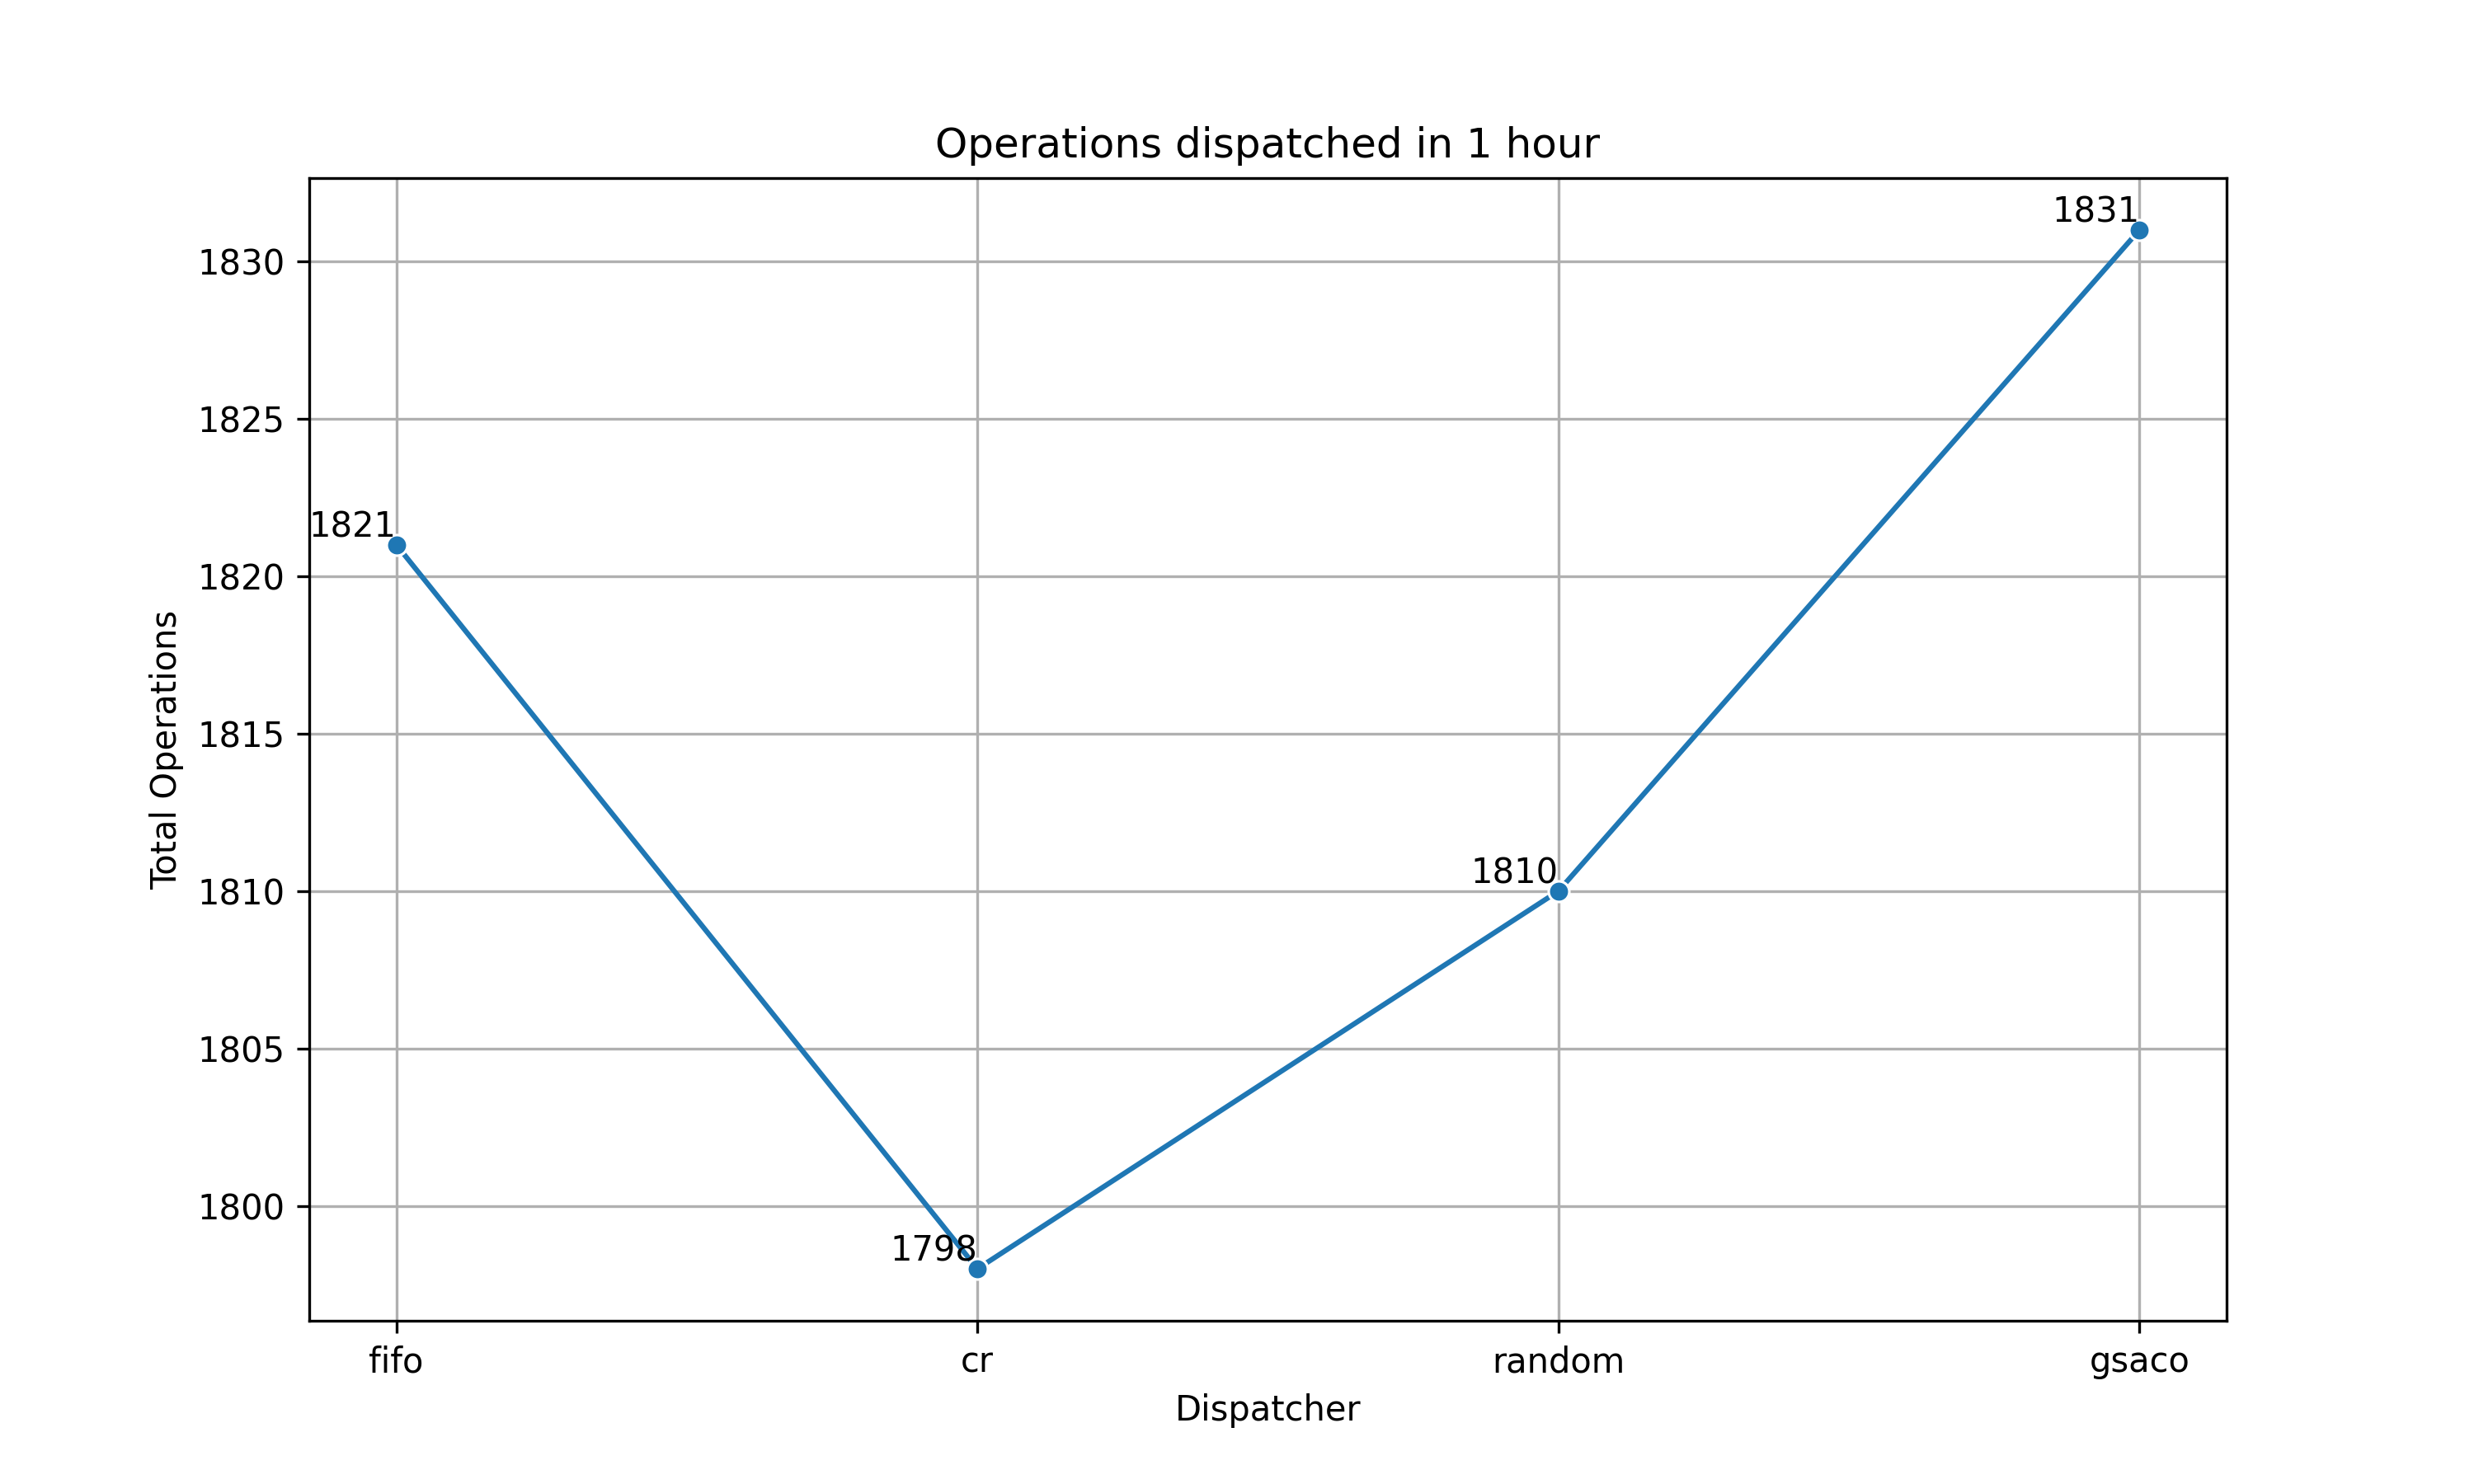
\includegraphics[width=\textwidth]{HVLM/total_operations_3600s.png}
		% \caption{}
		% \label{fig:o1}
	\end{subfigure}\hfill
	\begin{subfigure}{0.32\textwidth}
		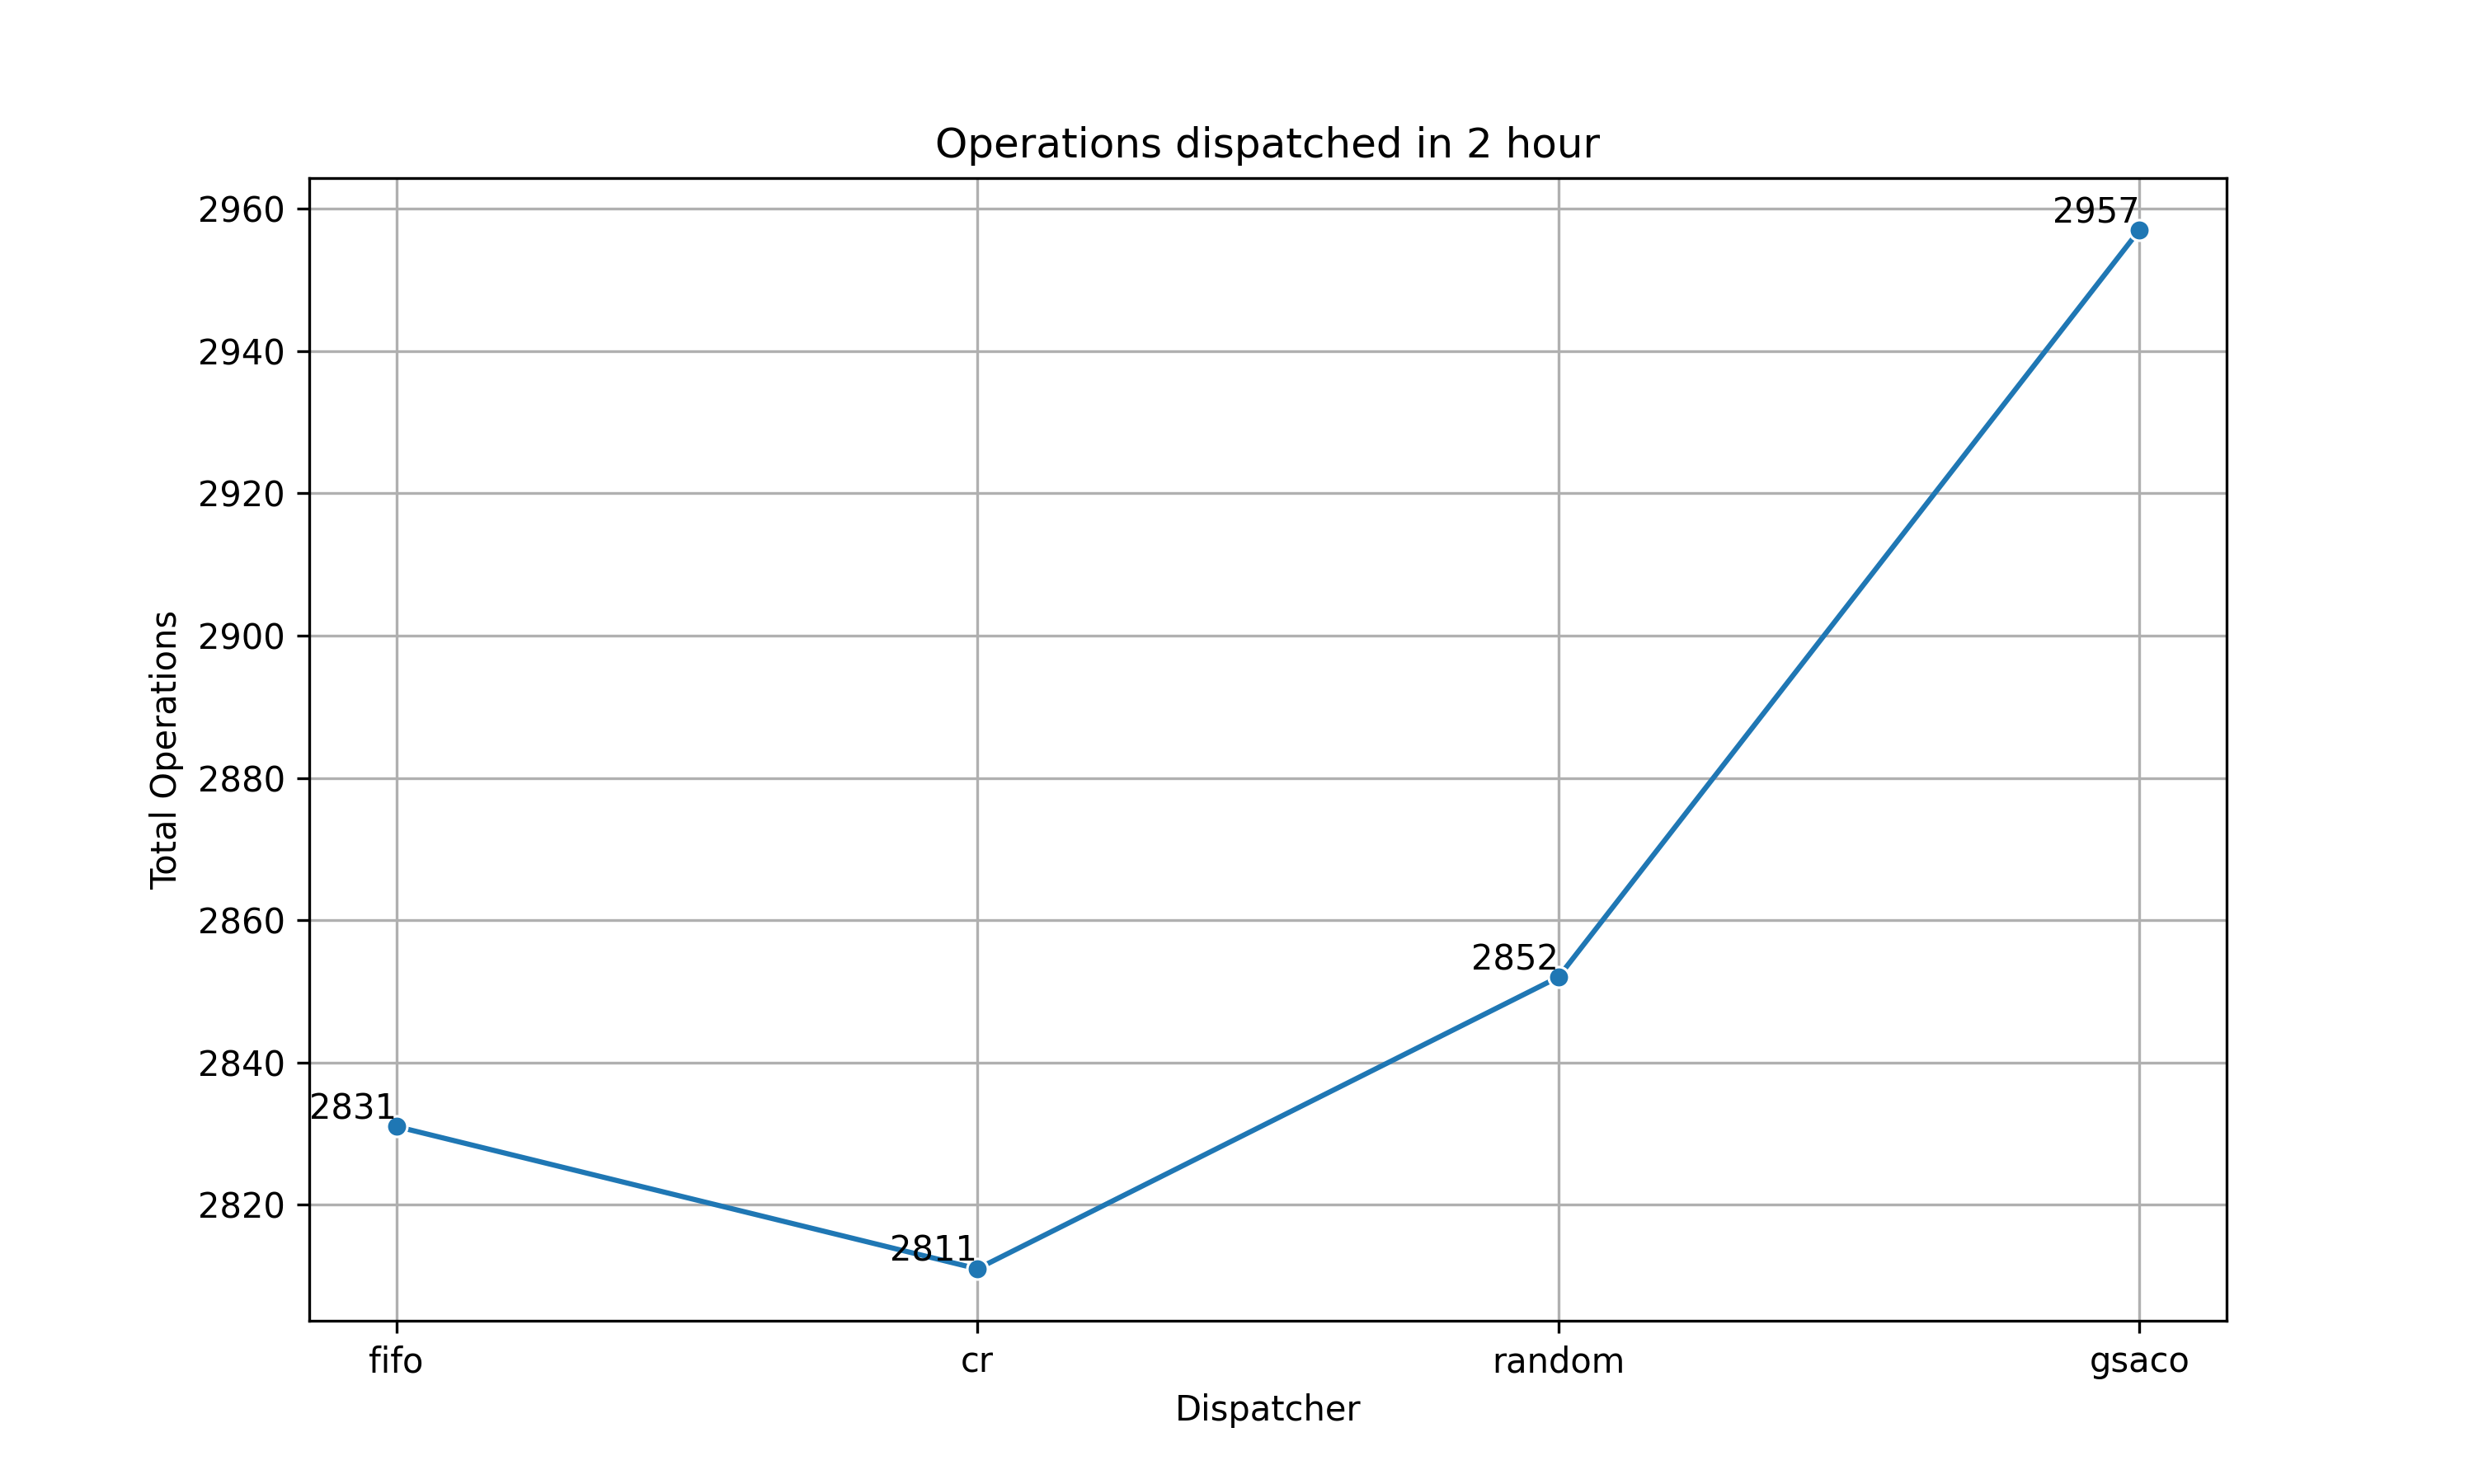
\includegraphics[width=\textwidth]{HVLM/total_operations_7200s.png}
		% \caption{}
		% \label{fig:o2}
	\end{subfigure}\hfill
	\begin{subfigure}{0.32\textwidth}
		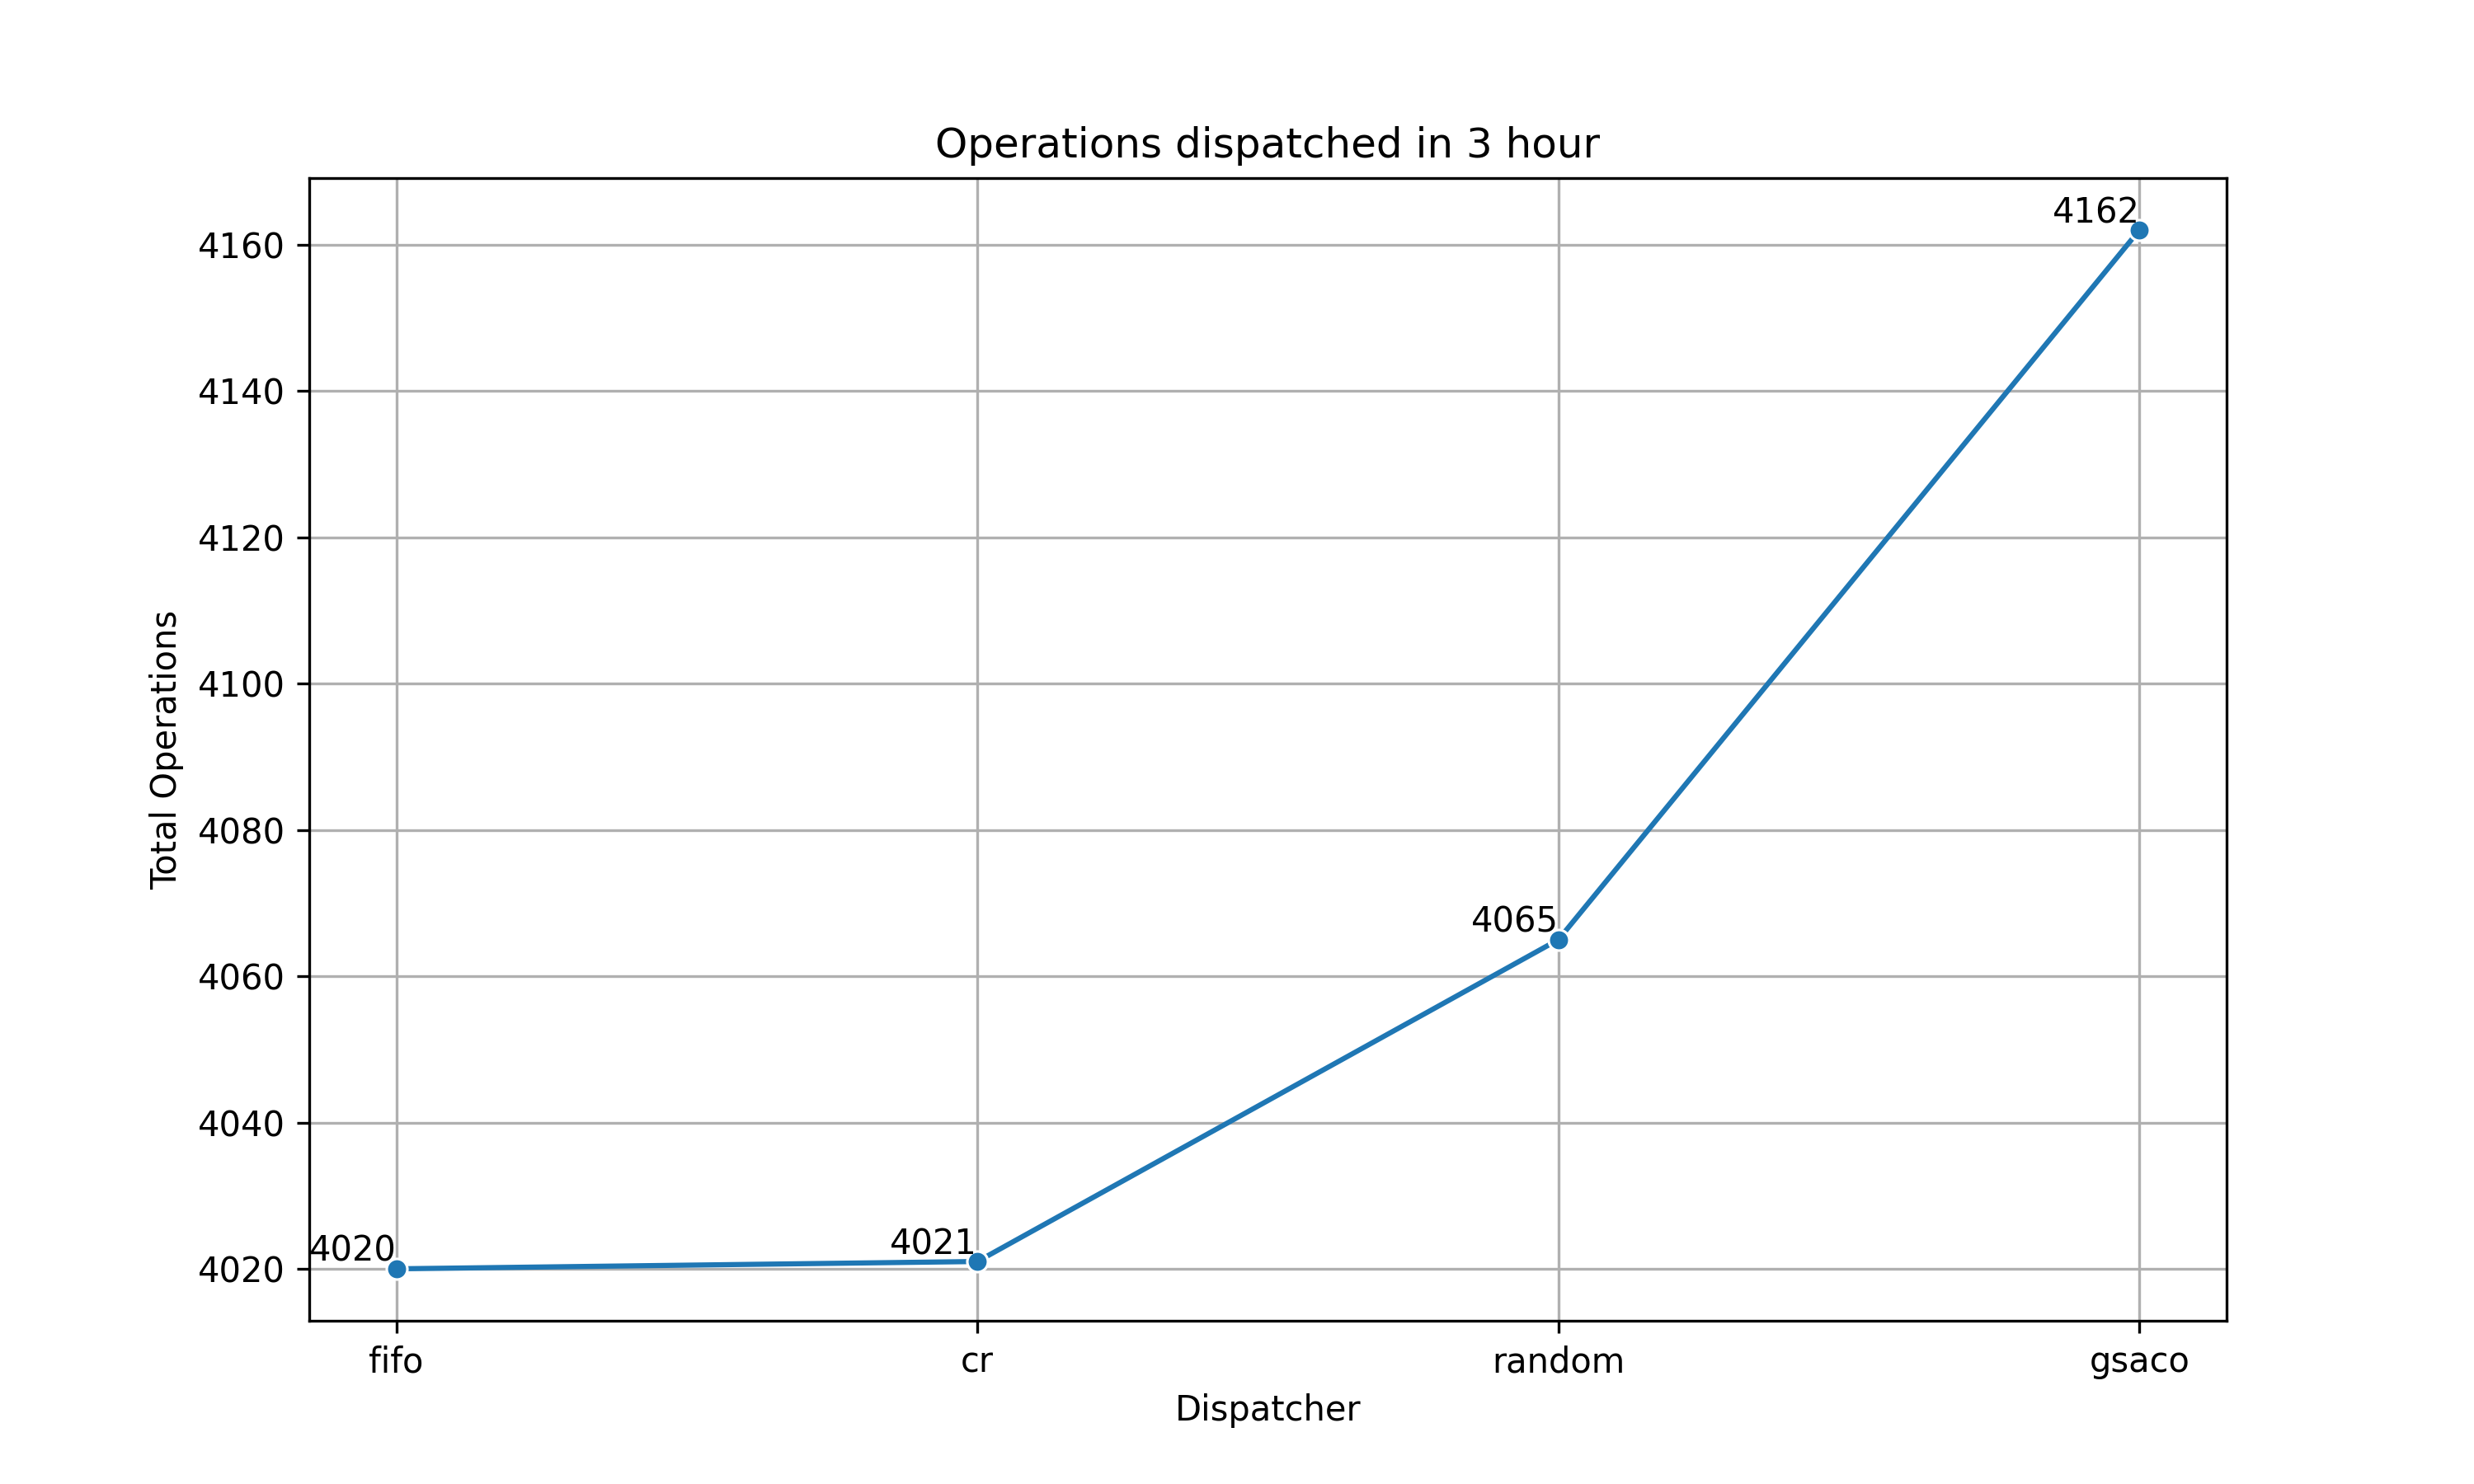
\includegraphics[width=\textwidth]{HVLM/total_operations_10800s.png}
		% \caption{}
		% \label{fig:o3}
	\end{subfigure}
	\begin{subfigure}{0.32\textwidth}
		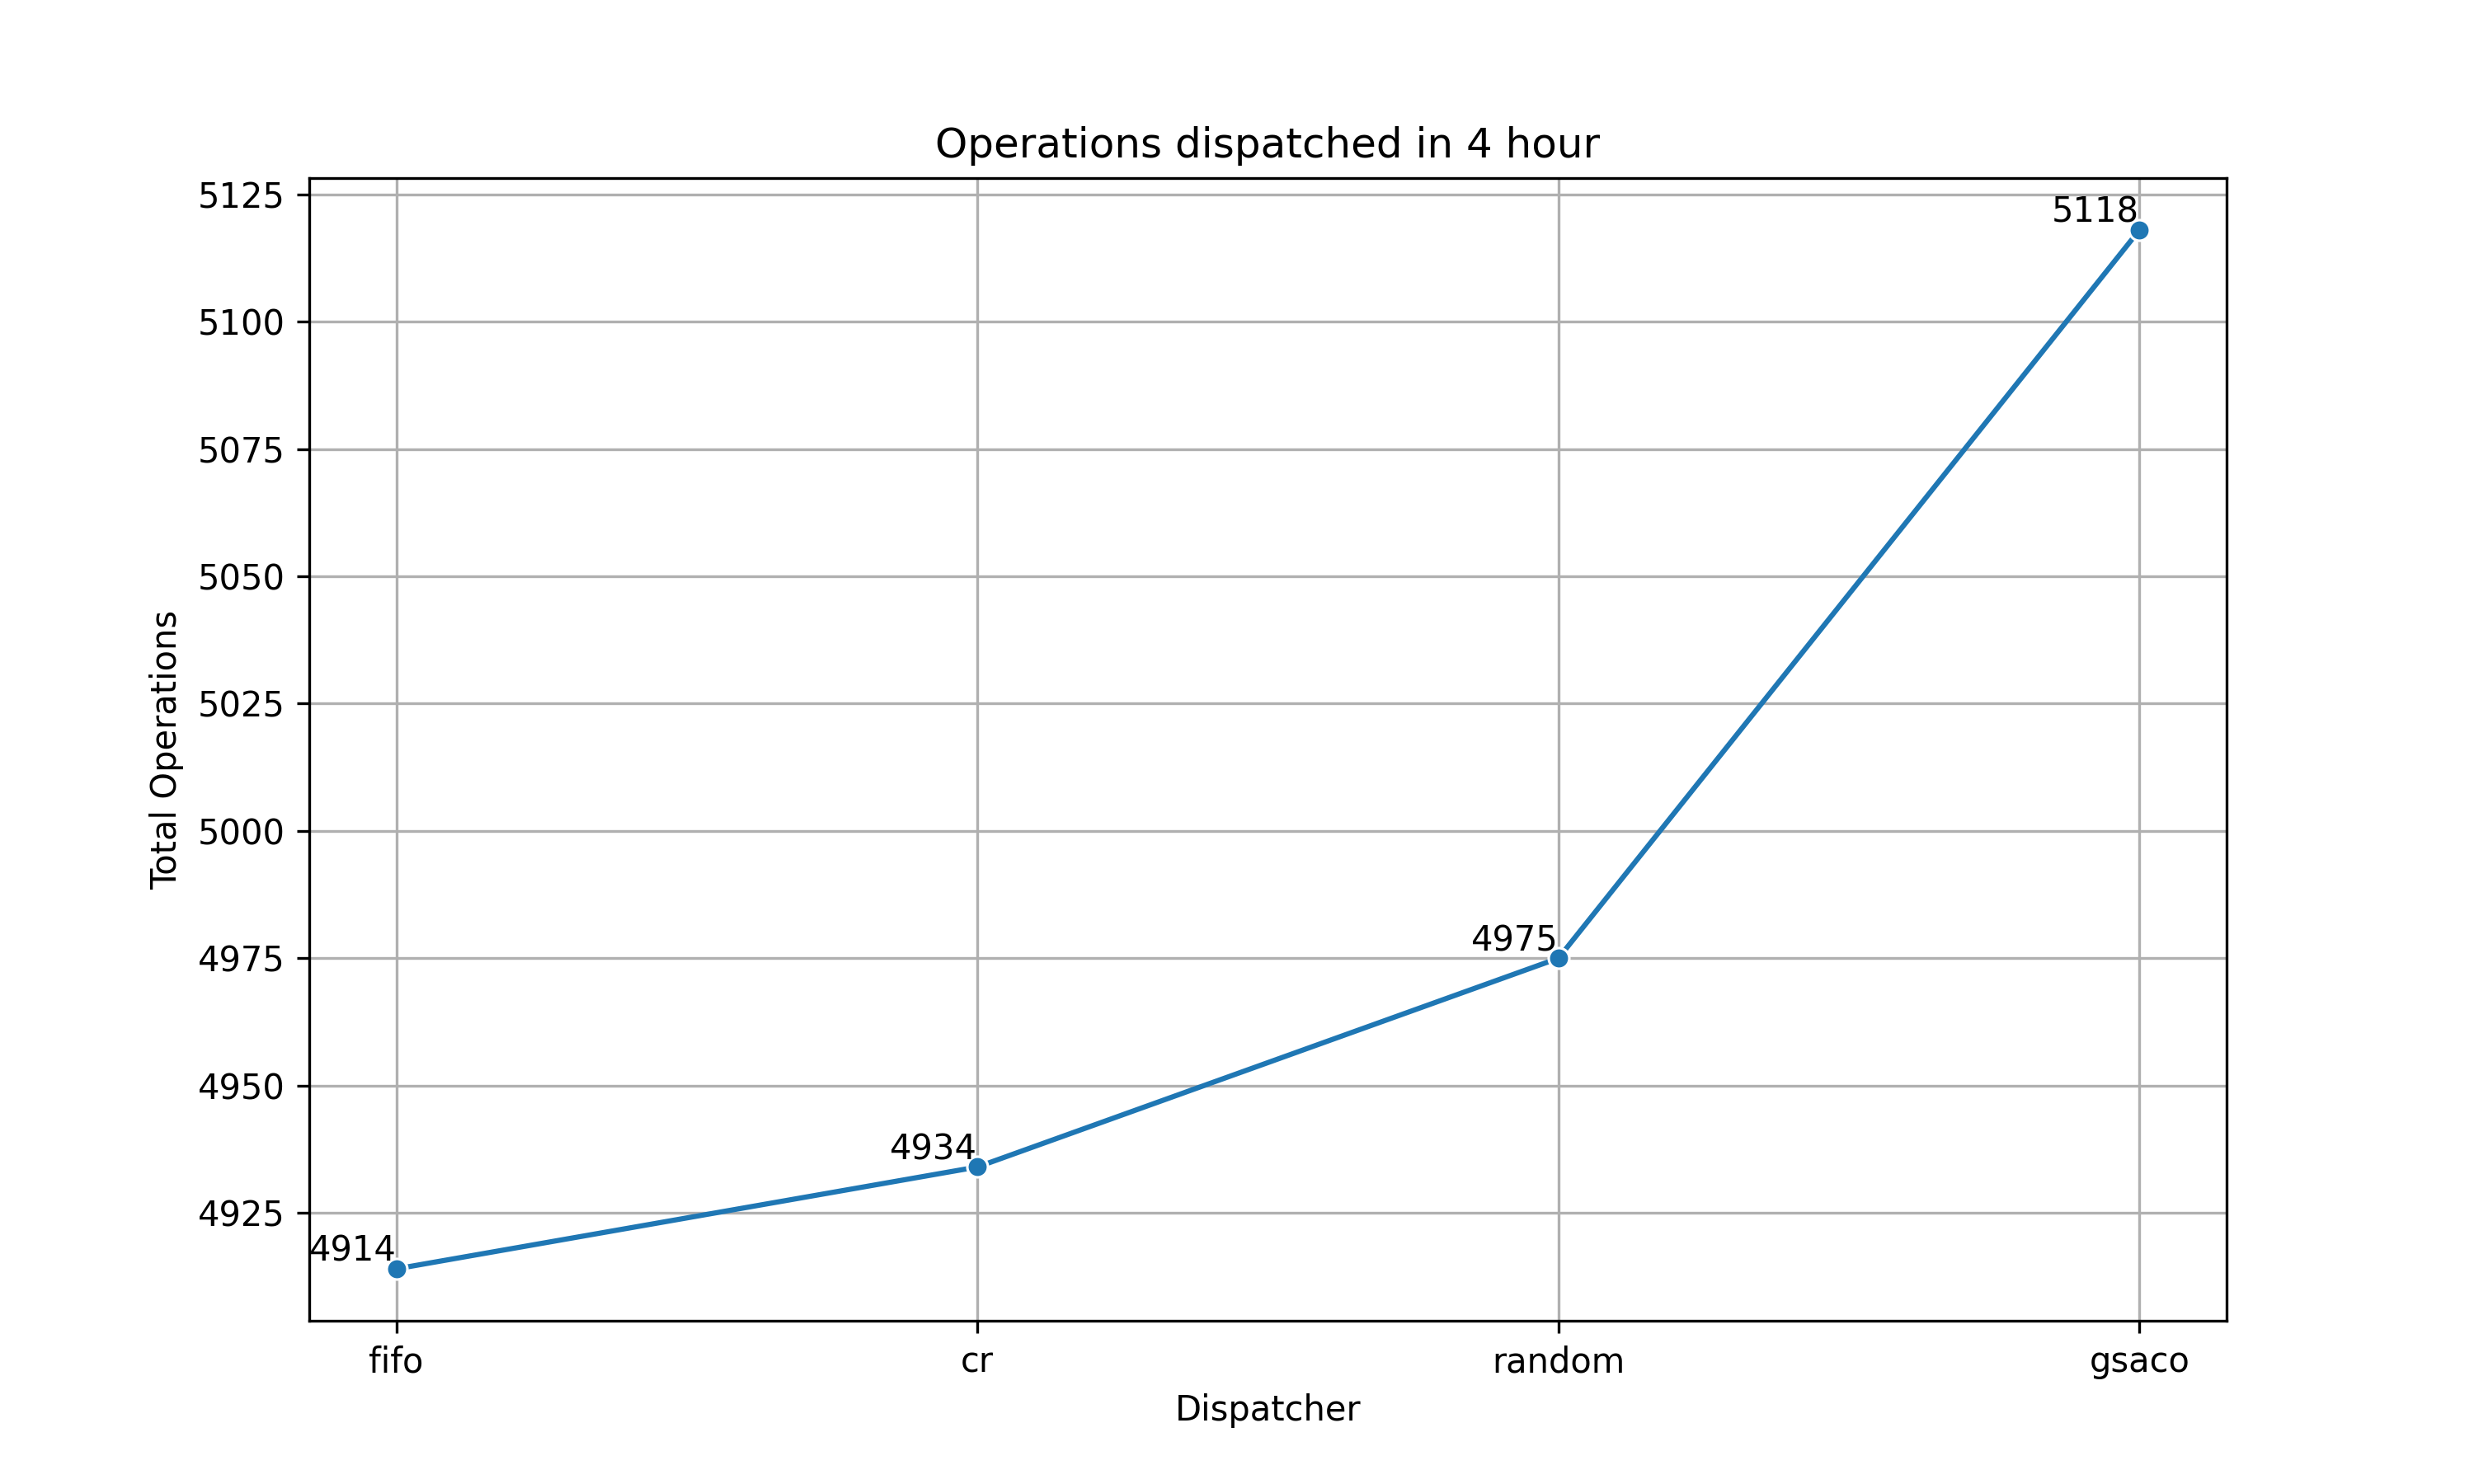
\includegraphics[width=\textwidth]{HVLM/total_operations_14400s.png}
		% \caption{}
		% \label{fig:o4}
	\end{subfigure}\hfill
	\begin{subfigure}{0.32\textwidth}
		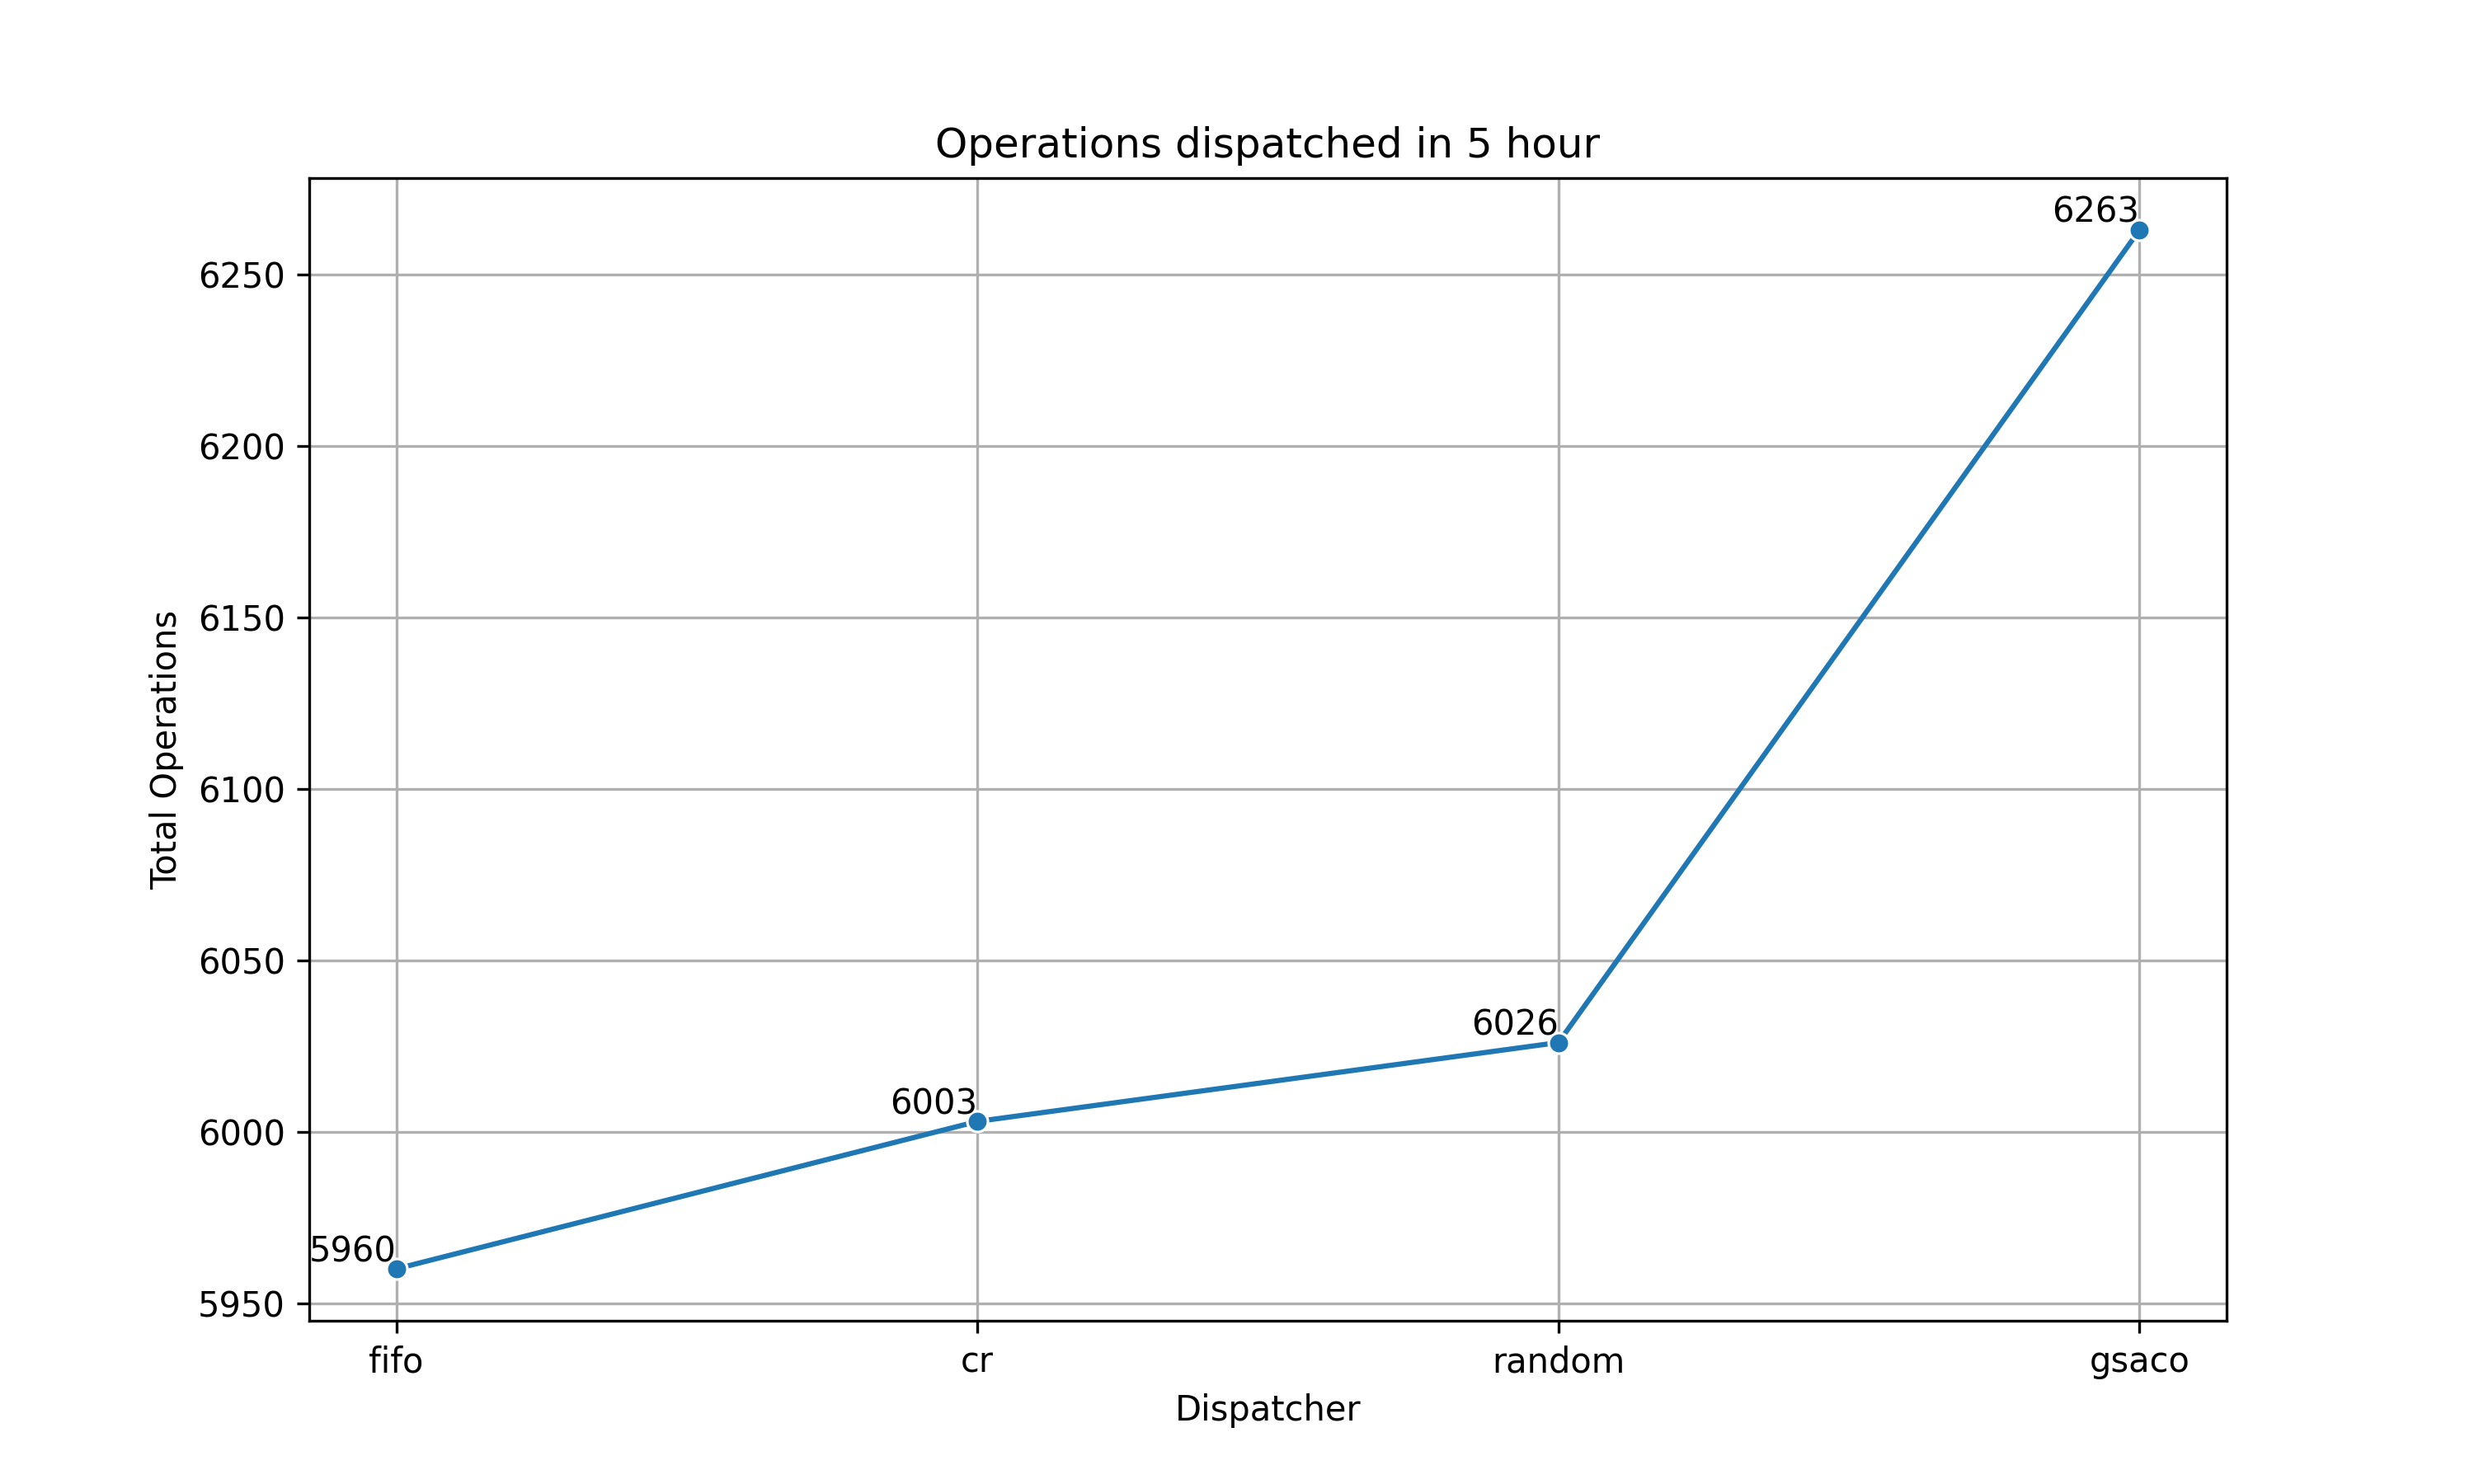
\includegraphics[width=\textwidth]{HVLM/total_operations_18000s.png}
		% \caption{}
		% \label{fig:o5}
	\end{subfigure}\hfill
	\begin{subfigure}{0.32\textwidth}
		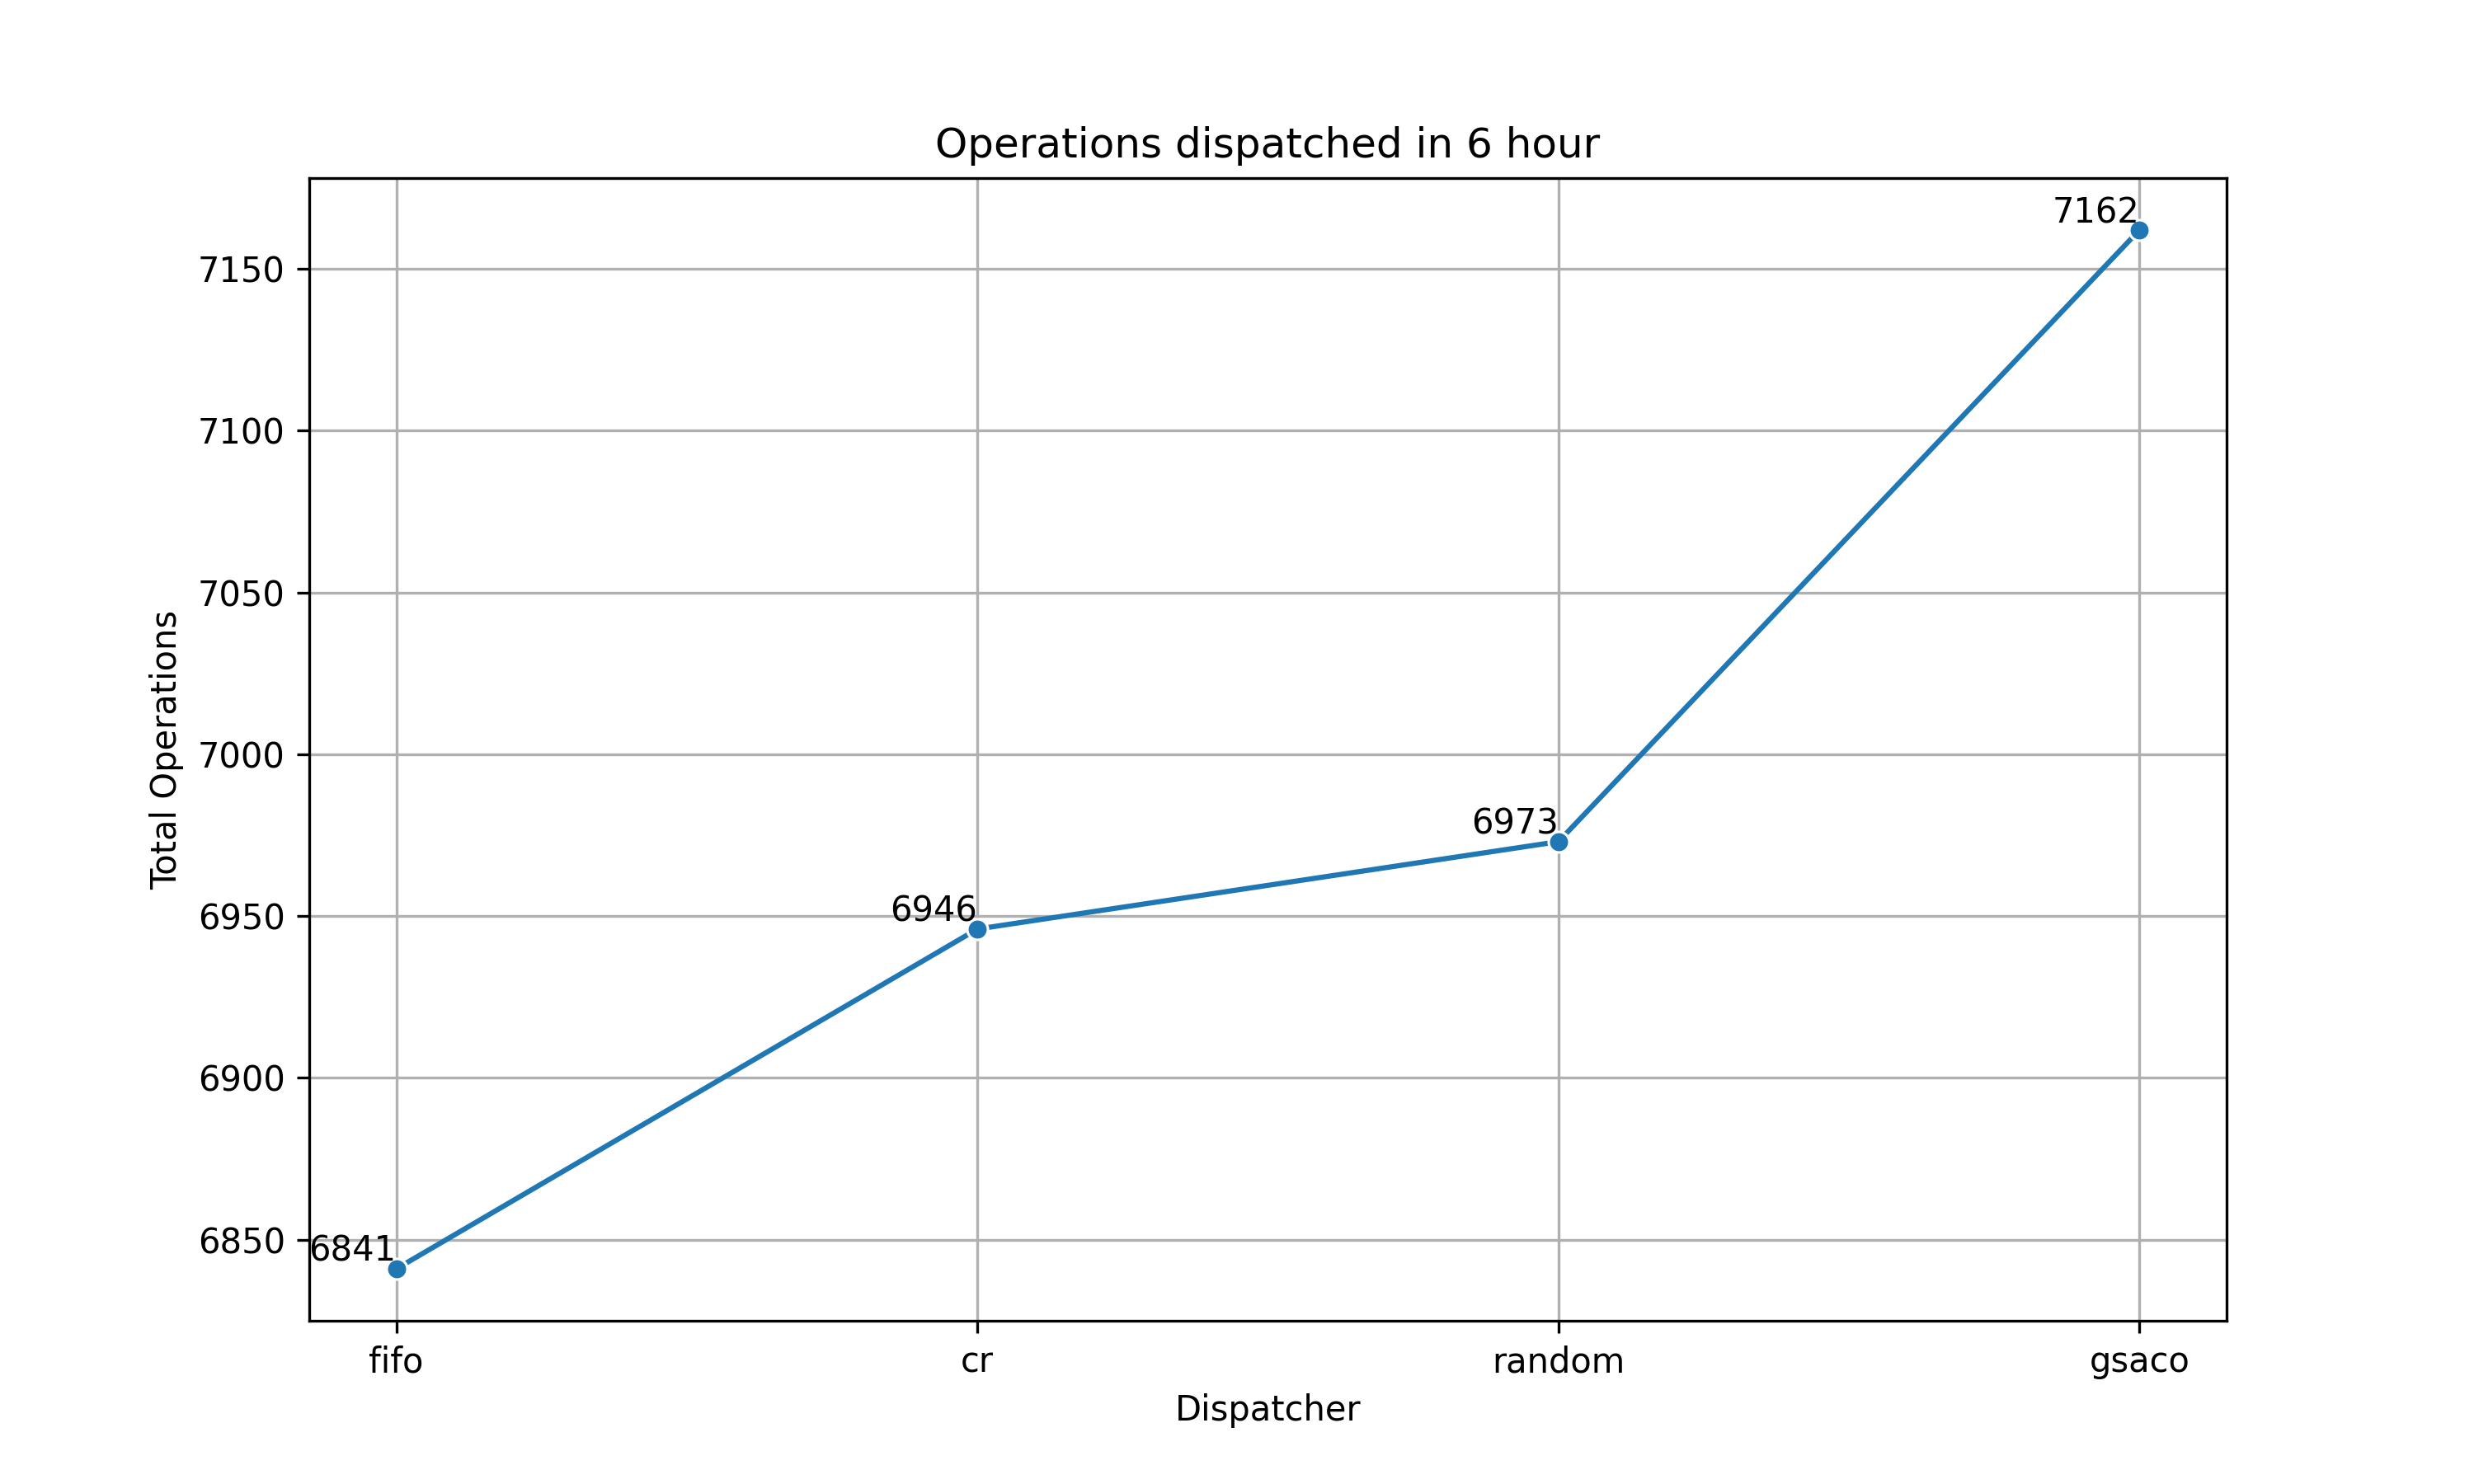
\includegraphics[width=\textwidth]{HVLM/total_operations_21600s.png}
		% \caption{}
		% \label{fig:o6}
	\end{subfigure}
	\caption{Completed operations for HV/LM}
	\label{fig:totalopsHVLM}
\end{figure}

\begin{figure}[t]
	\centering
	\begin{subfigure}[b]{0.32\textwidth}
		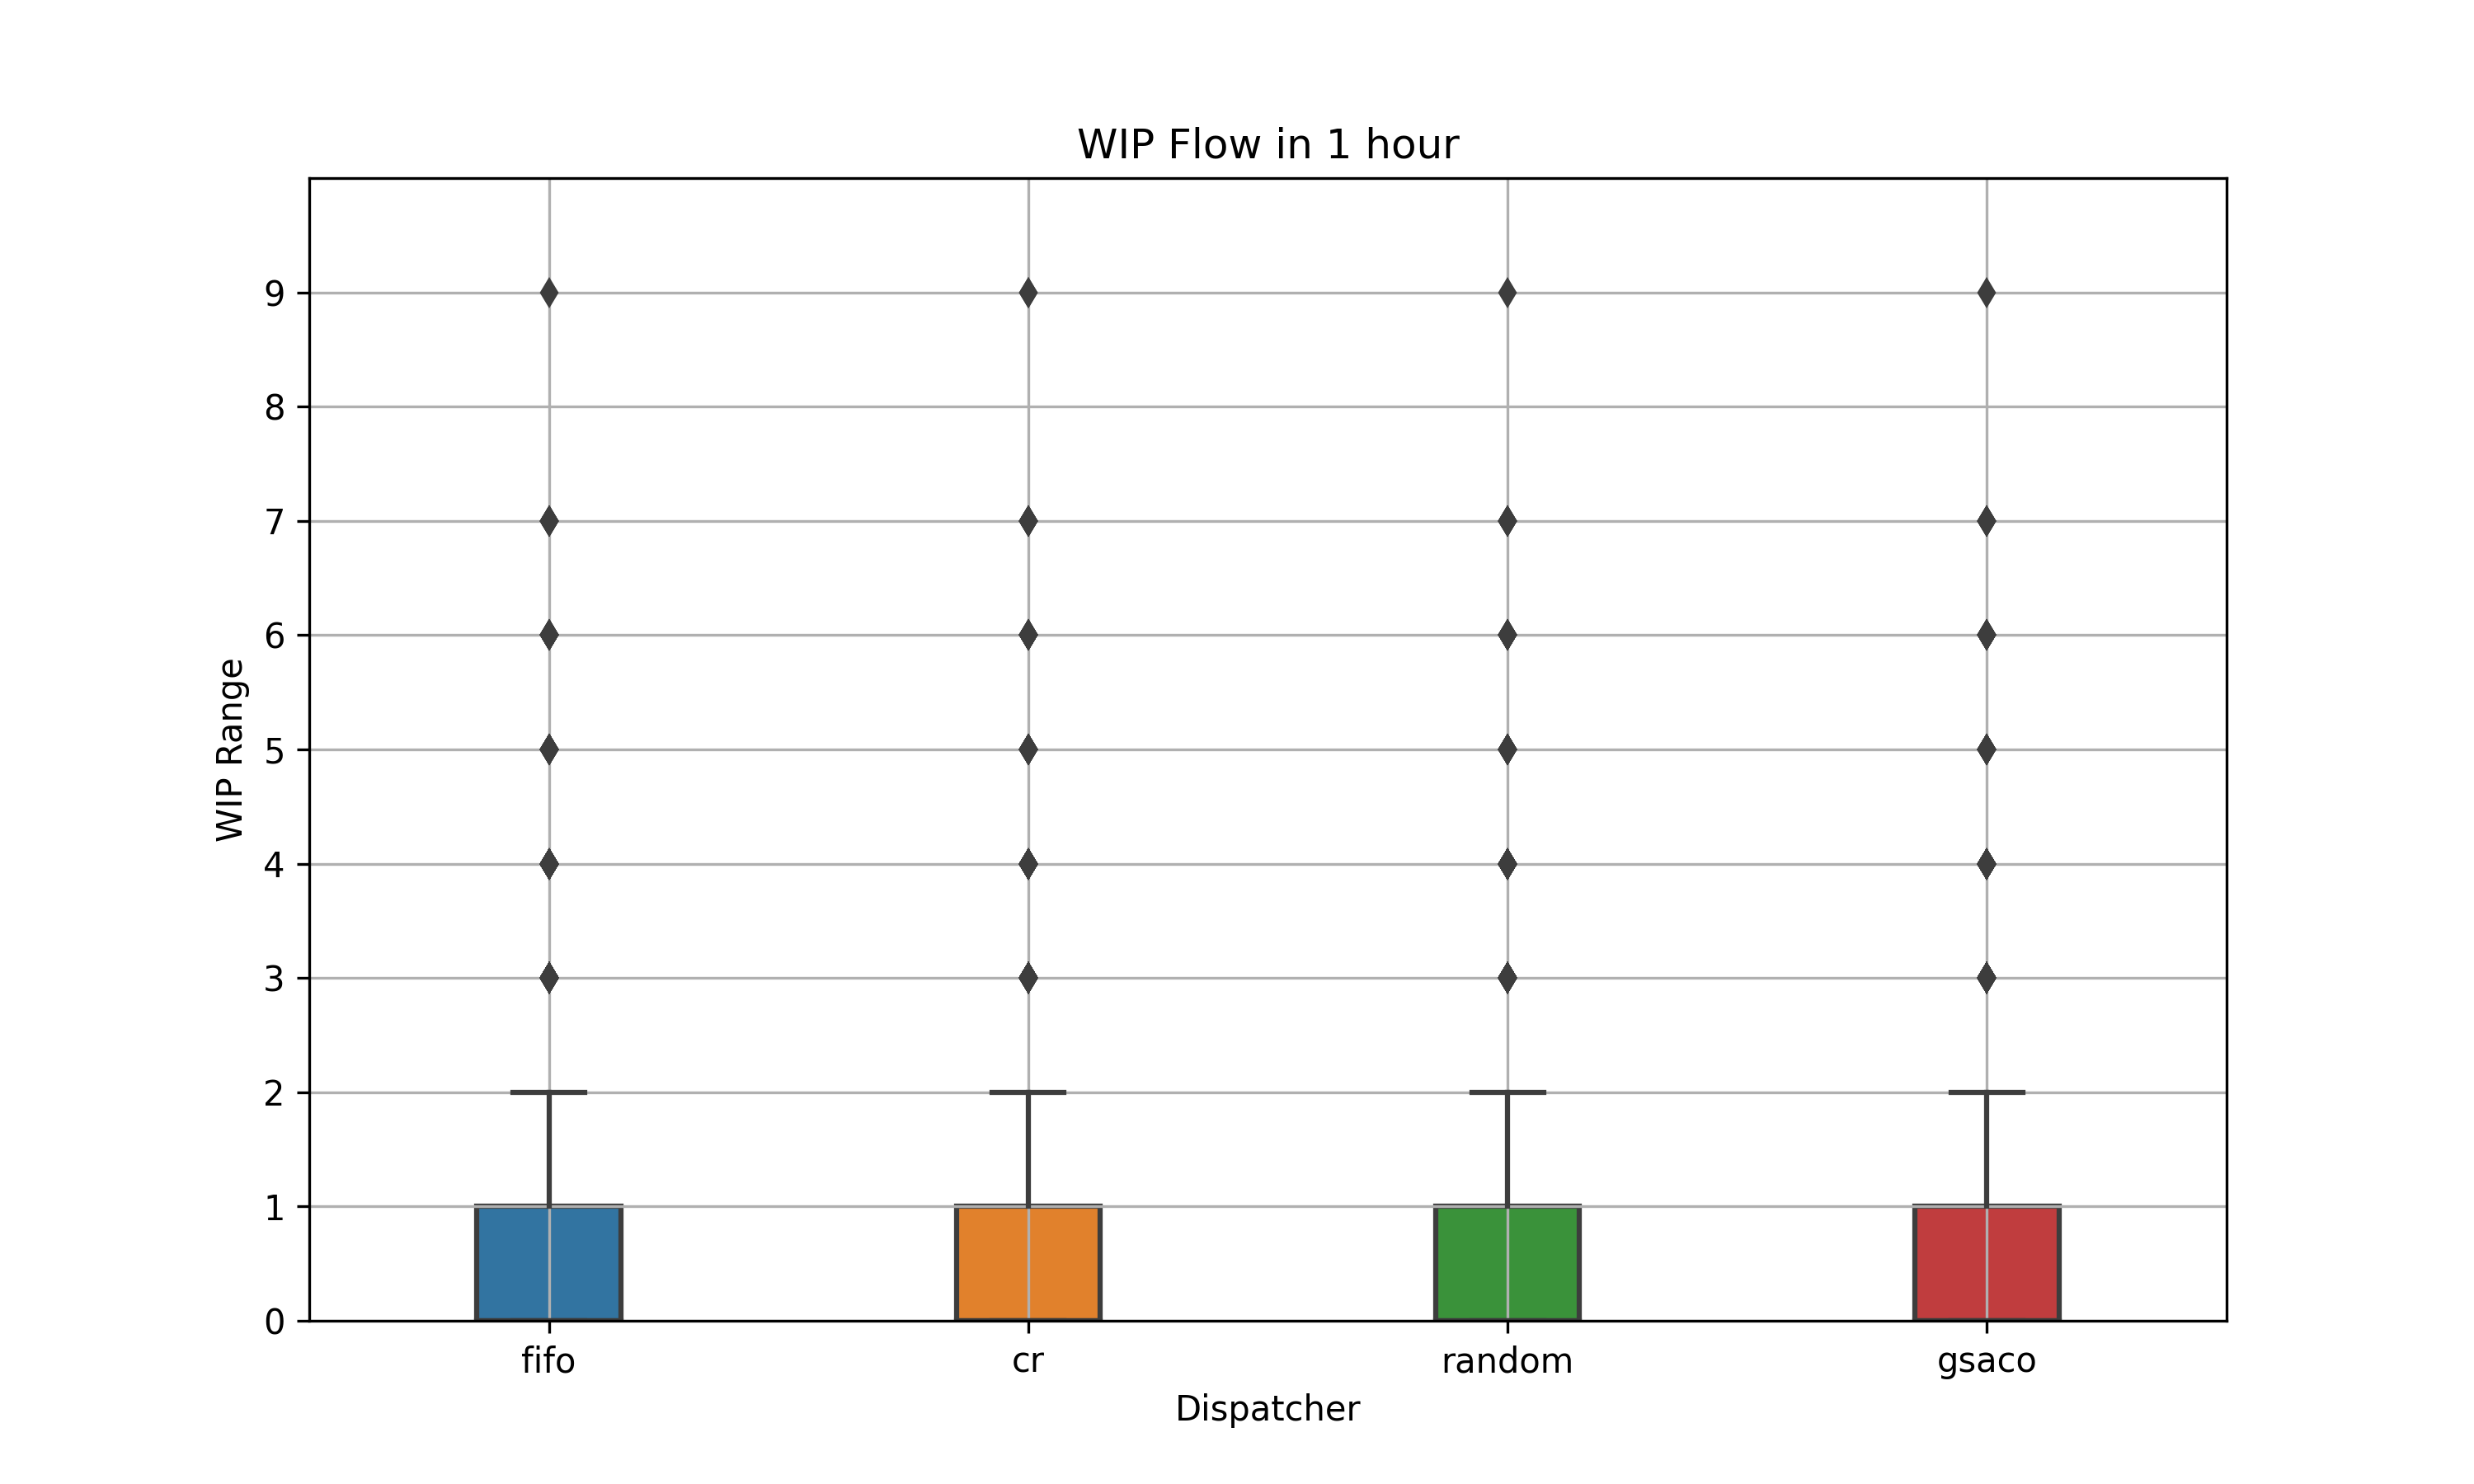
\includegraphics[width=\textwidth]{HVLM/period_3600s.png}
		% \caption{}
		% \label{fig:p1}
	\end{subfigure}
	\hfill
	\begin{subfigure}[b]{0.32\textwidth}
		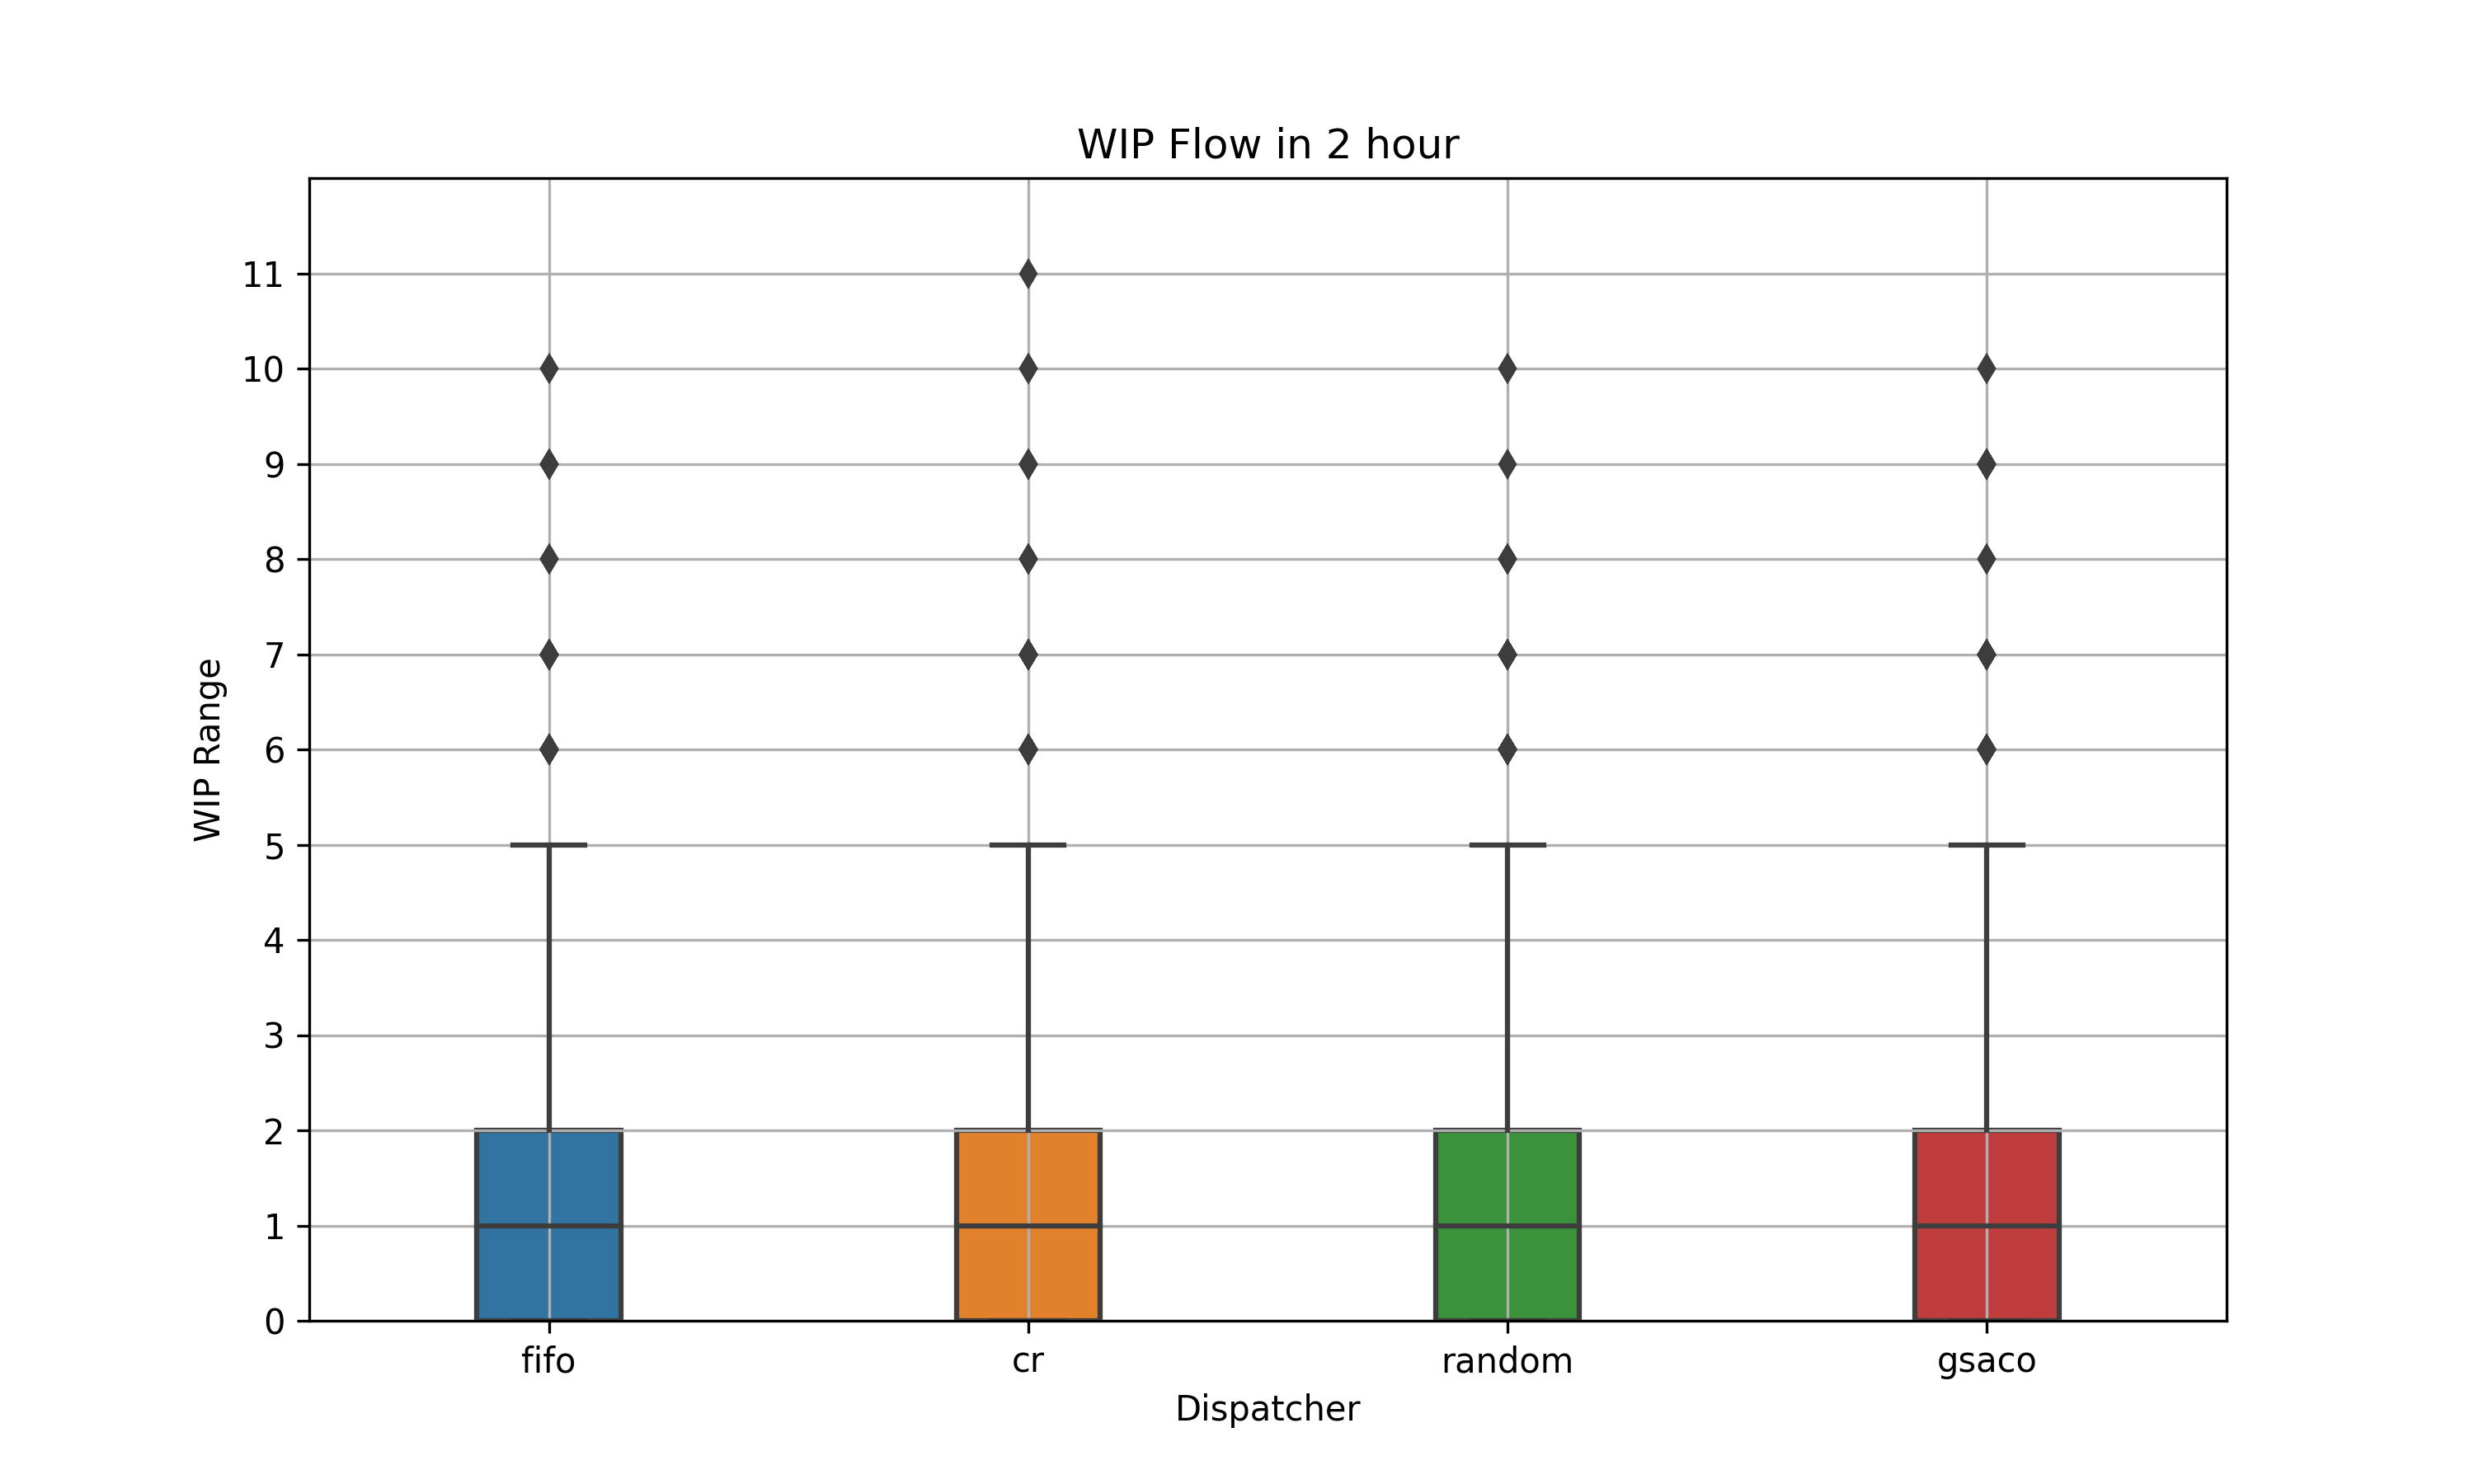
\includegraphics[width=\textwidth]{HVLM/period_7200s.png}
		% \caption{}
		% \label{fig:p2}
	\end{subfigure}
	\hfill
	\begin{subfigure}[b]{0.32\textwidth}
		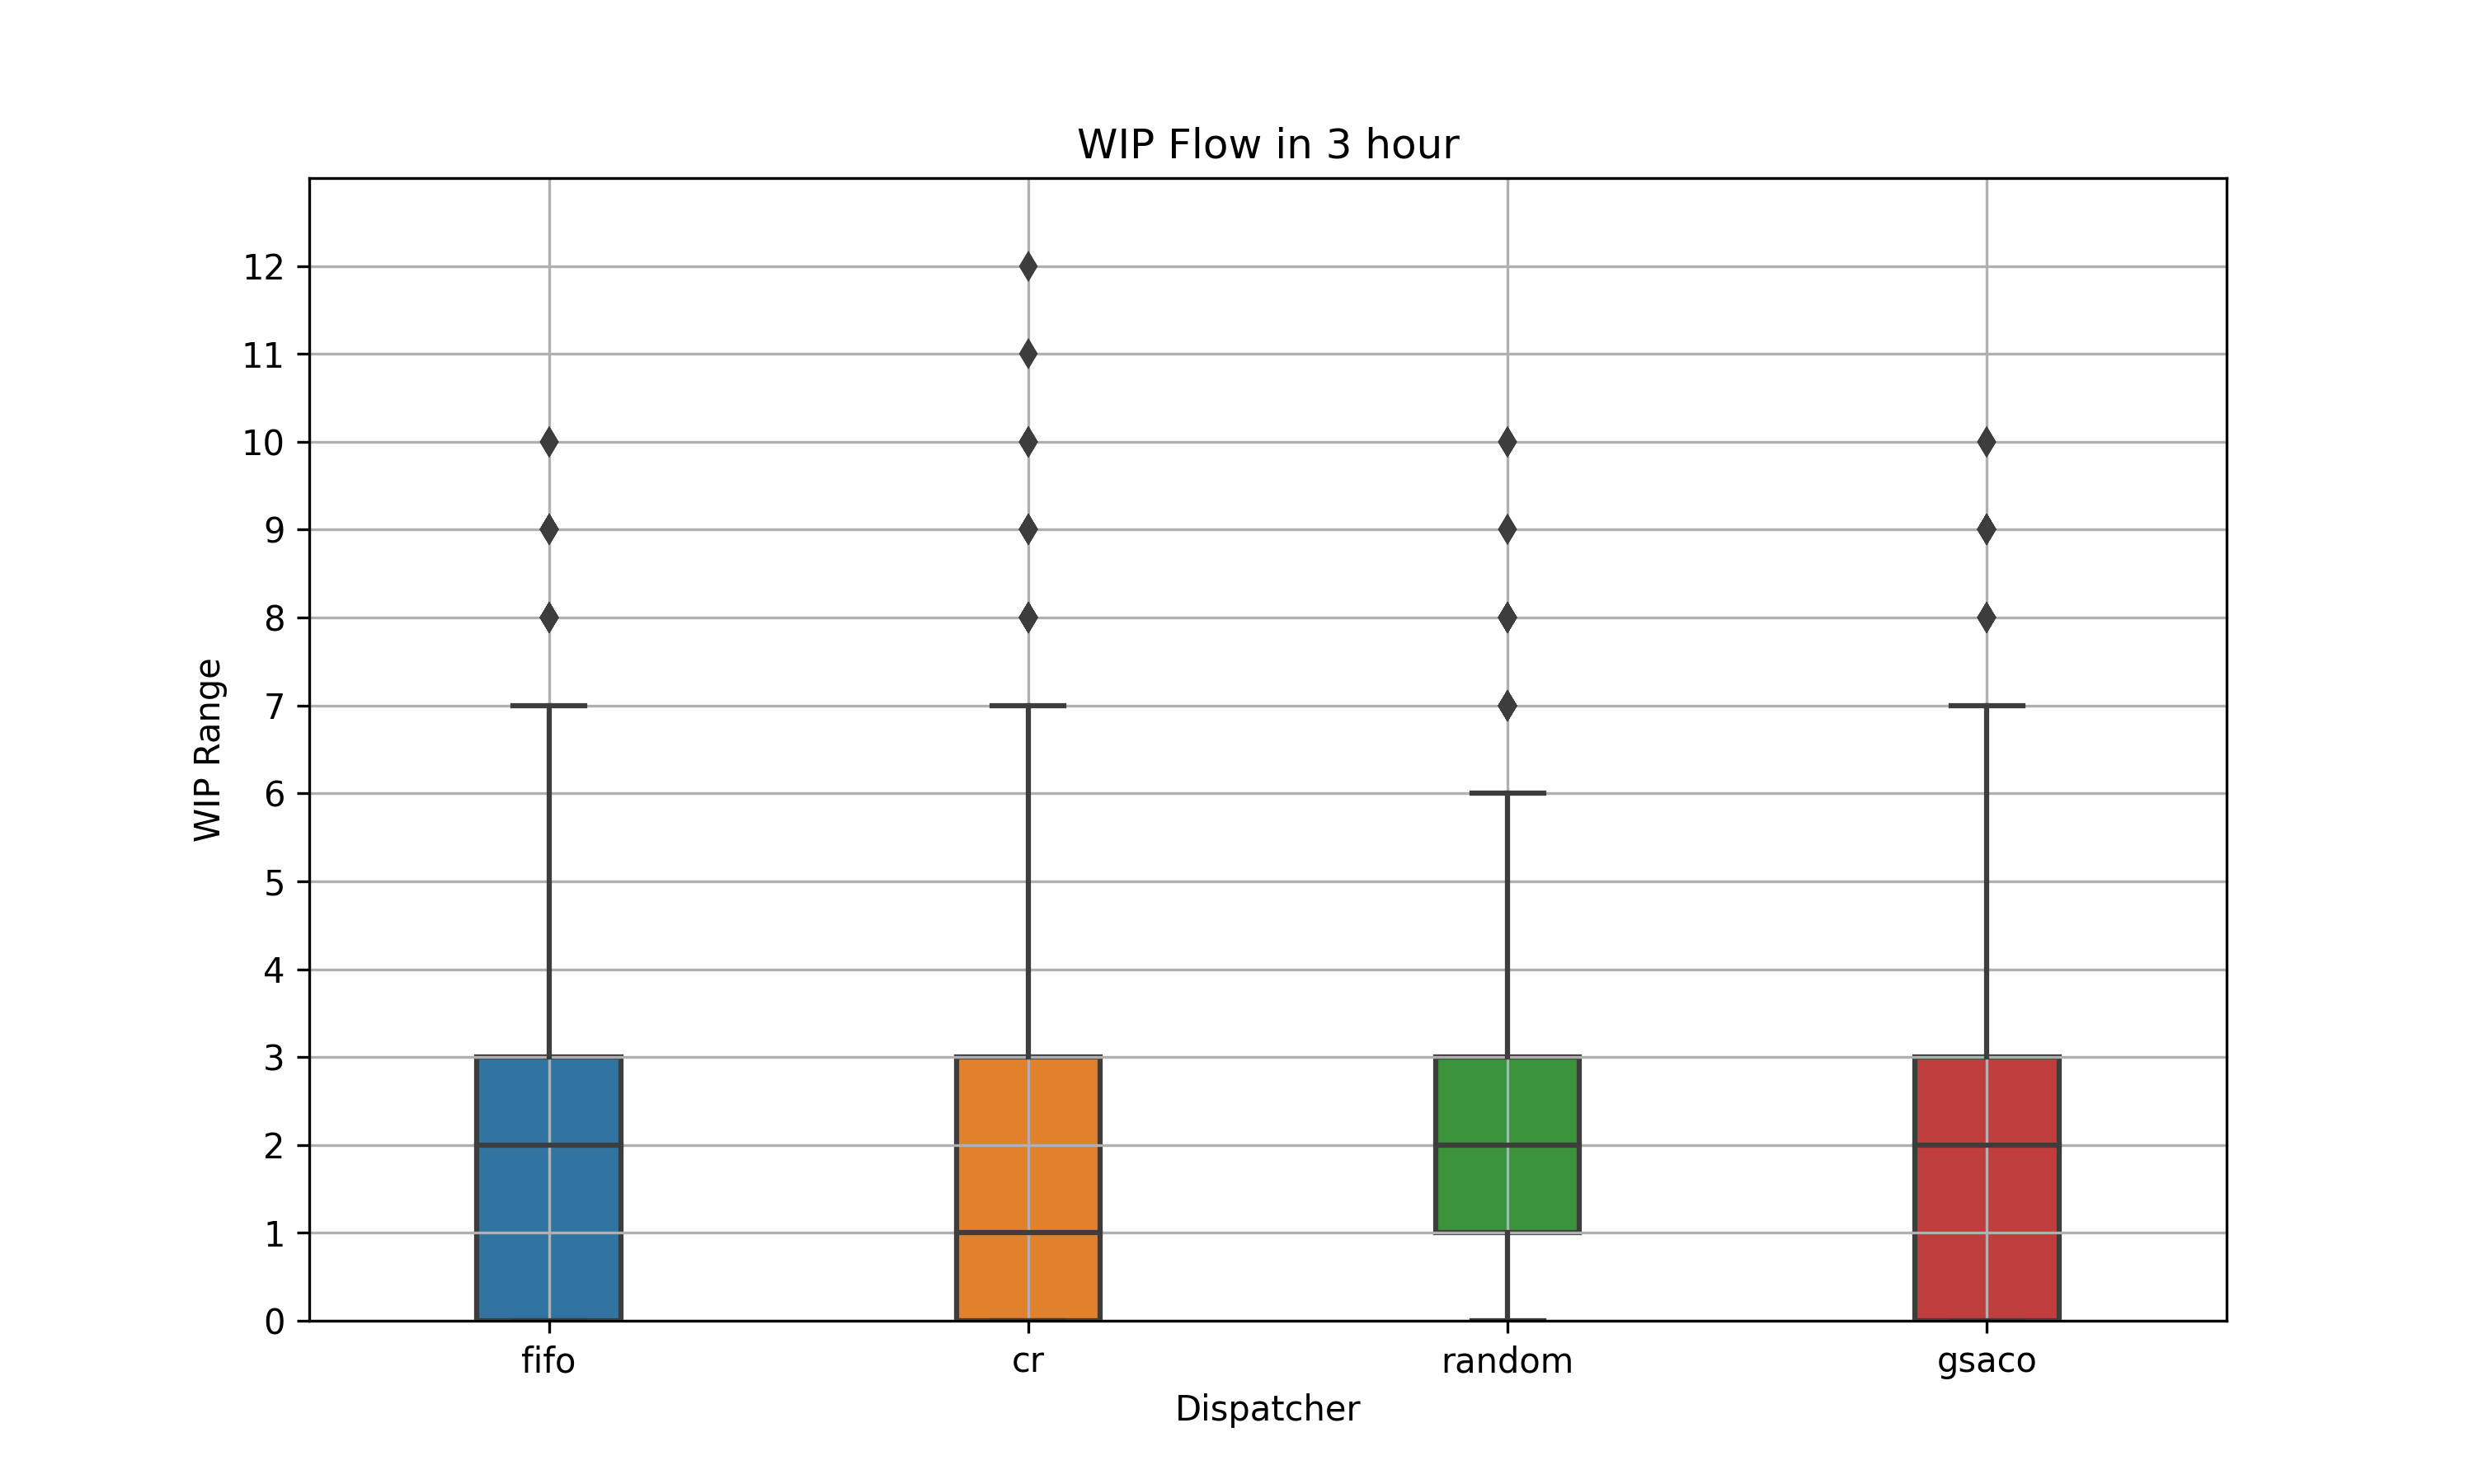
\includegraphics[width=\textwidth]{HVLM/period_10800s.png}
		% \caption{}
		% \label{fig:p3}
	\end{subfigure}
	
	\begin{subfigure}[b]{0.32\textwidth}
		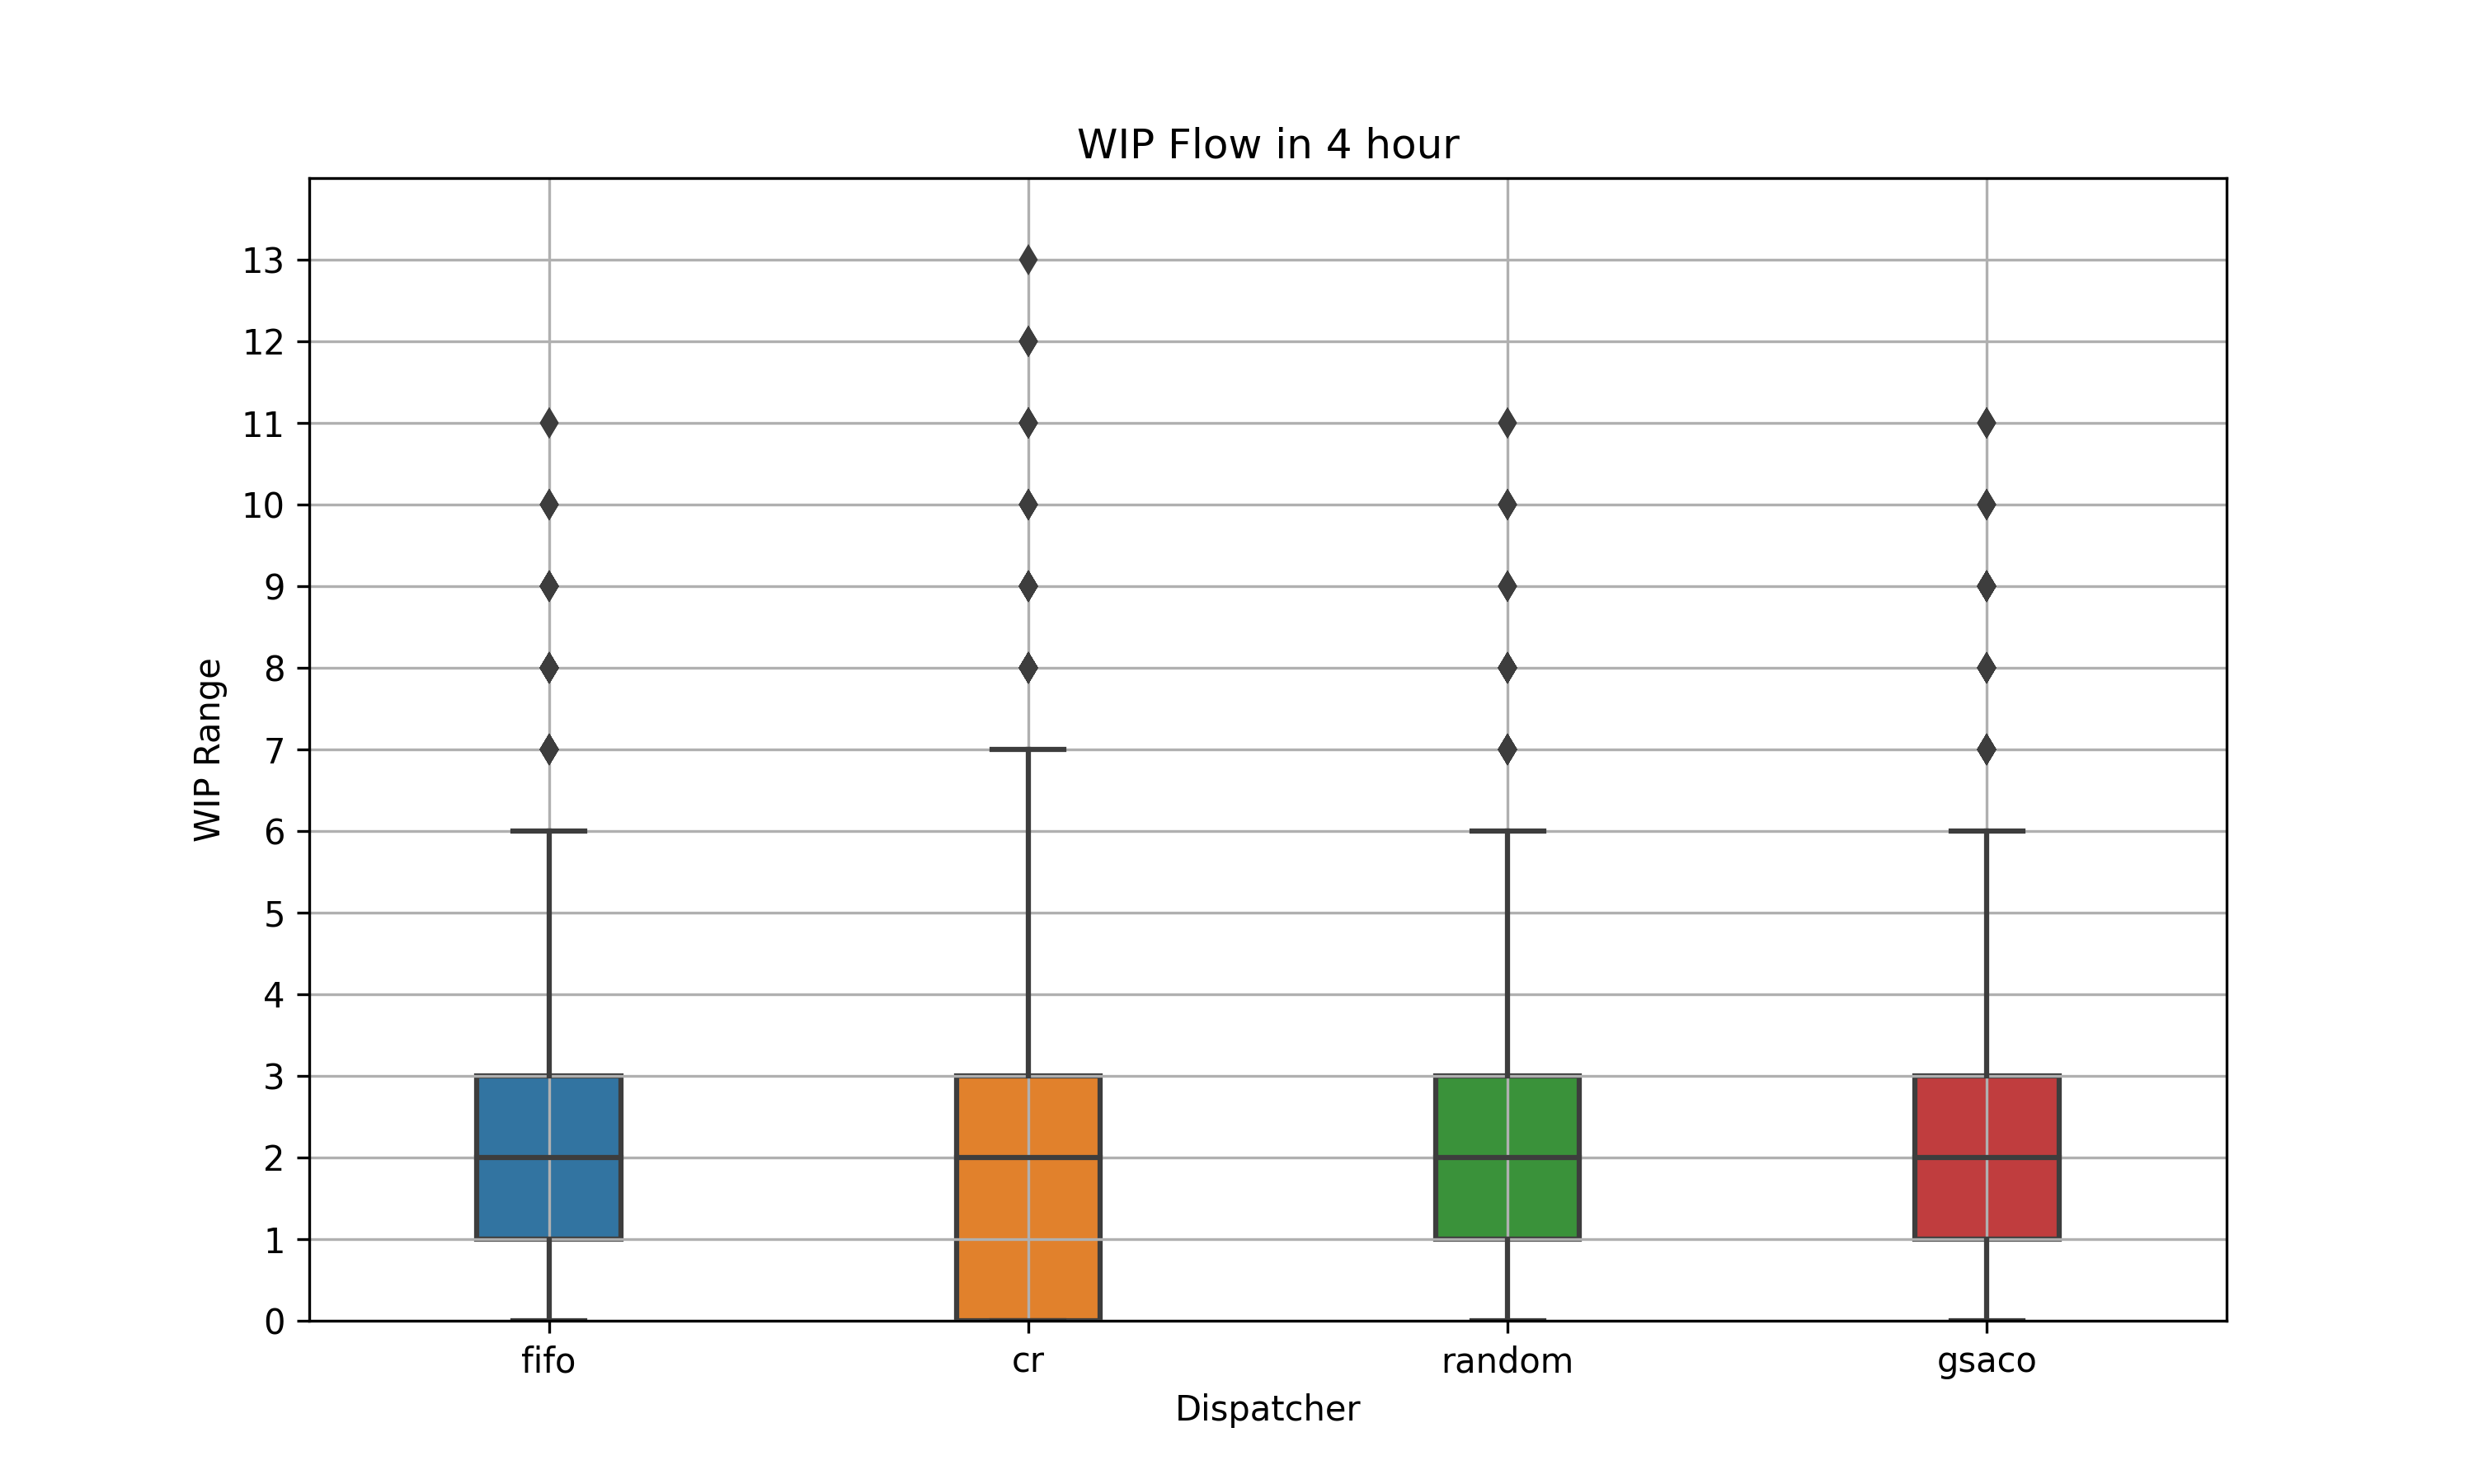
\includegraphics[width=\textwidth]{HVLM/period_14400s.png}
		% \caption{}
		% \label{fig:p4}
	\end{subfigure}
	\hfill
	\begin{subfigure}[b]{0.32\textwidth}
		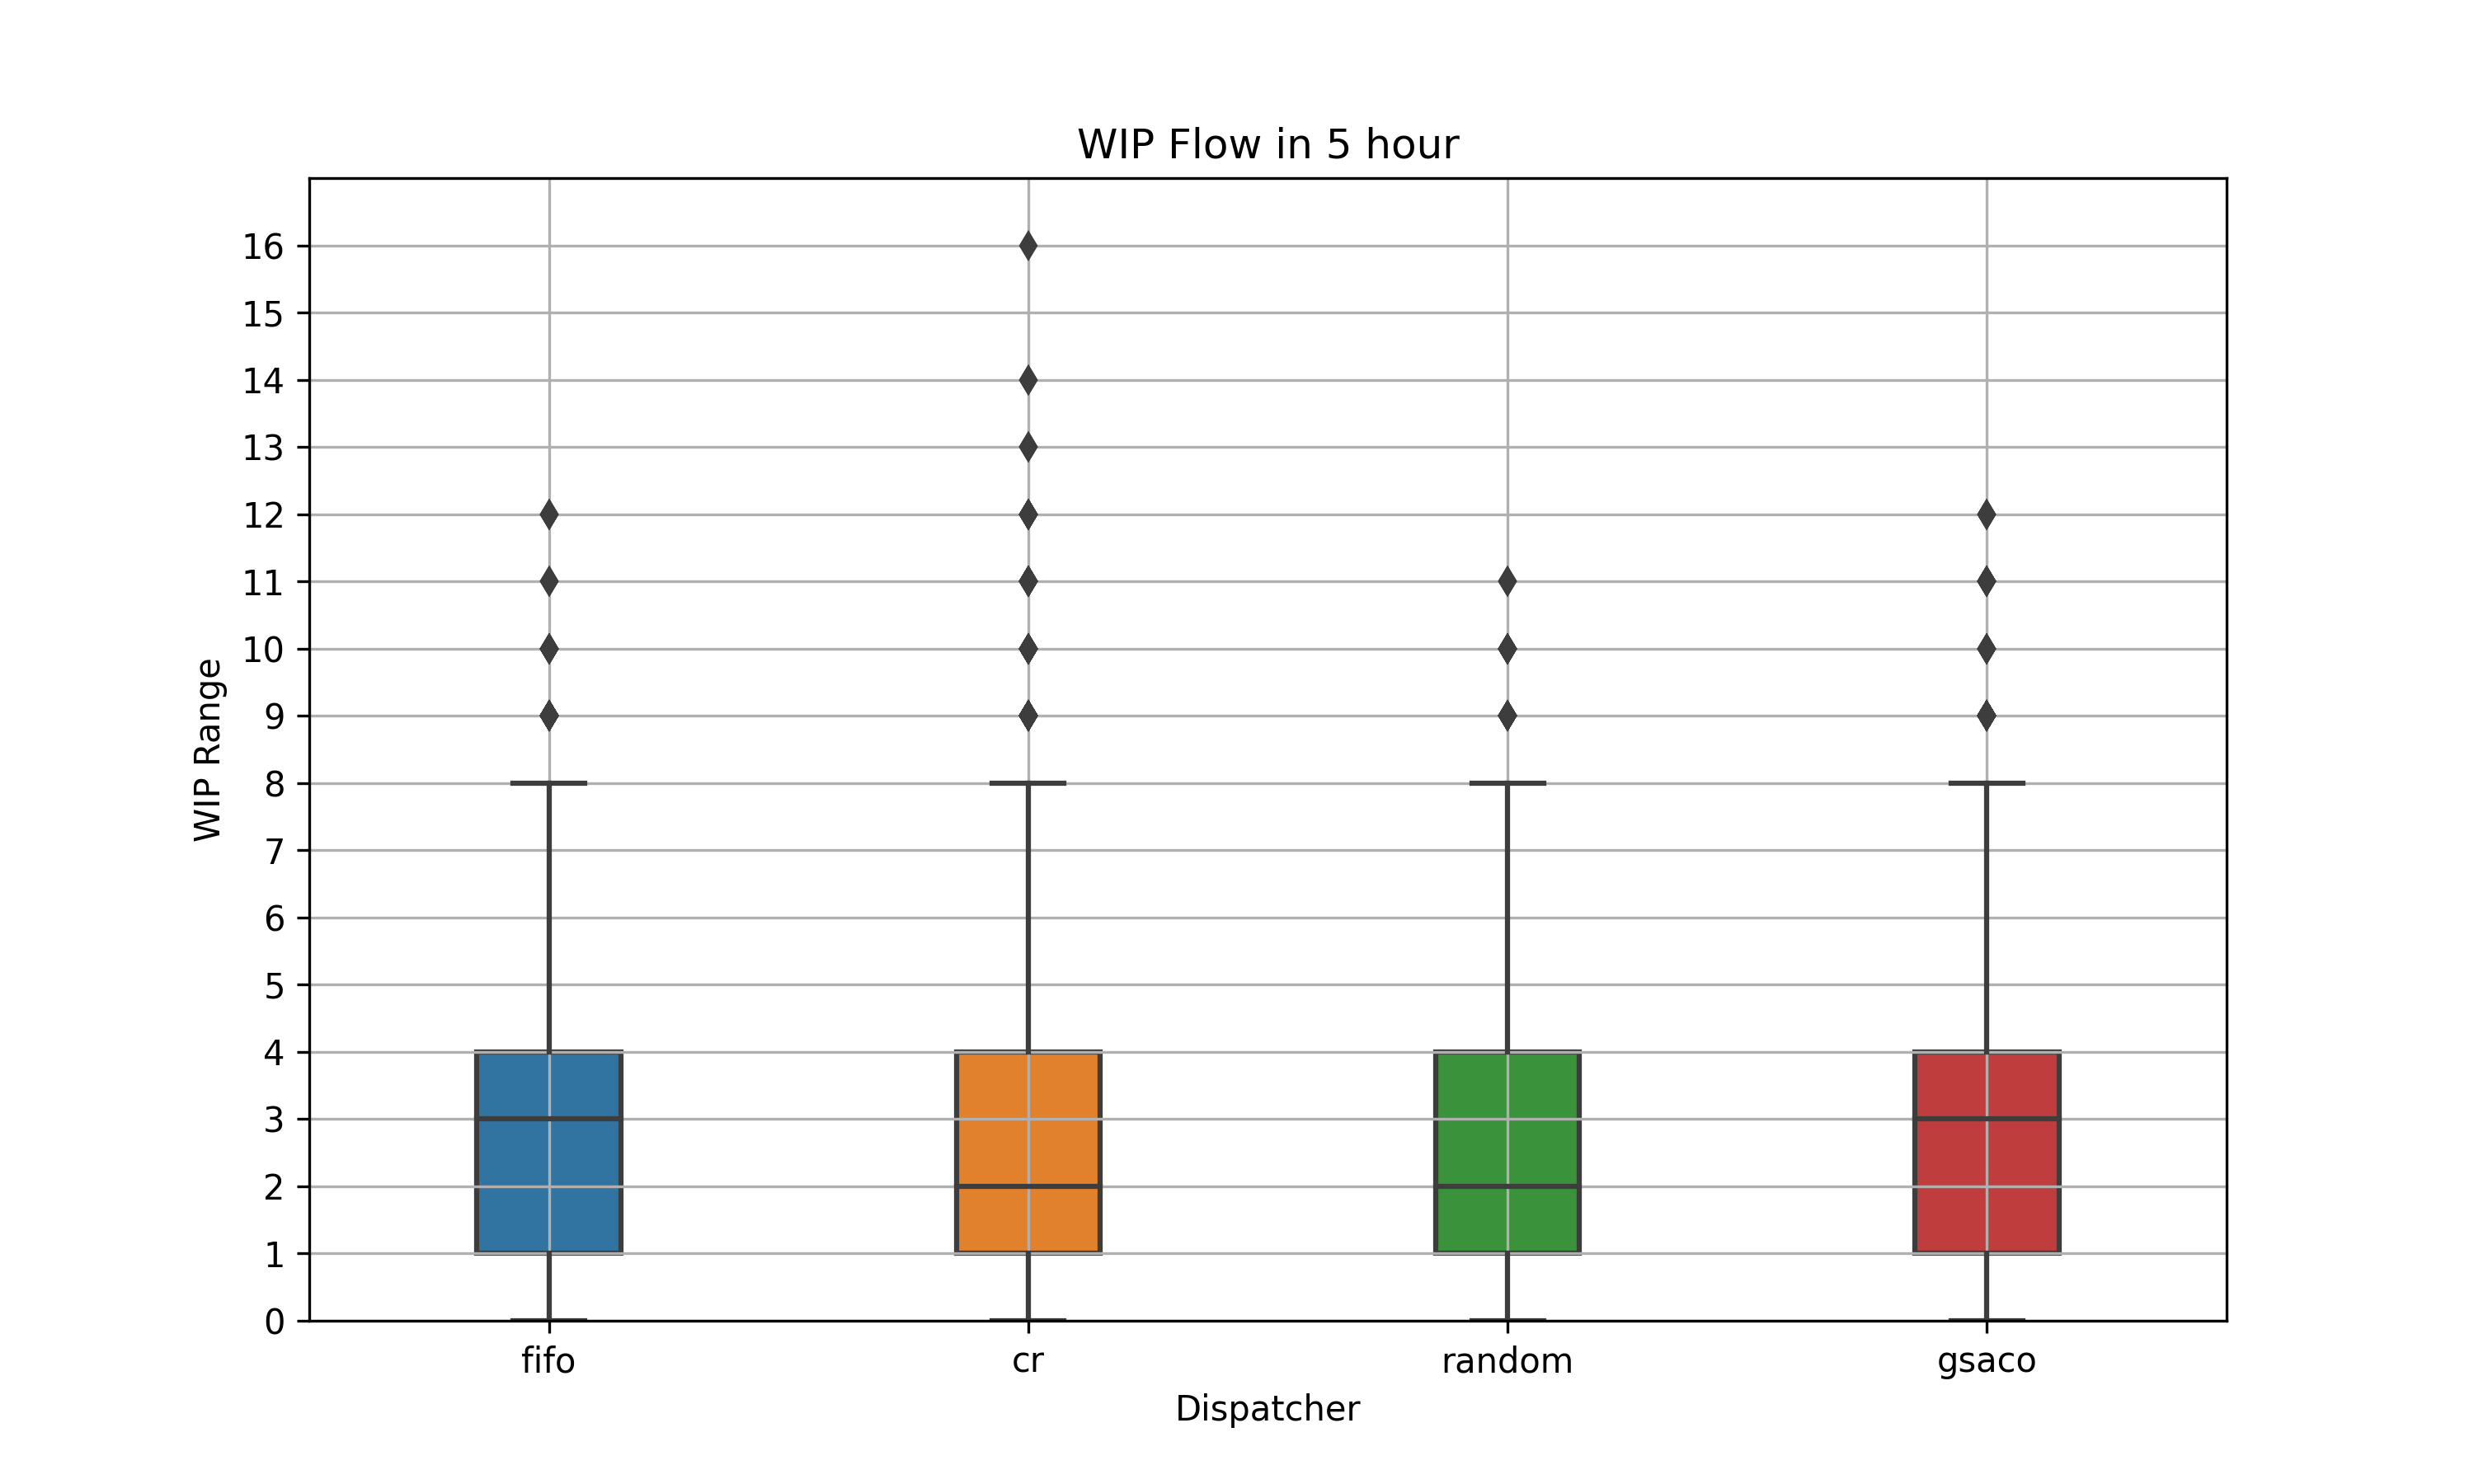
\includegraphics[width=\textwidth]{HVLM/period_18000s.png}
		% \caption{}
		% \label{fig:p5}
	\end{subfigure}
	\hfill
	\begin{subfigure}[b]{0.32\textwidth}
		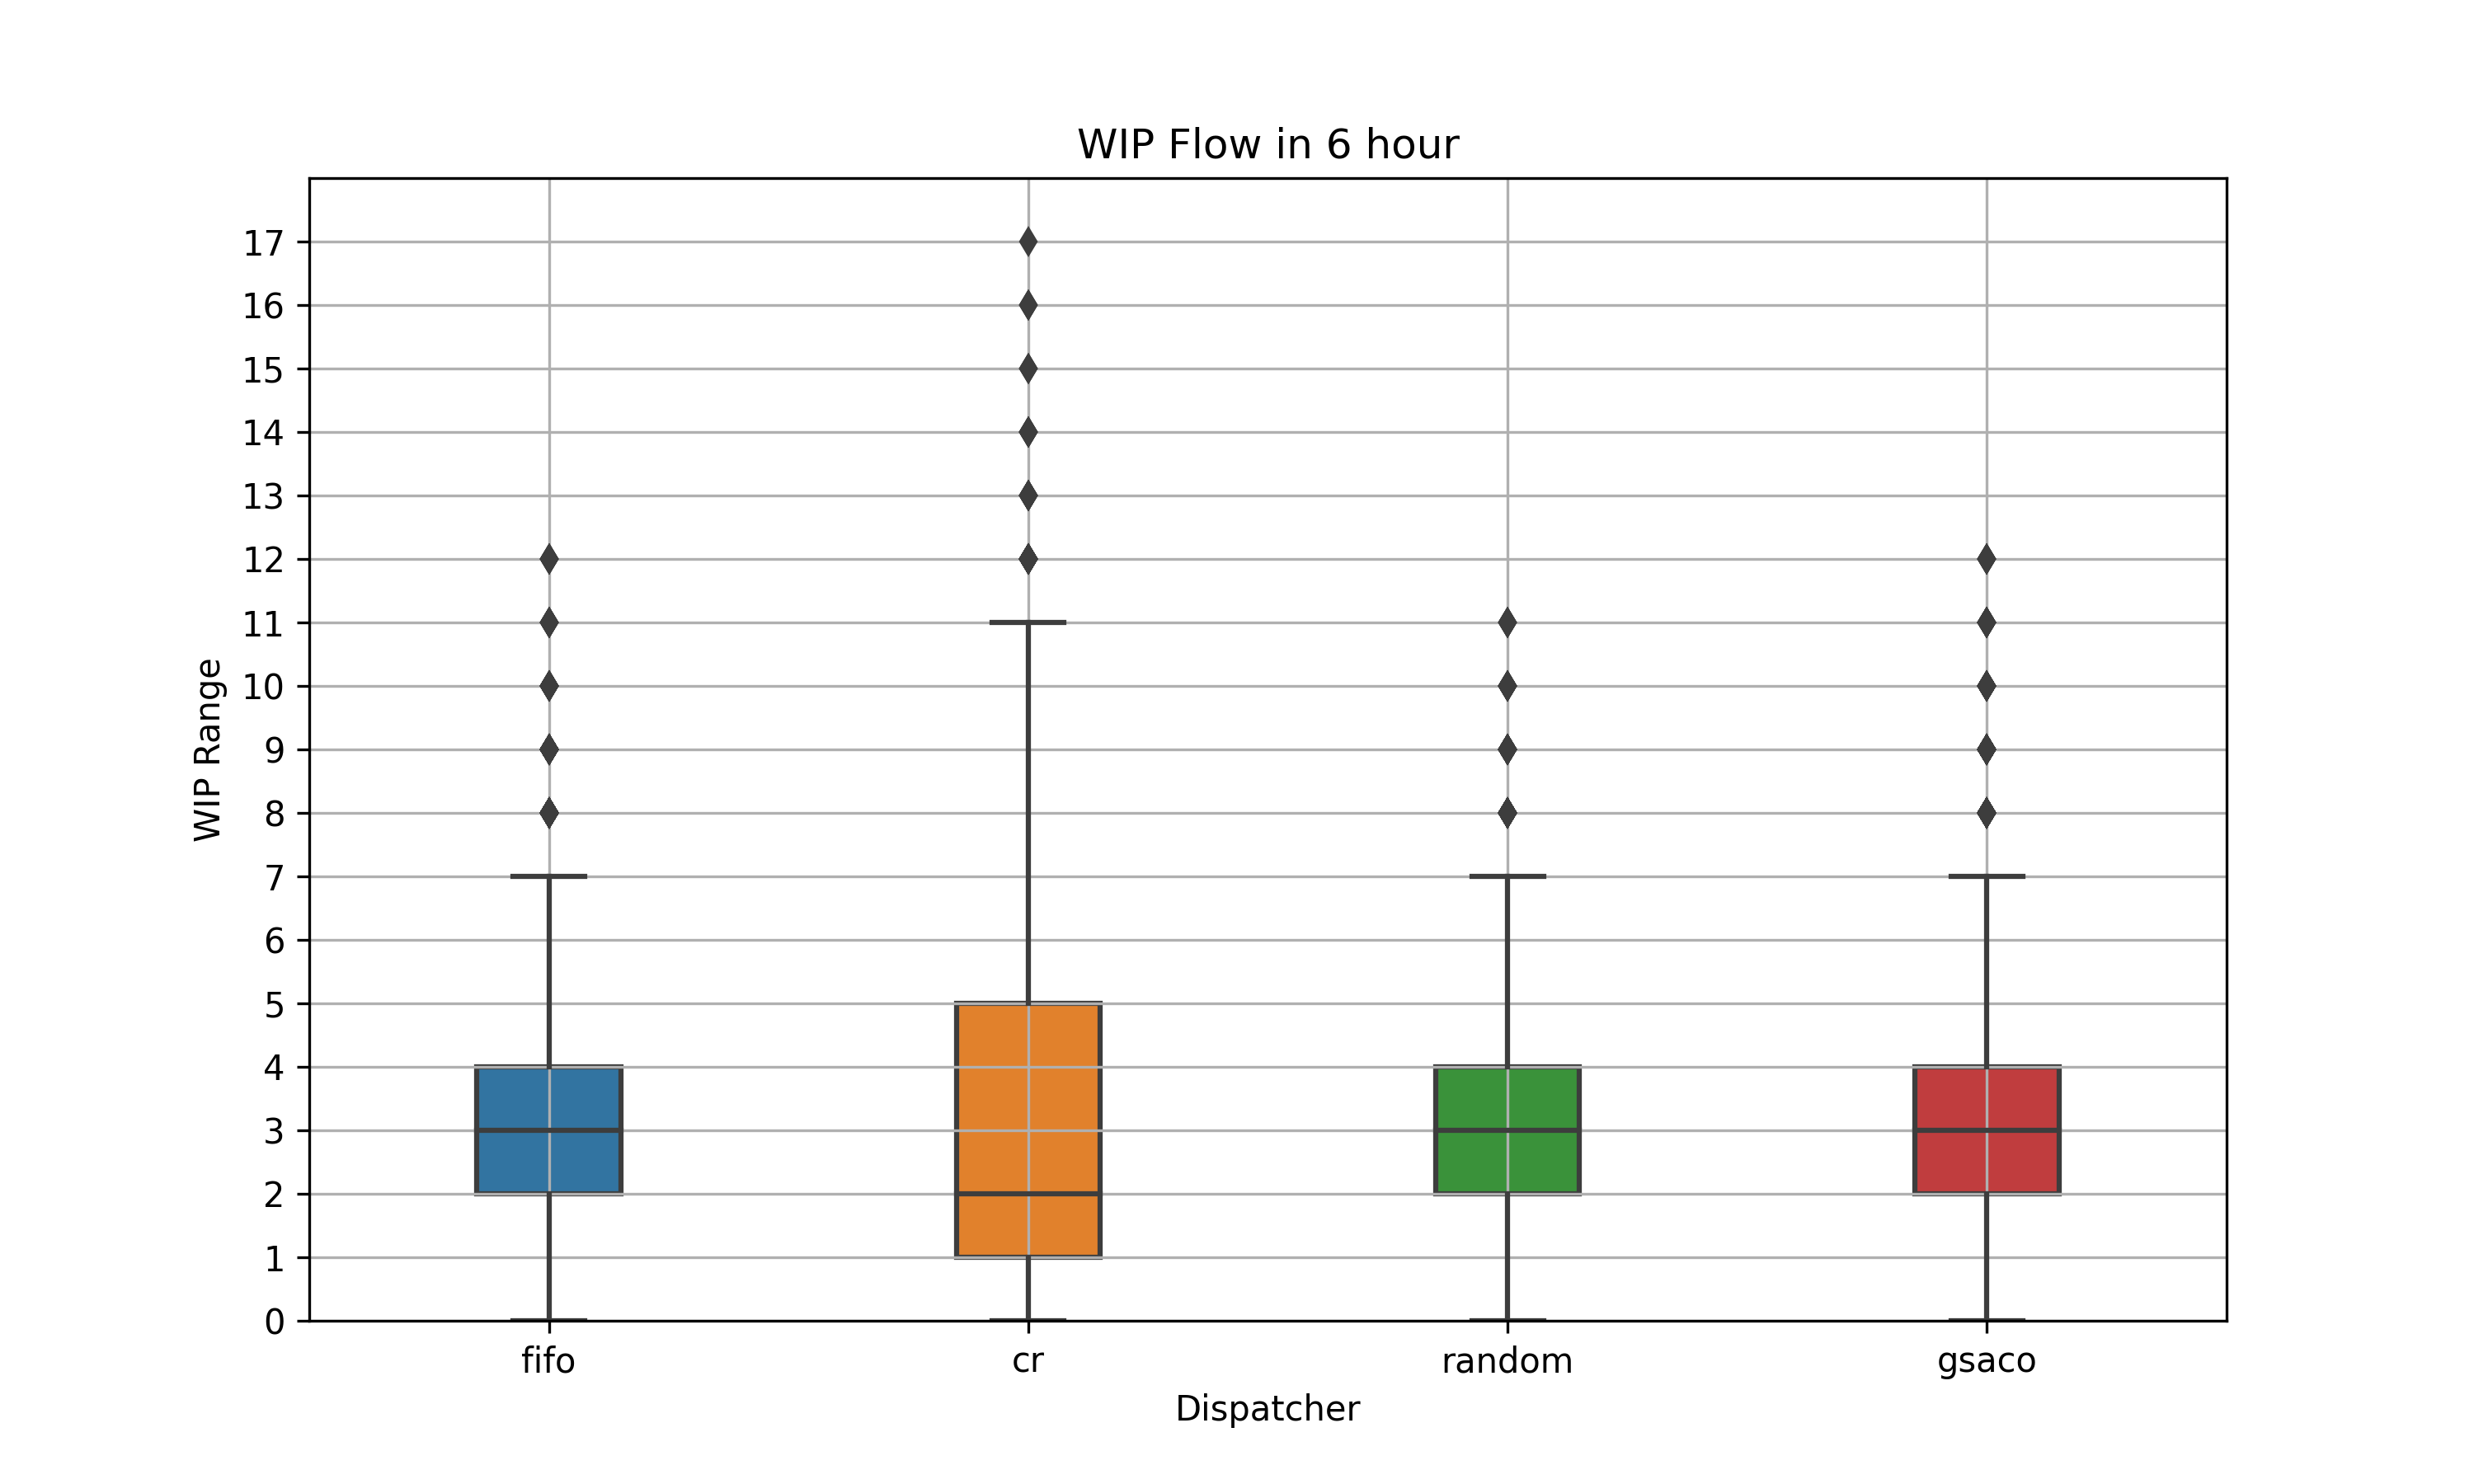
\includegraphics[width=\textwidth]{HVLM/period_21600s.png}
		% \caption{}
		% \label{fig:p6}
	\end{subfigure}
	\caption{WIP flow for HV/LM}
	\label{fig:wip-flows-HVLM}
\end{figure}

The plots in Figure~\ref{fig:totalopsHVLM} presents the performance of various dispatching rules—FIFO, CR, RANDOM, and GSACO—across different planning horizons ranging from 1 to 6 hours. Each plot illustrates the total number of operations dispatched by each rule within these time frames, offering a clear comparison of their efficiency and effectiveness in handling operational tasks within a semiconductor manufacturing.
\todo{M: Please unify the range of the $y$-scales in subfigures of each of the Figures~\ref{fig:totalopsHVLM}--\ref{fig:totalopsLVHM}.}

The performance of dispatching rules based on specific operational times and goals are analyzed. While simpler rules like FIFO and CR are predictable and may perform adequately in stable environments, their performance can lag in more dynamic or complex scenarios where adaptive strategies like GSACO provide significant advantages. Random dispatching, surprisingly effective in some cases, suggests that stochastic elements might occasionally align with operational demands, although this method's reliability is less consistent. GSACO's consistently superior performance advocates for its use in environments where maximizing operational throughput is critical. This analysis not only aids in strategic decision-making but also highlights the potential for further refining these algorithms to enhance their applicability and effectiveness across various manufacturing contexts.

The plots in Figure~\ref{fig:wip-flows-HVLM} illustrate the Work in Progress (WIP) flow across various dispatching rules—FIFO, CR, RANDOM, and GSACO —over different planning horizons ranging from 1 to 6 hours. Each bar demonstrates the minimum and maximum WIP levels reached during the simulation period under each dispatching rule, with the height of the bar indicating the variability or stability of the WIP flow.

FIFO shows the lowest range of WIP variability, suggesting consistent and predictable processing under this rule within the first hour. CR and Random display slightly higher variability, indicating a less stable WIP flow.
GSACO exhibits the highest range, potentially due to more aggressive reordering and optimization strategies that initially increase variability before stabilizing.

As the planning horizon extends to 2, 3, 4, 5, and 6 hours, all methods show an increase in the maximum WIP range. FIFO consistently maintains a relatively lower range of WIP compared to other methods, indicating its less dynamic but stable approach.
CR's performance exhibits moderate variability, reflecting its strategy of prioritizing jobs based on their deadlines, which might not always align with minimizing WIP.
Random shows a moderate to high variability, which aligns with its inherent unpredictability.
GSACO consistently demonstrates the highest variability. This could be attributed to its optimization processes, which might involve significant shifts in job prioritization and scheduling to achieve long-term efficiency, leading to larger fluctuations in WIP.

\begin{figure}[t]
	\centering
	\begin{subfigure}{0.32\textwidth}
		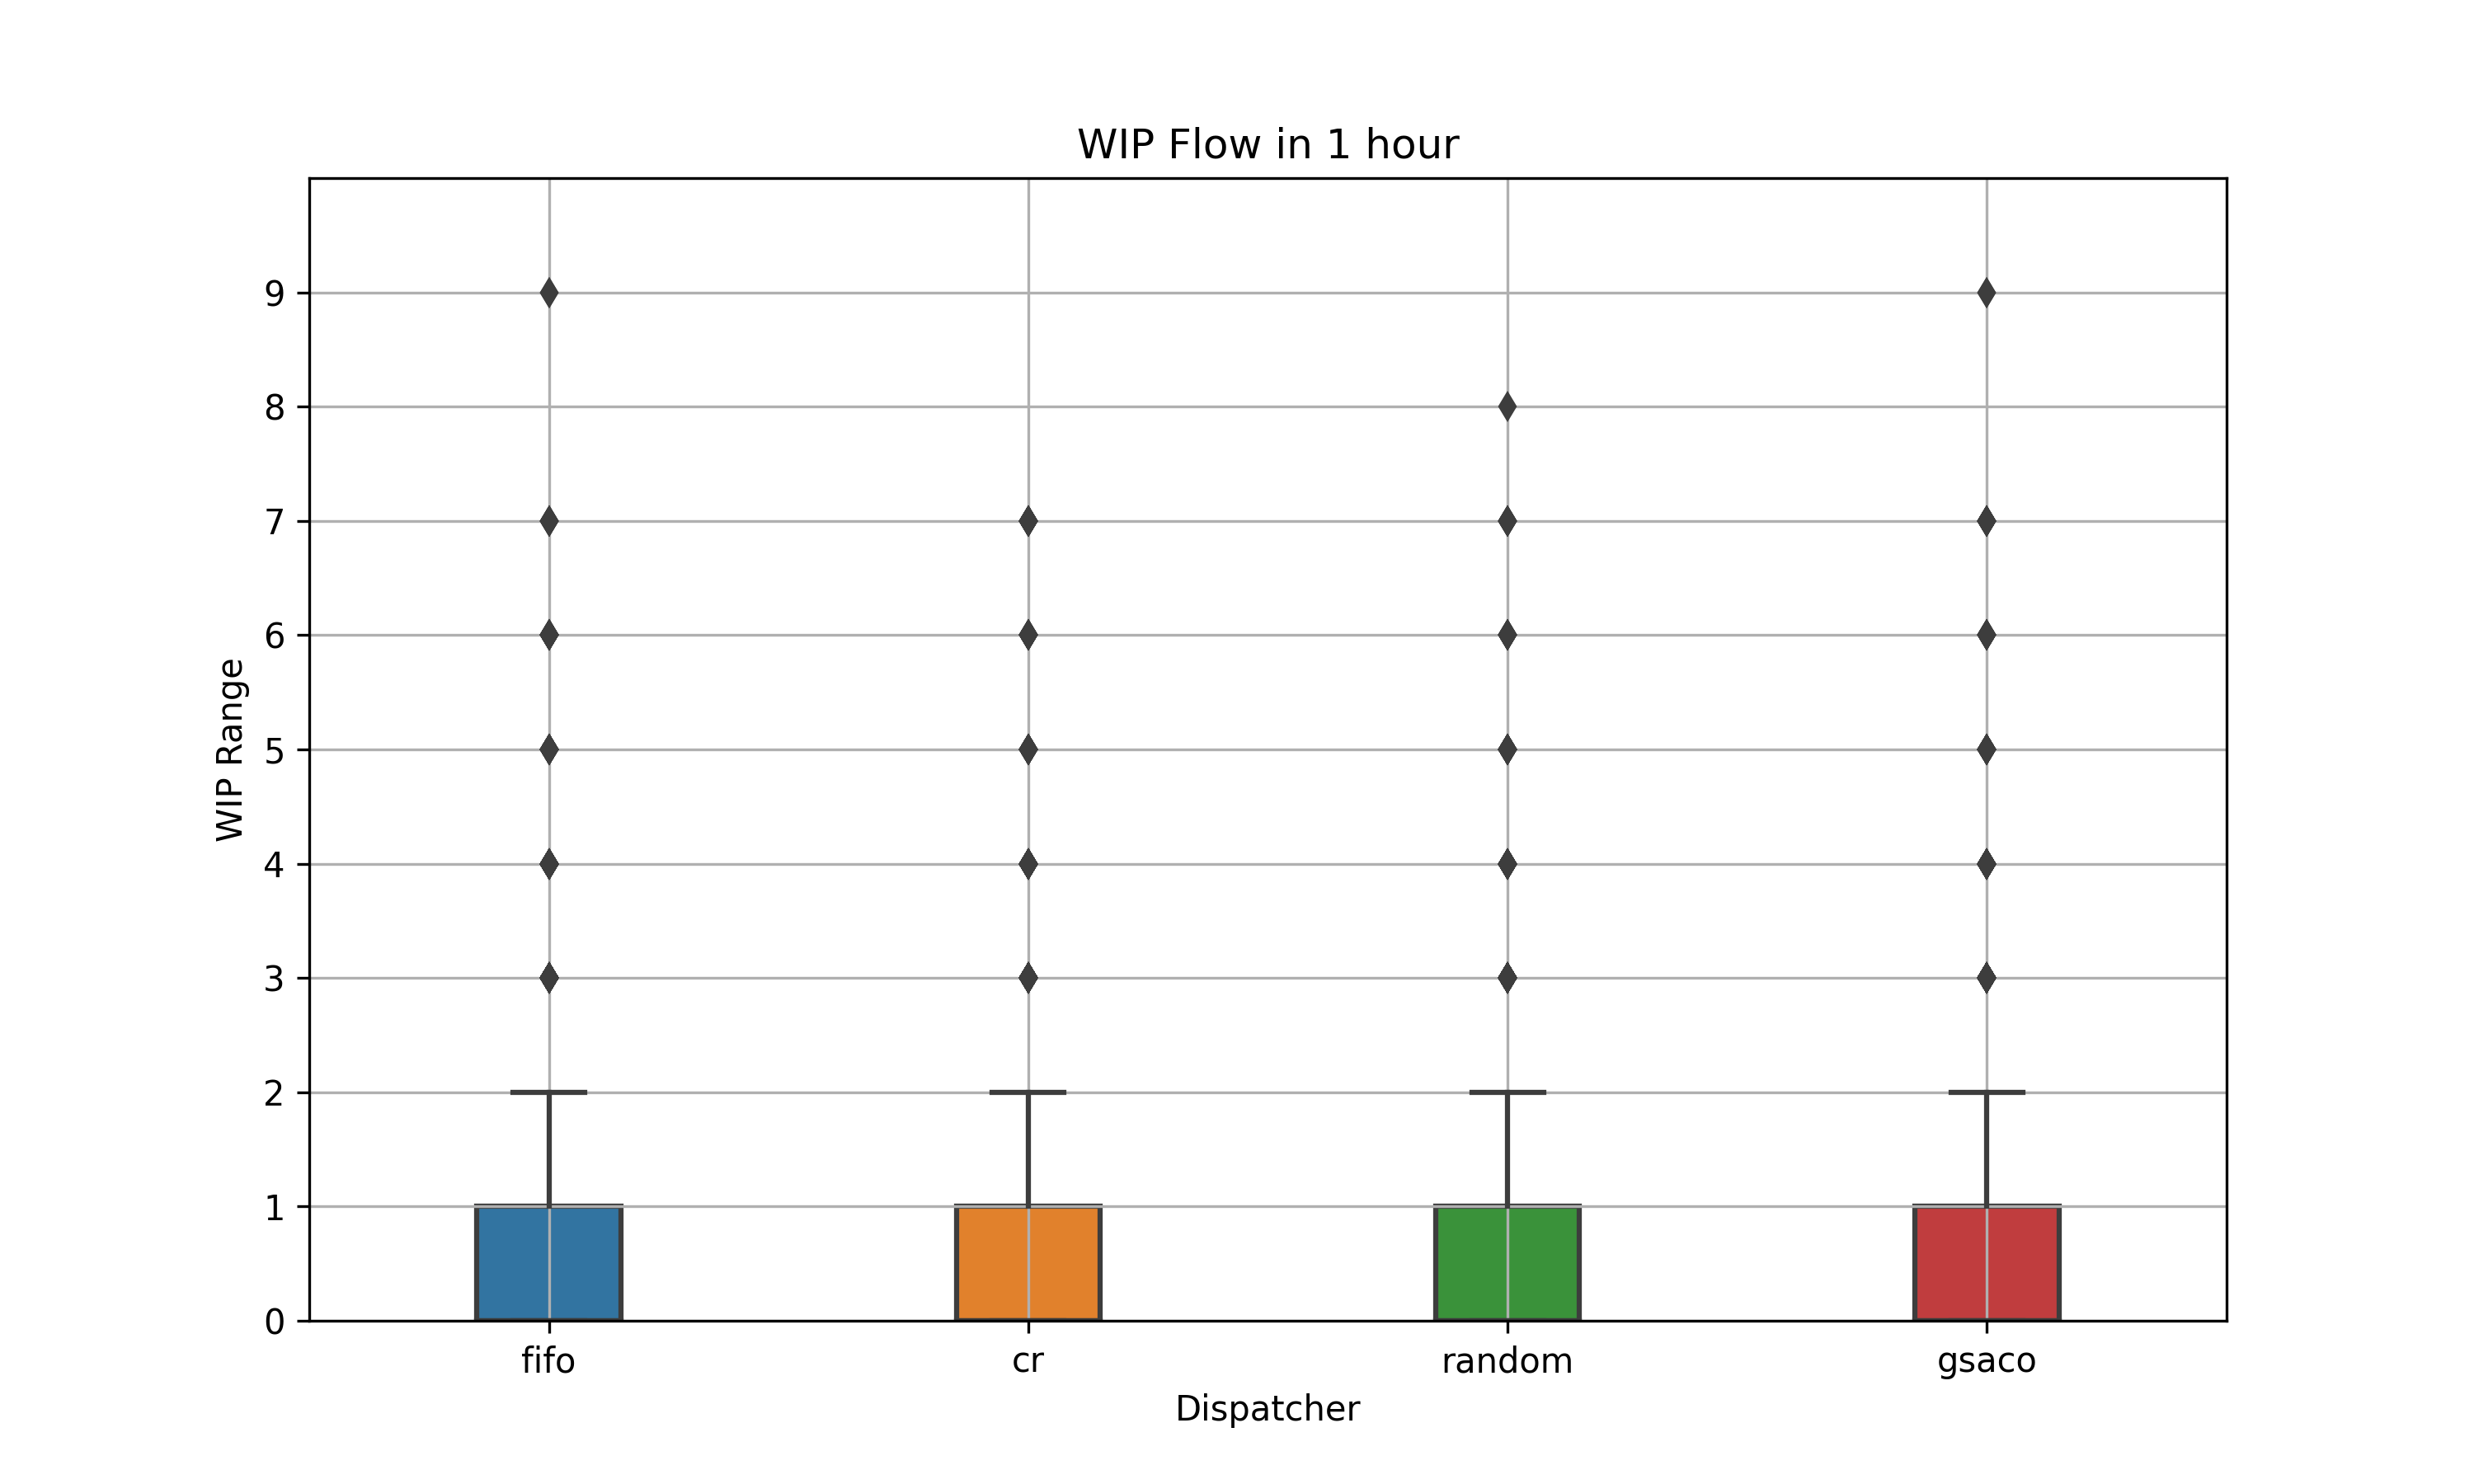
\includegraphics[width=\textwidth]{LVHM/period_3600s.png}
		% \caption{}
		% \label{fig:pp1}
	\end{subfigure}\hfill
	\begin{subfigure}{0.32\textwidth}
		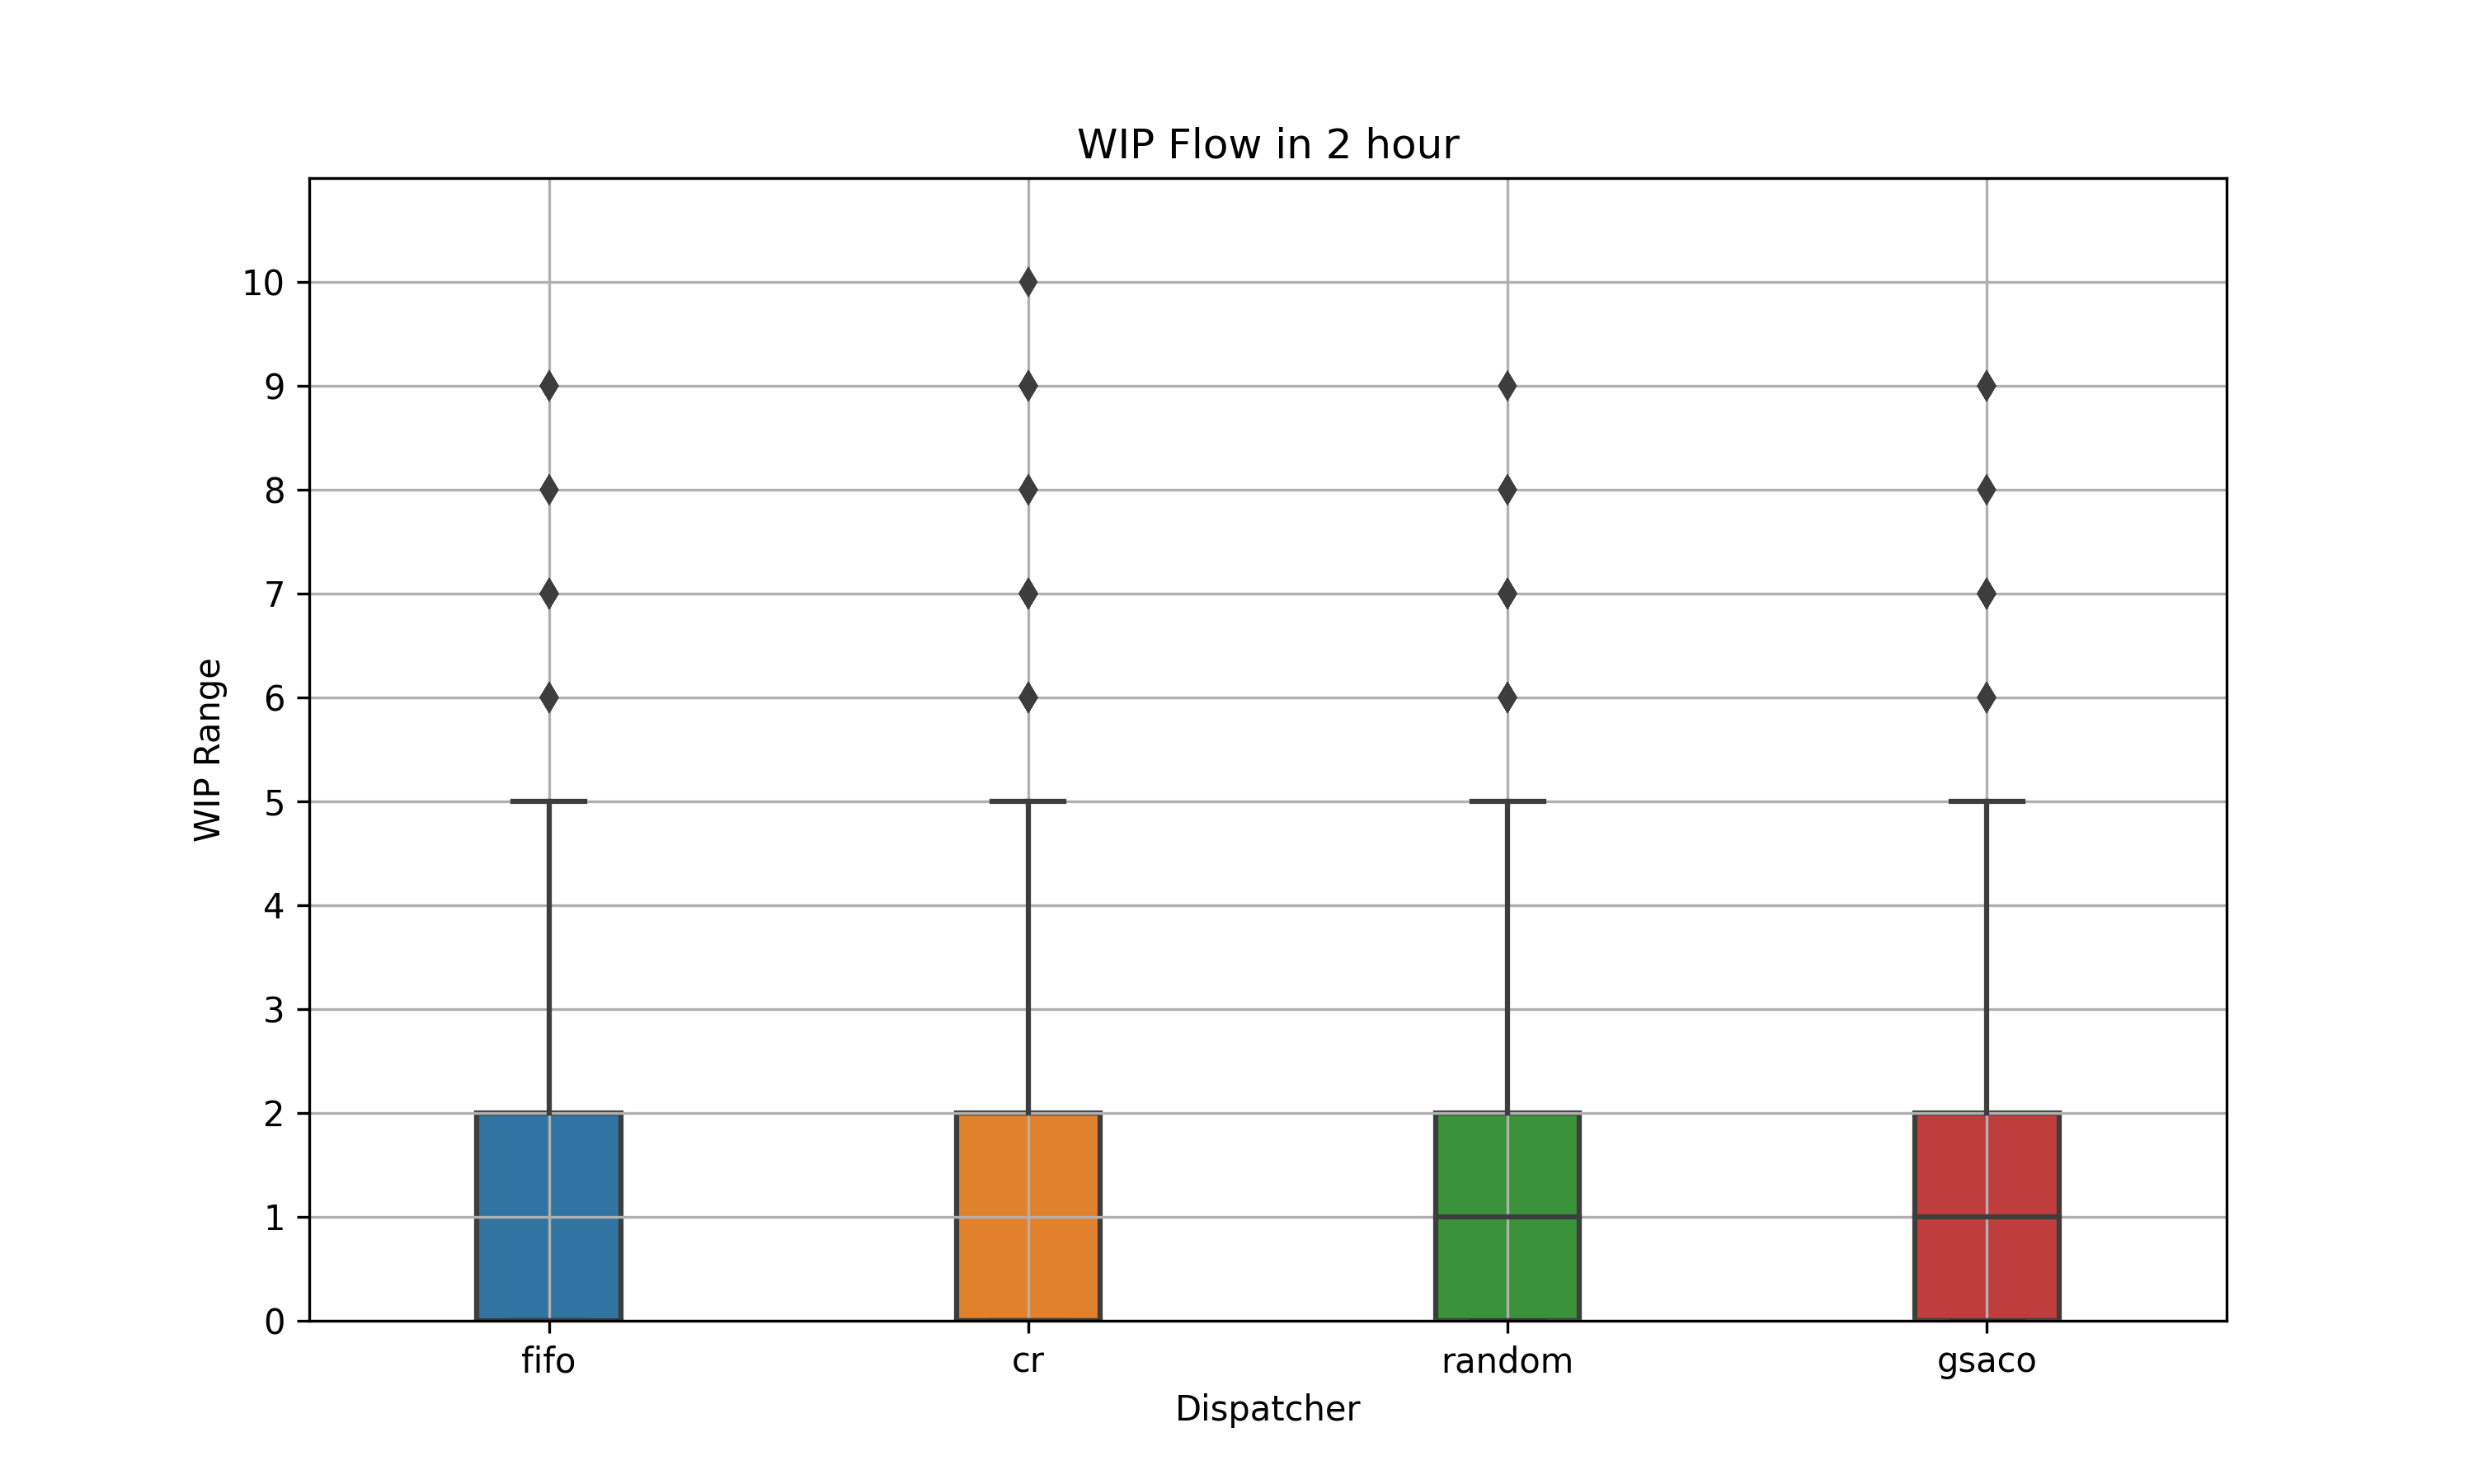
\includegraphics[width=\textwidth]{LVHM/period_7200s.png}
		% \caption{}
		% \label{fig:pp2}
	\end{subfigure}\hfill
	\begin{subfigure}{0.32\textwidth}
		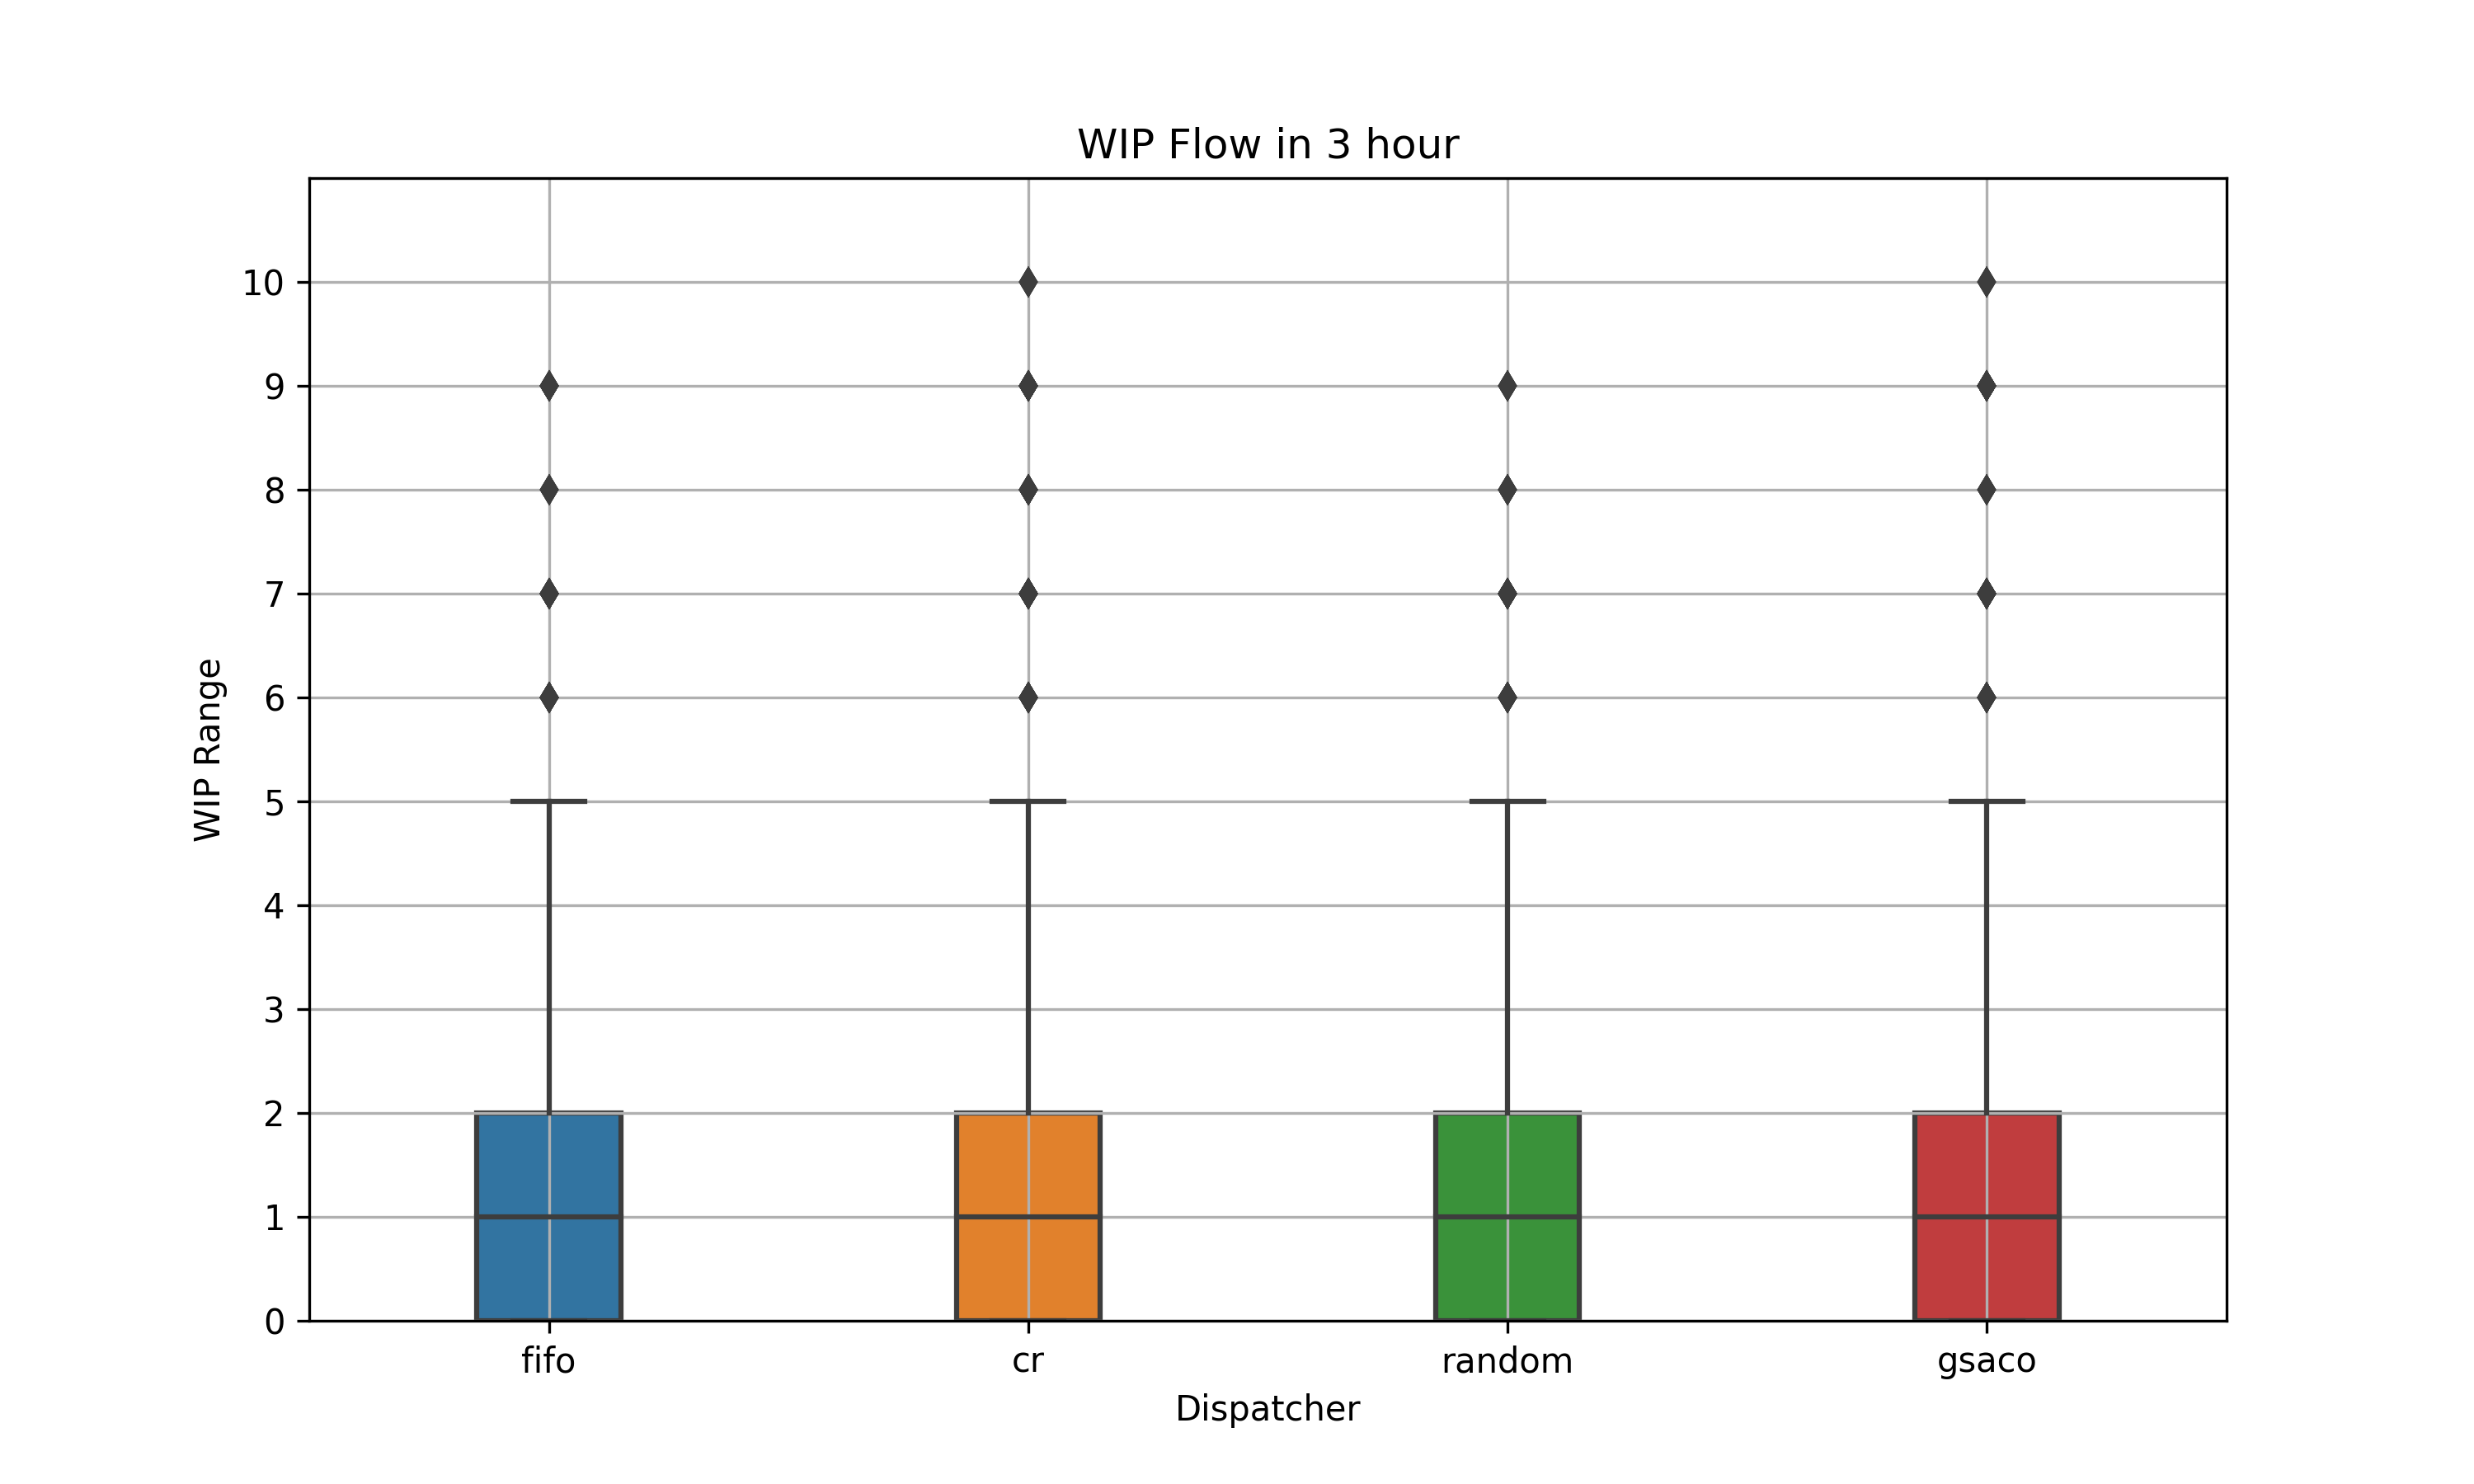
\includegraphics[width=\textwidth]{LVHM/period_10800s.png}
		% \caption{}
		% \label{fig:pp3}
	\end{subfigure}
	\begin{subfigure}{0.32\textwidth}
		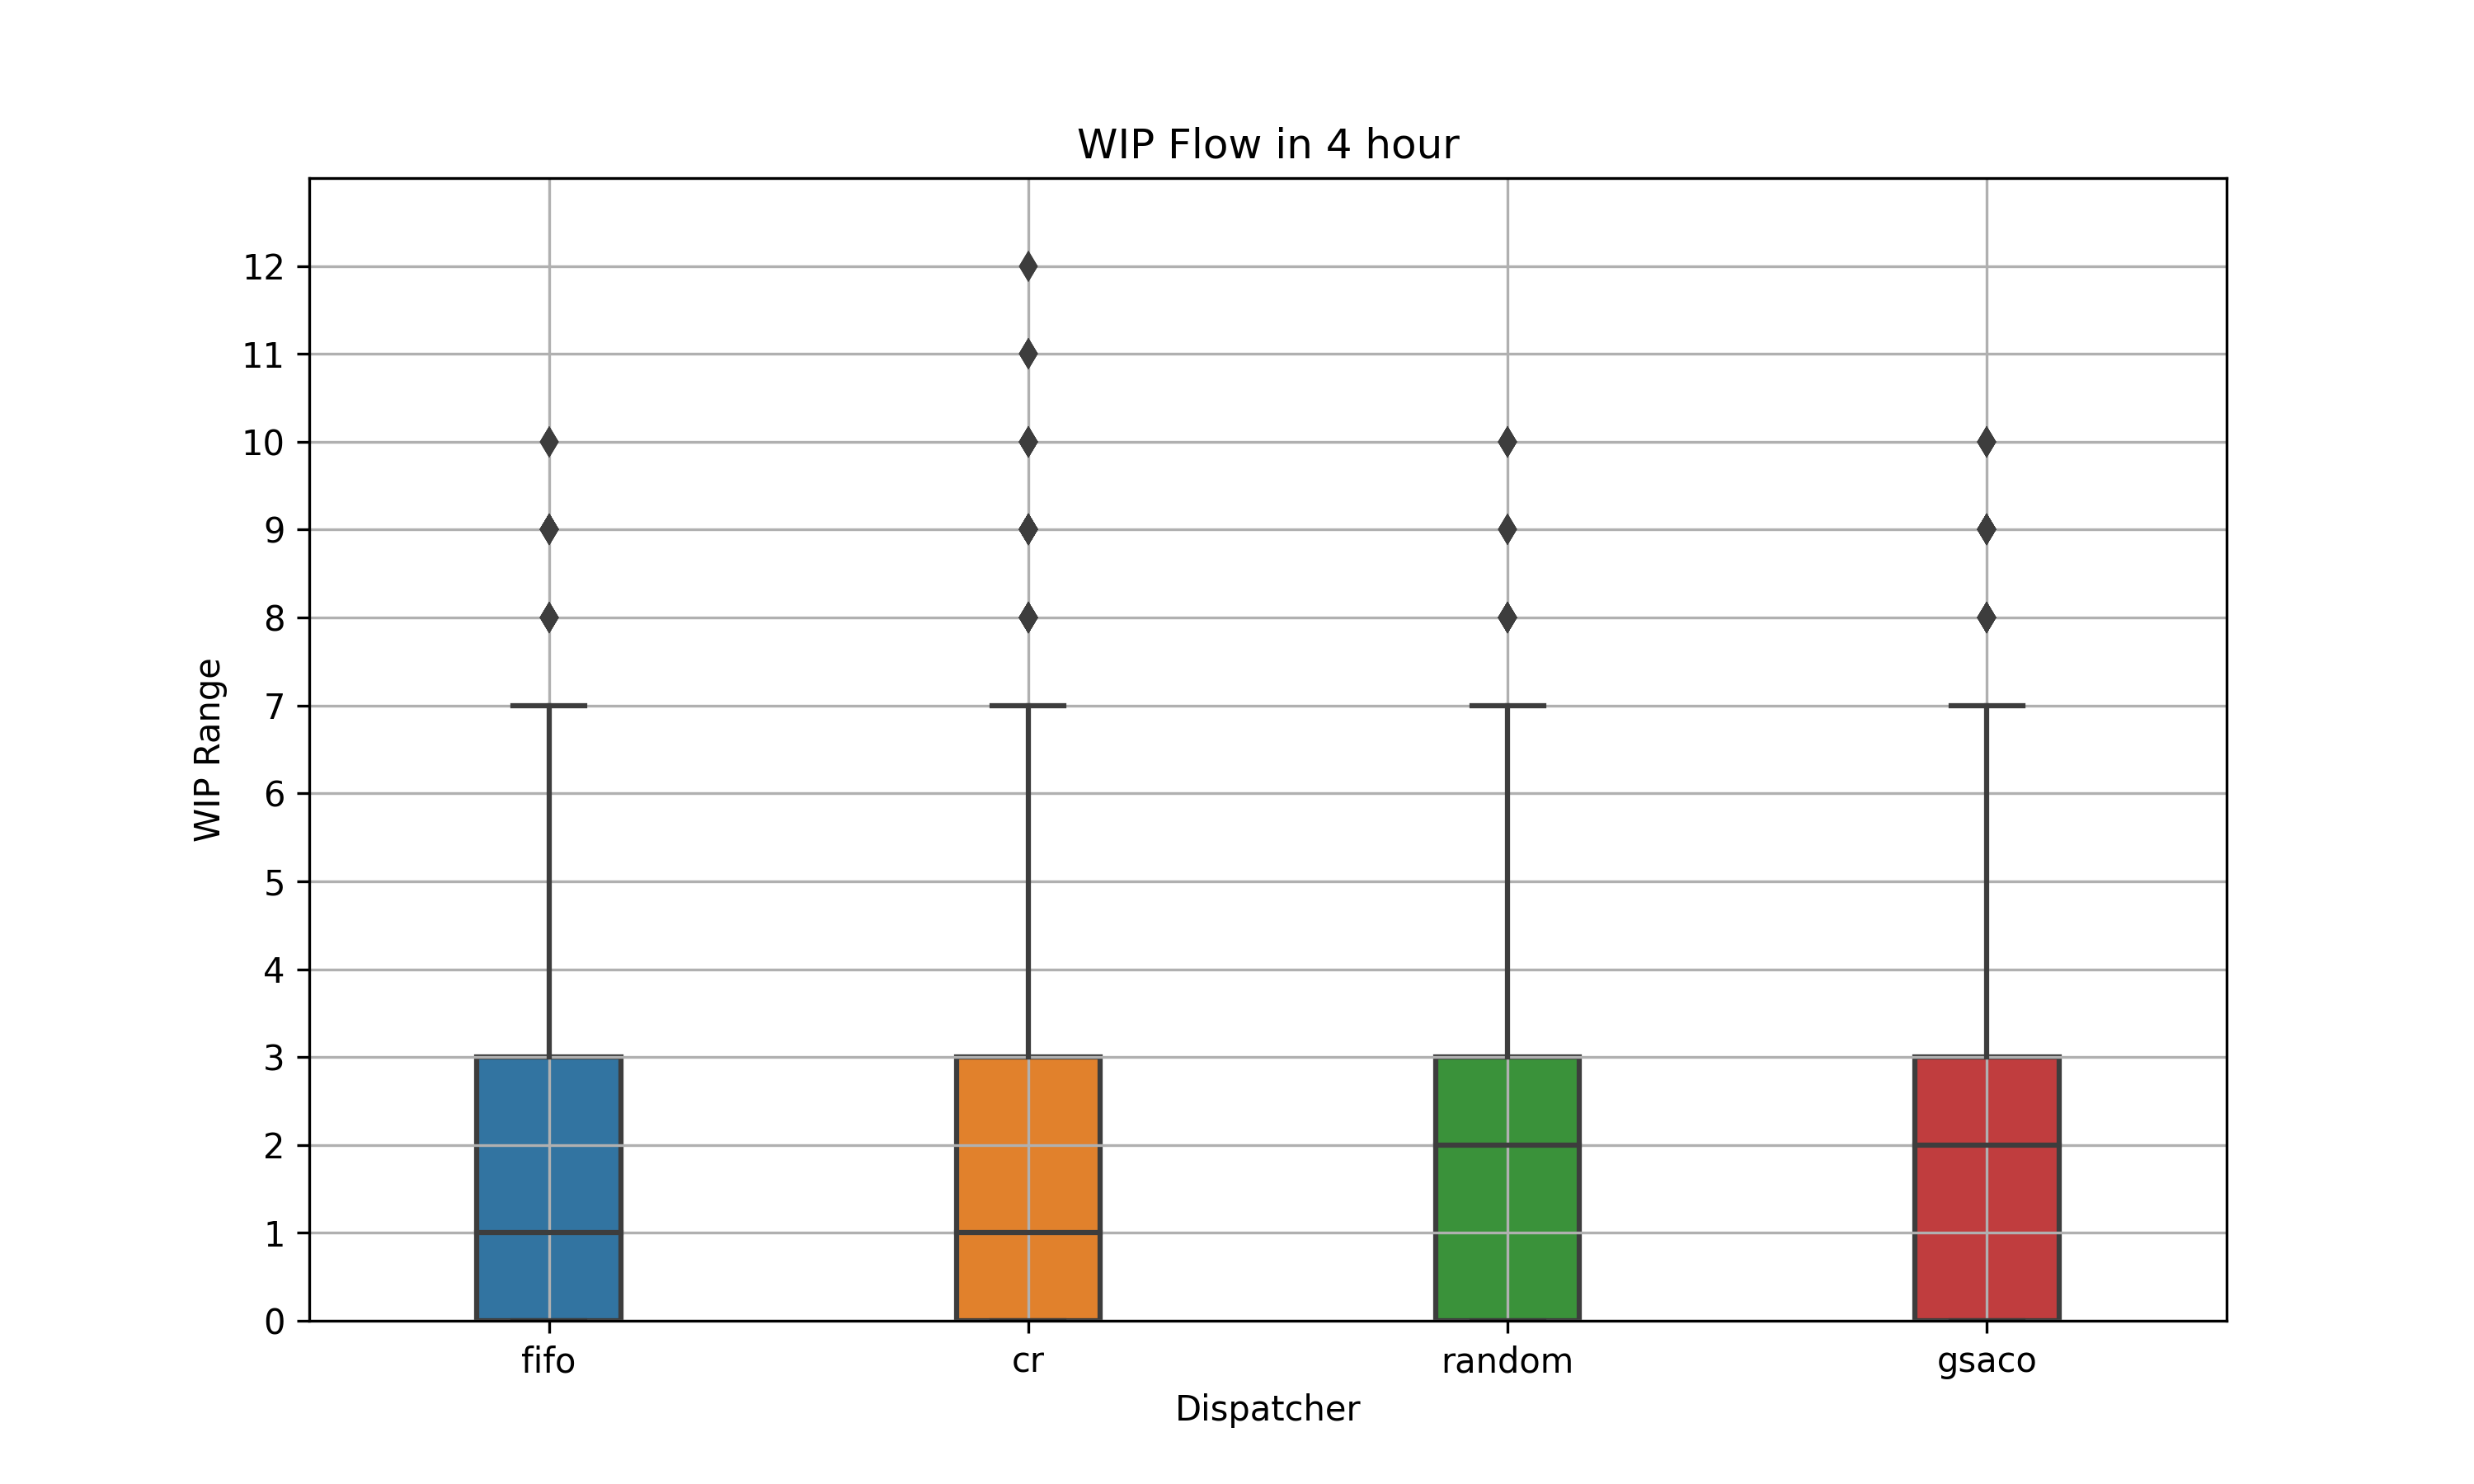
\includegraphics[width=\textwidth]{LVHM/period_14400s.png}
		% \caption{}
		% \label{fig:pp4}
	\end{subfigure}\hfill
	\begin{subfigure}{0.32\textwidth}
		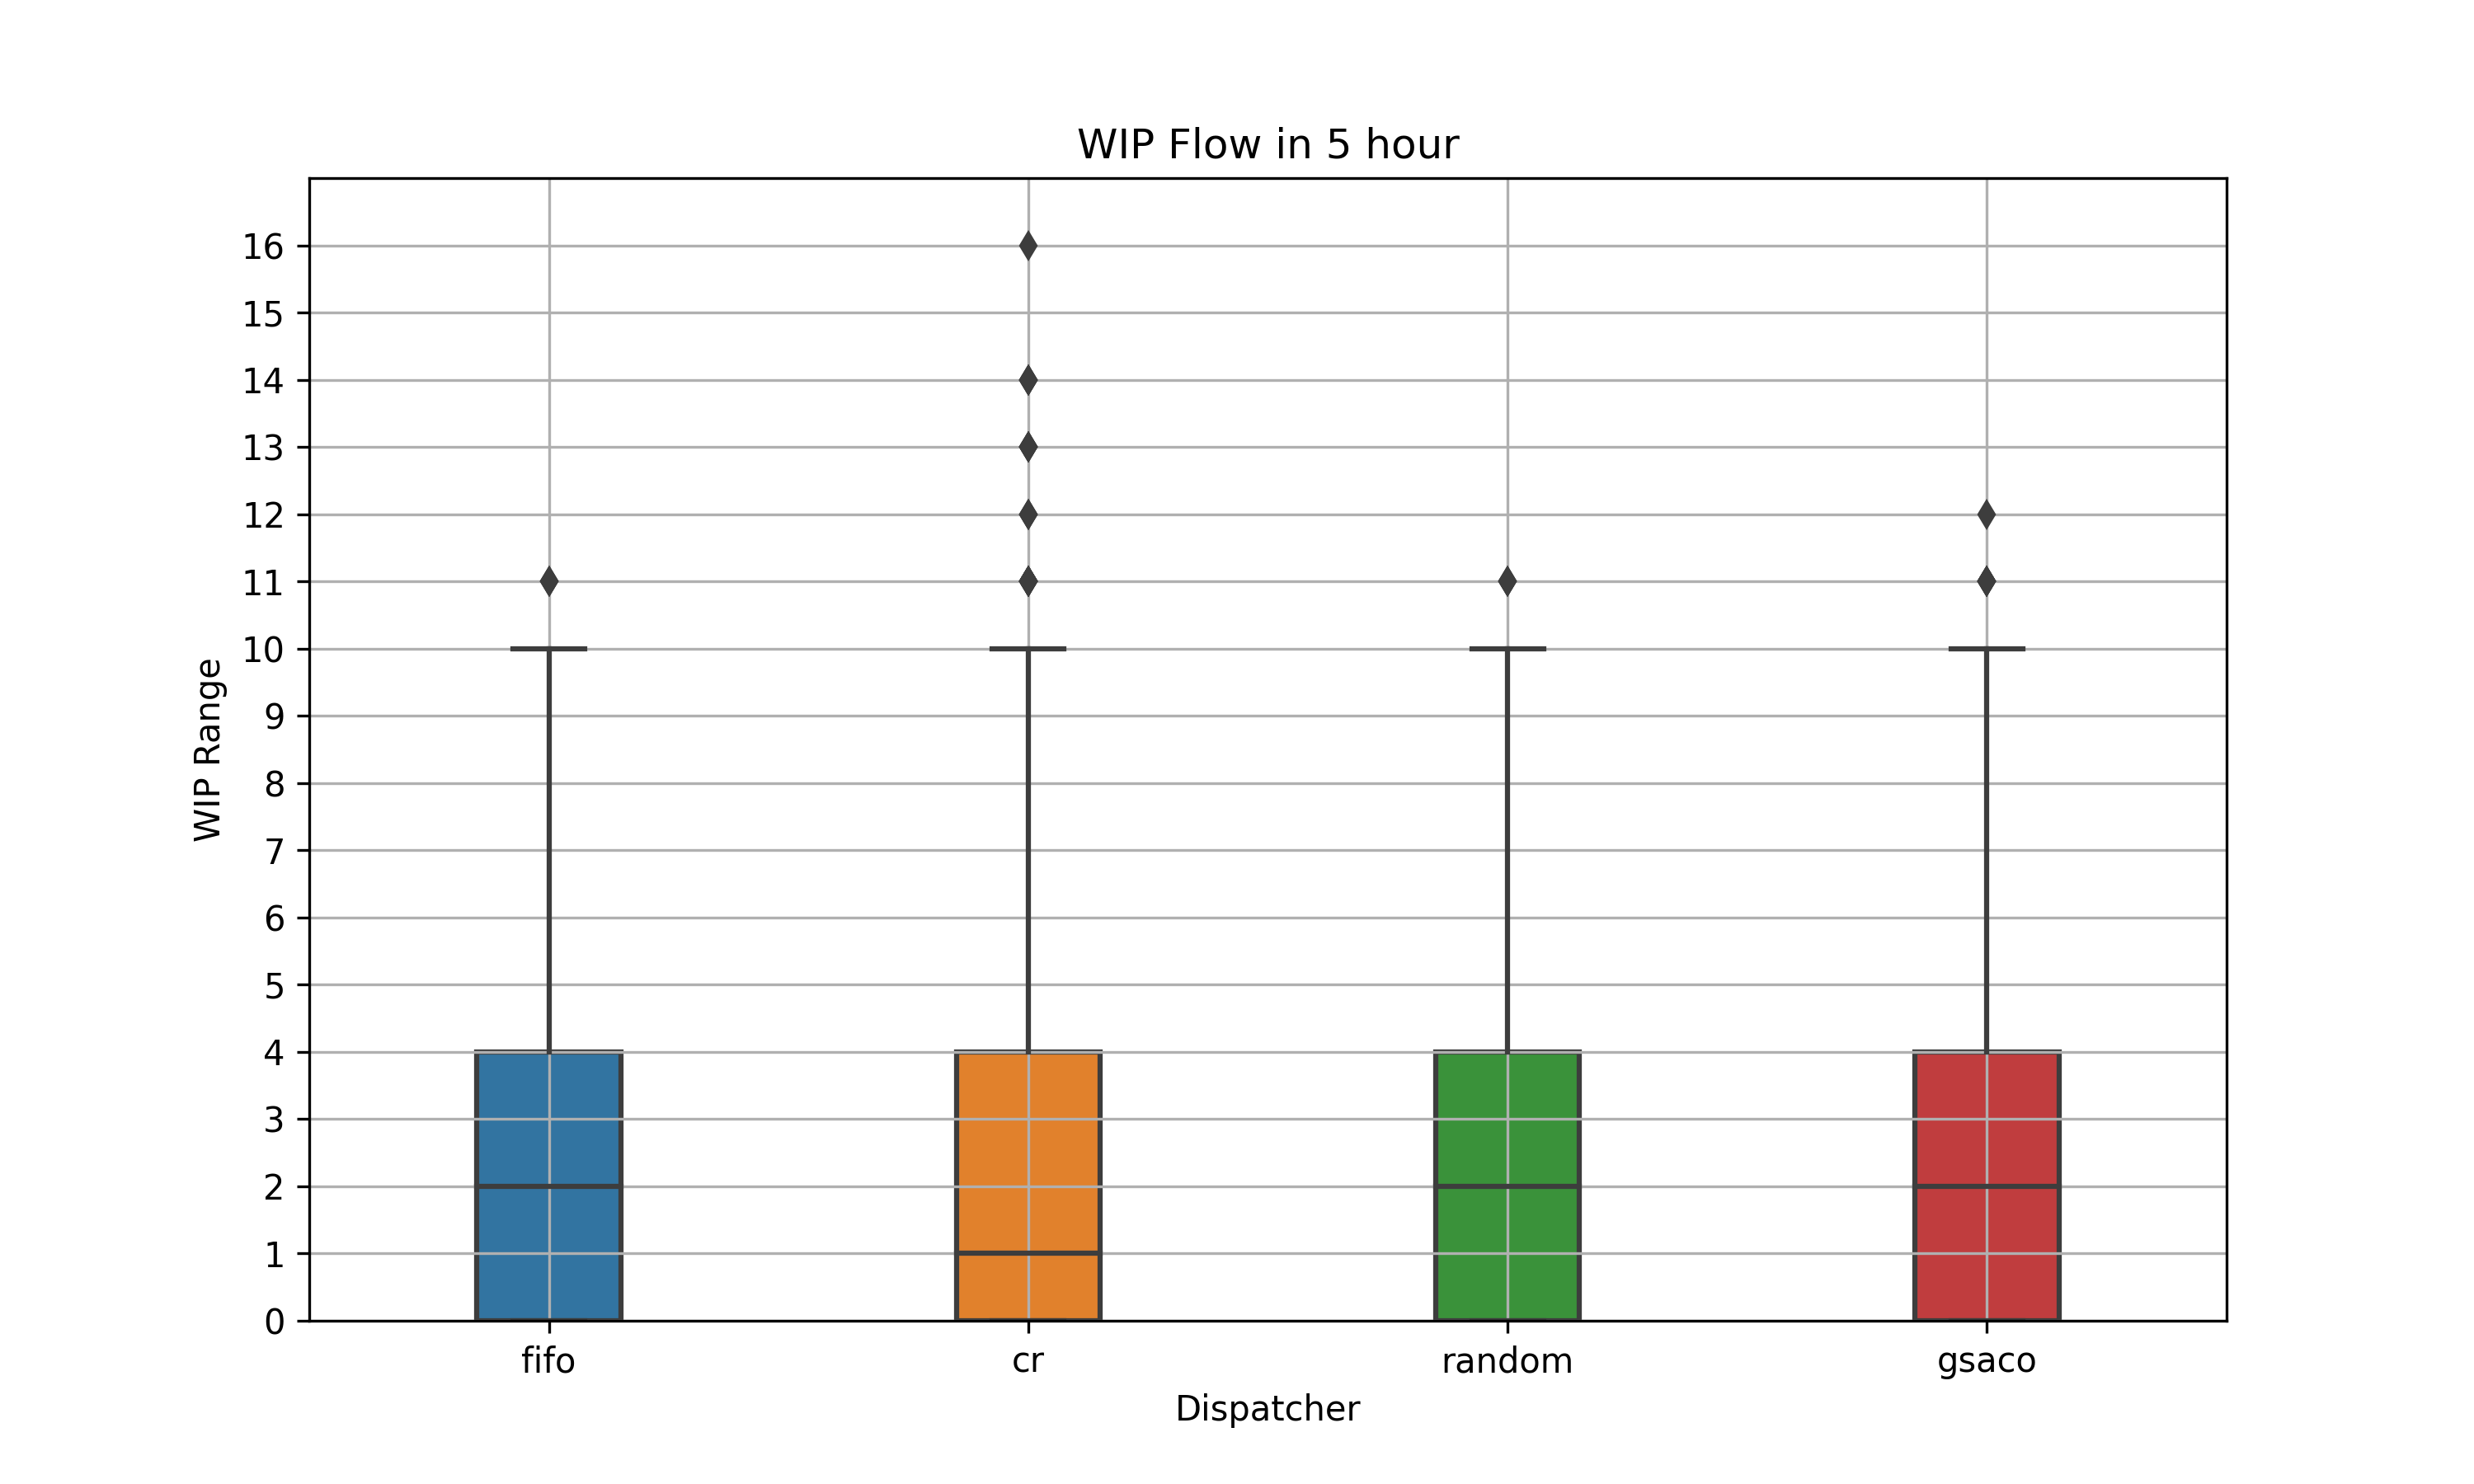
\includegraphics[width=\textwidth]{LVHM/period_18000s.png}
		% \caption{}
		% \label{fig:pp5}
	\end{subfigure}\hfill
	\begin{subfigure}{0.32\textwidth}
		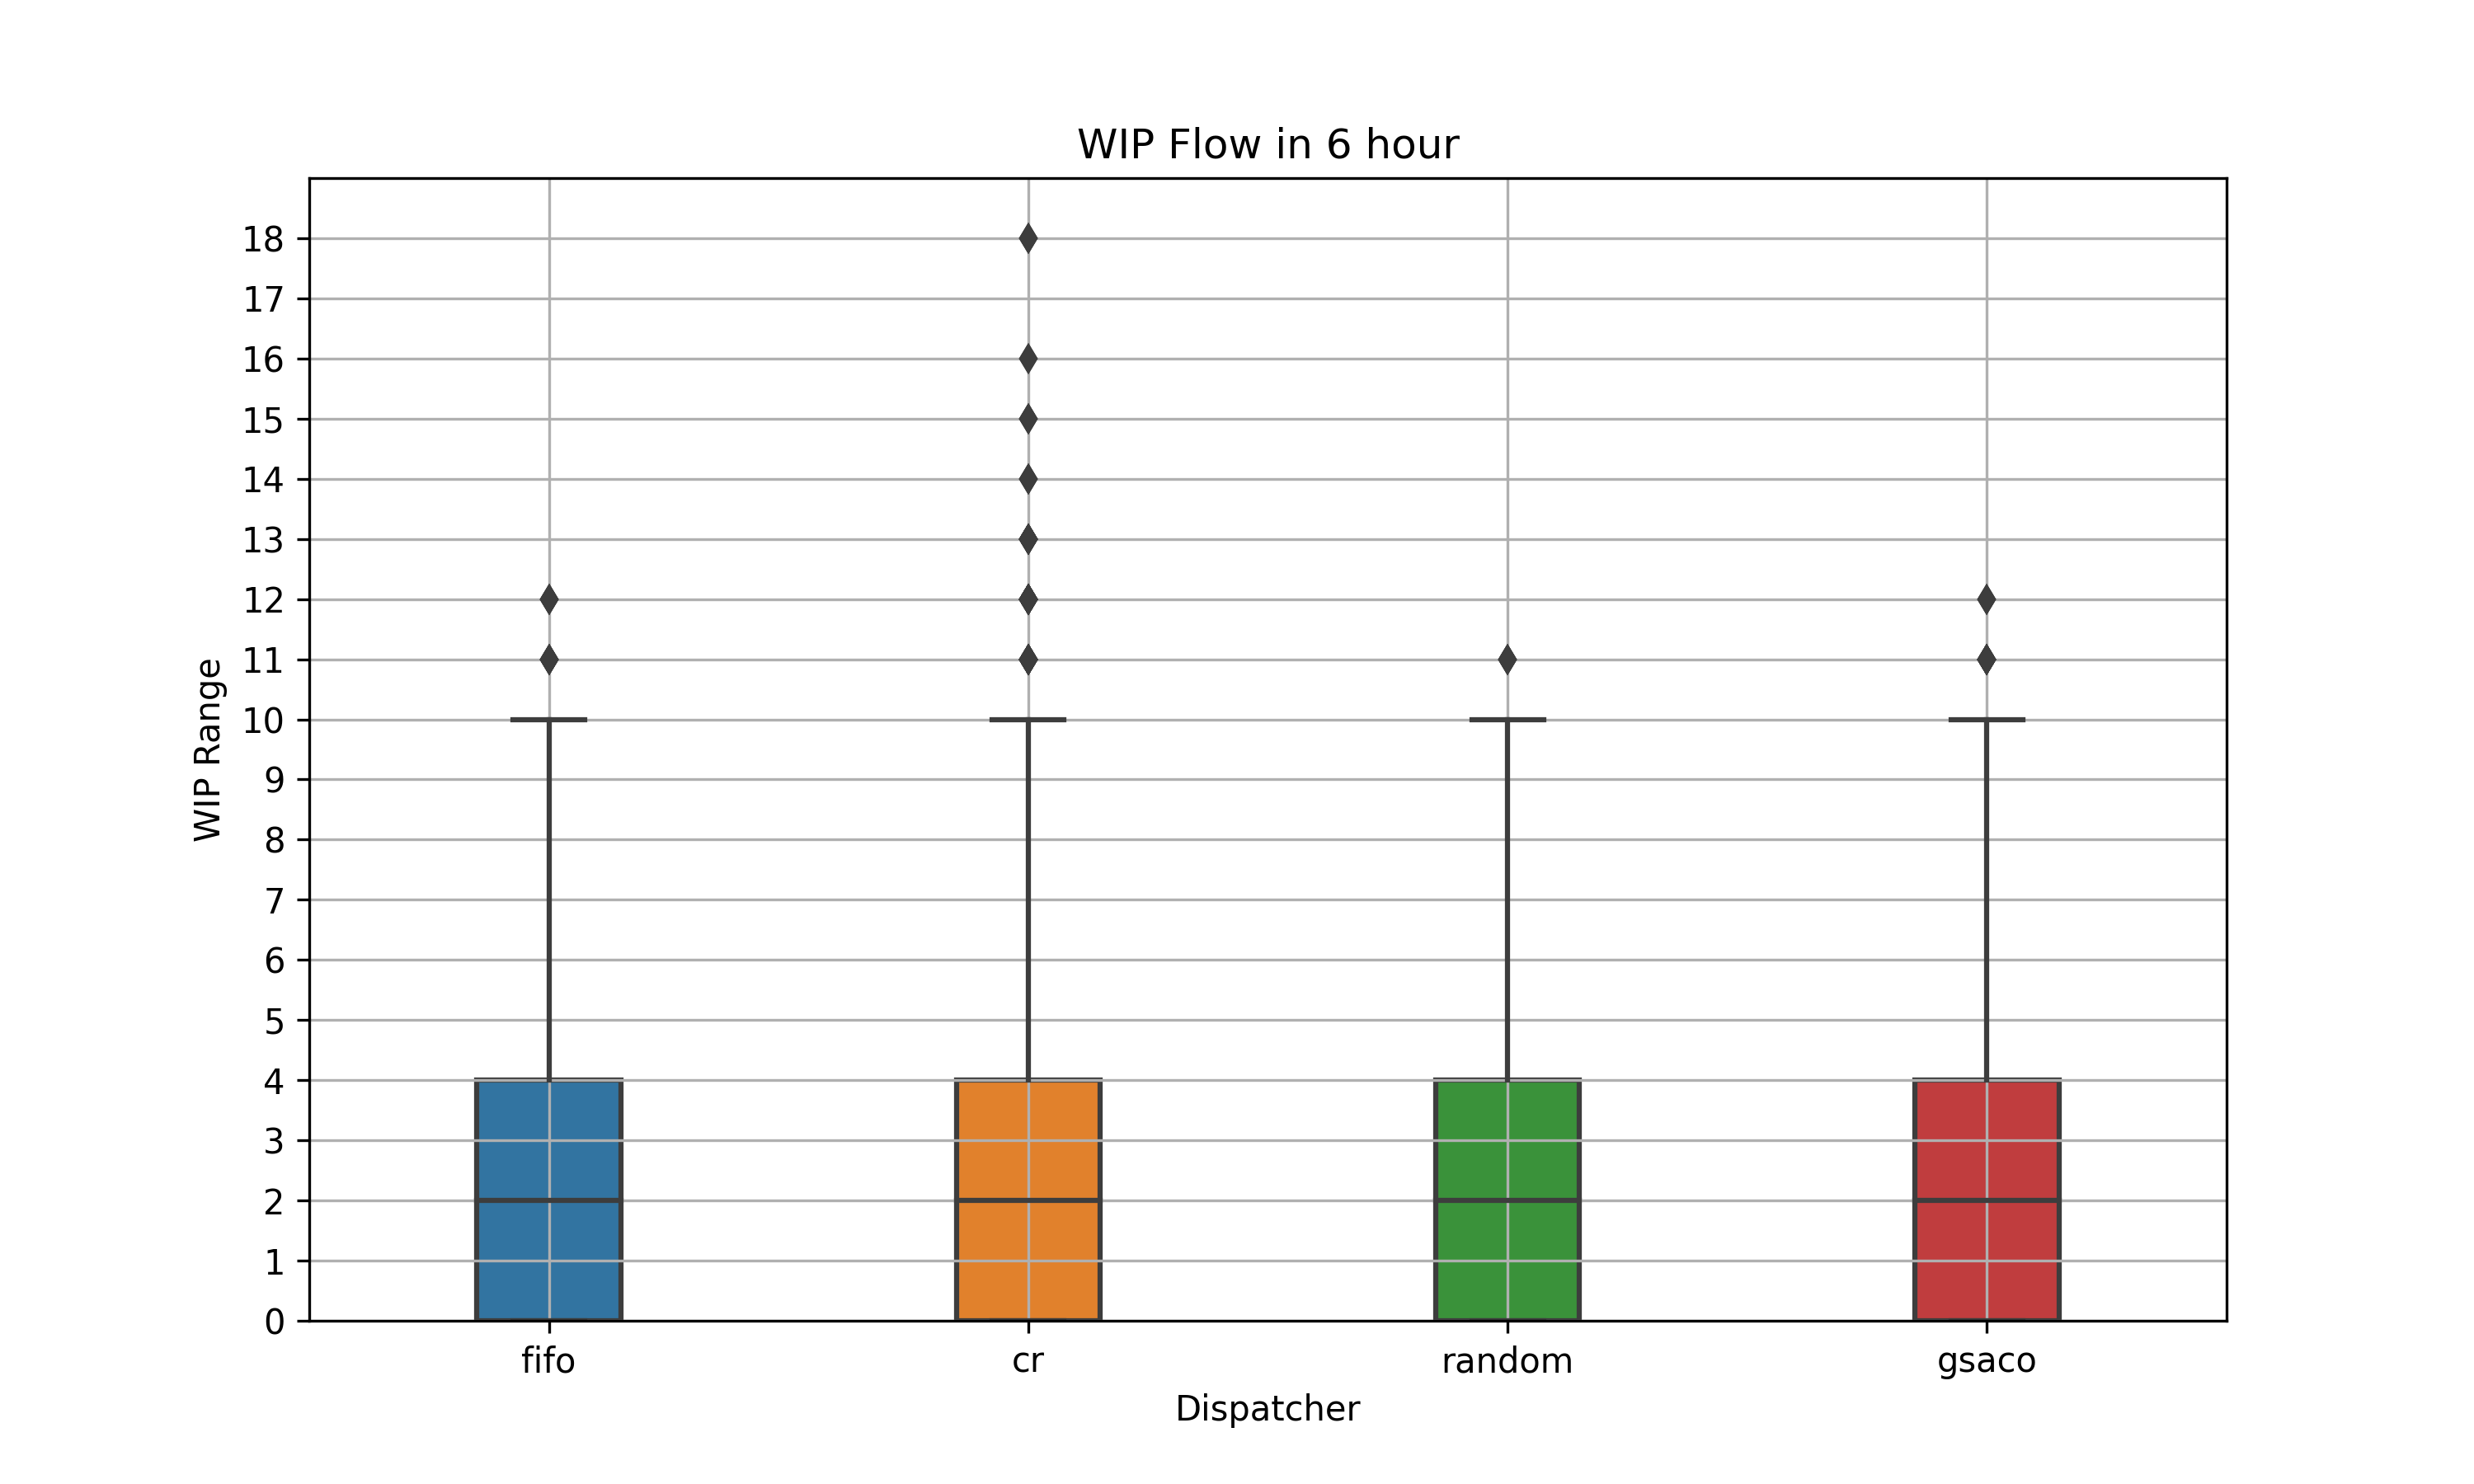
\includegraphics[width=\textwidth]{LVHM/period_21600s.png}
		% \caption{}
		% \label{fig:pp6}
	\end{subfigure}
    \caption{WIP flow for LV/HM}
    \label{fig:wip-flows-LVHM}
\end{figure}


\begin{figure}[ht]
	\centering
	\begin{subfigure}{0.32\textwidth}
		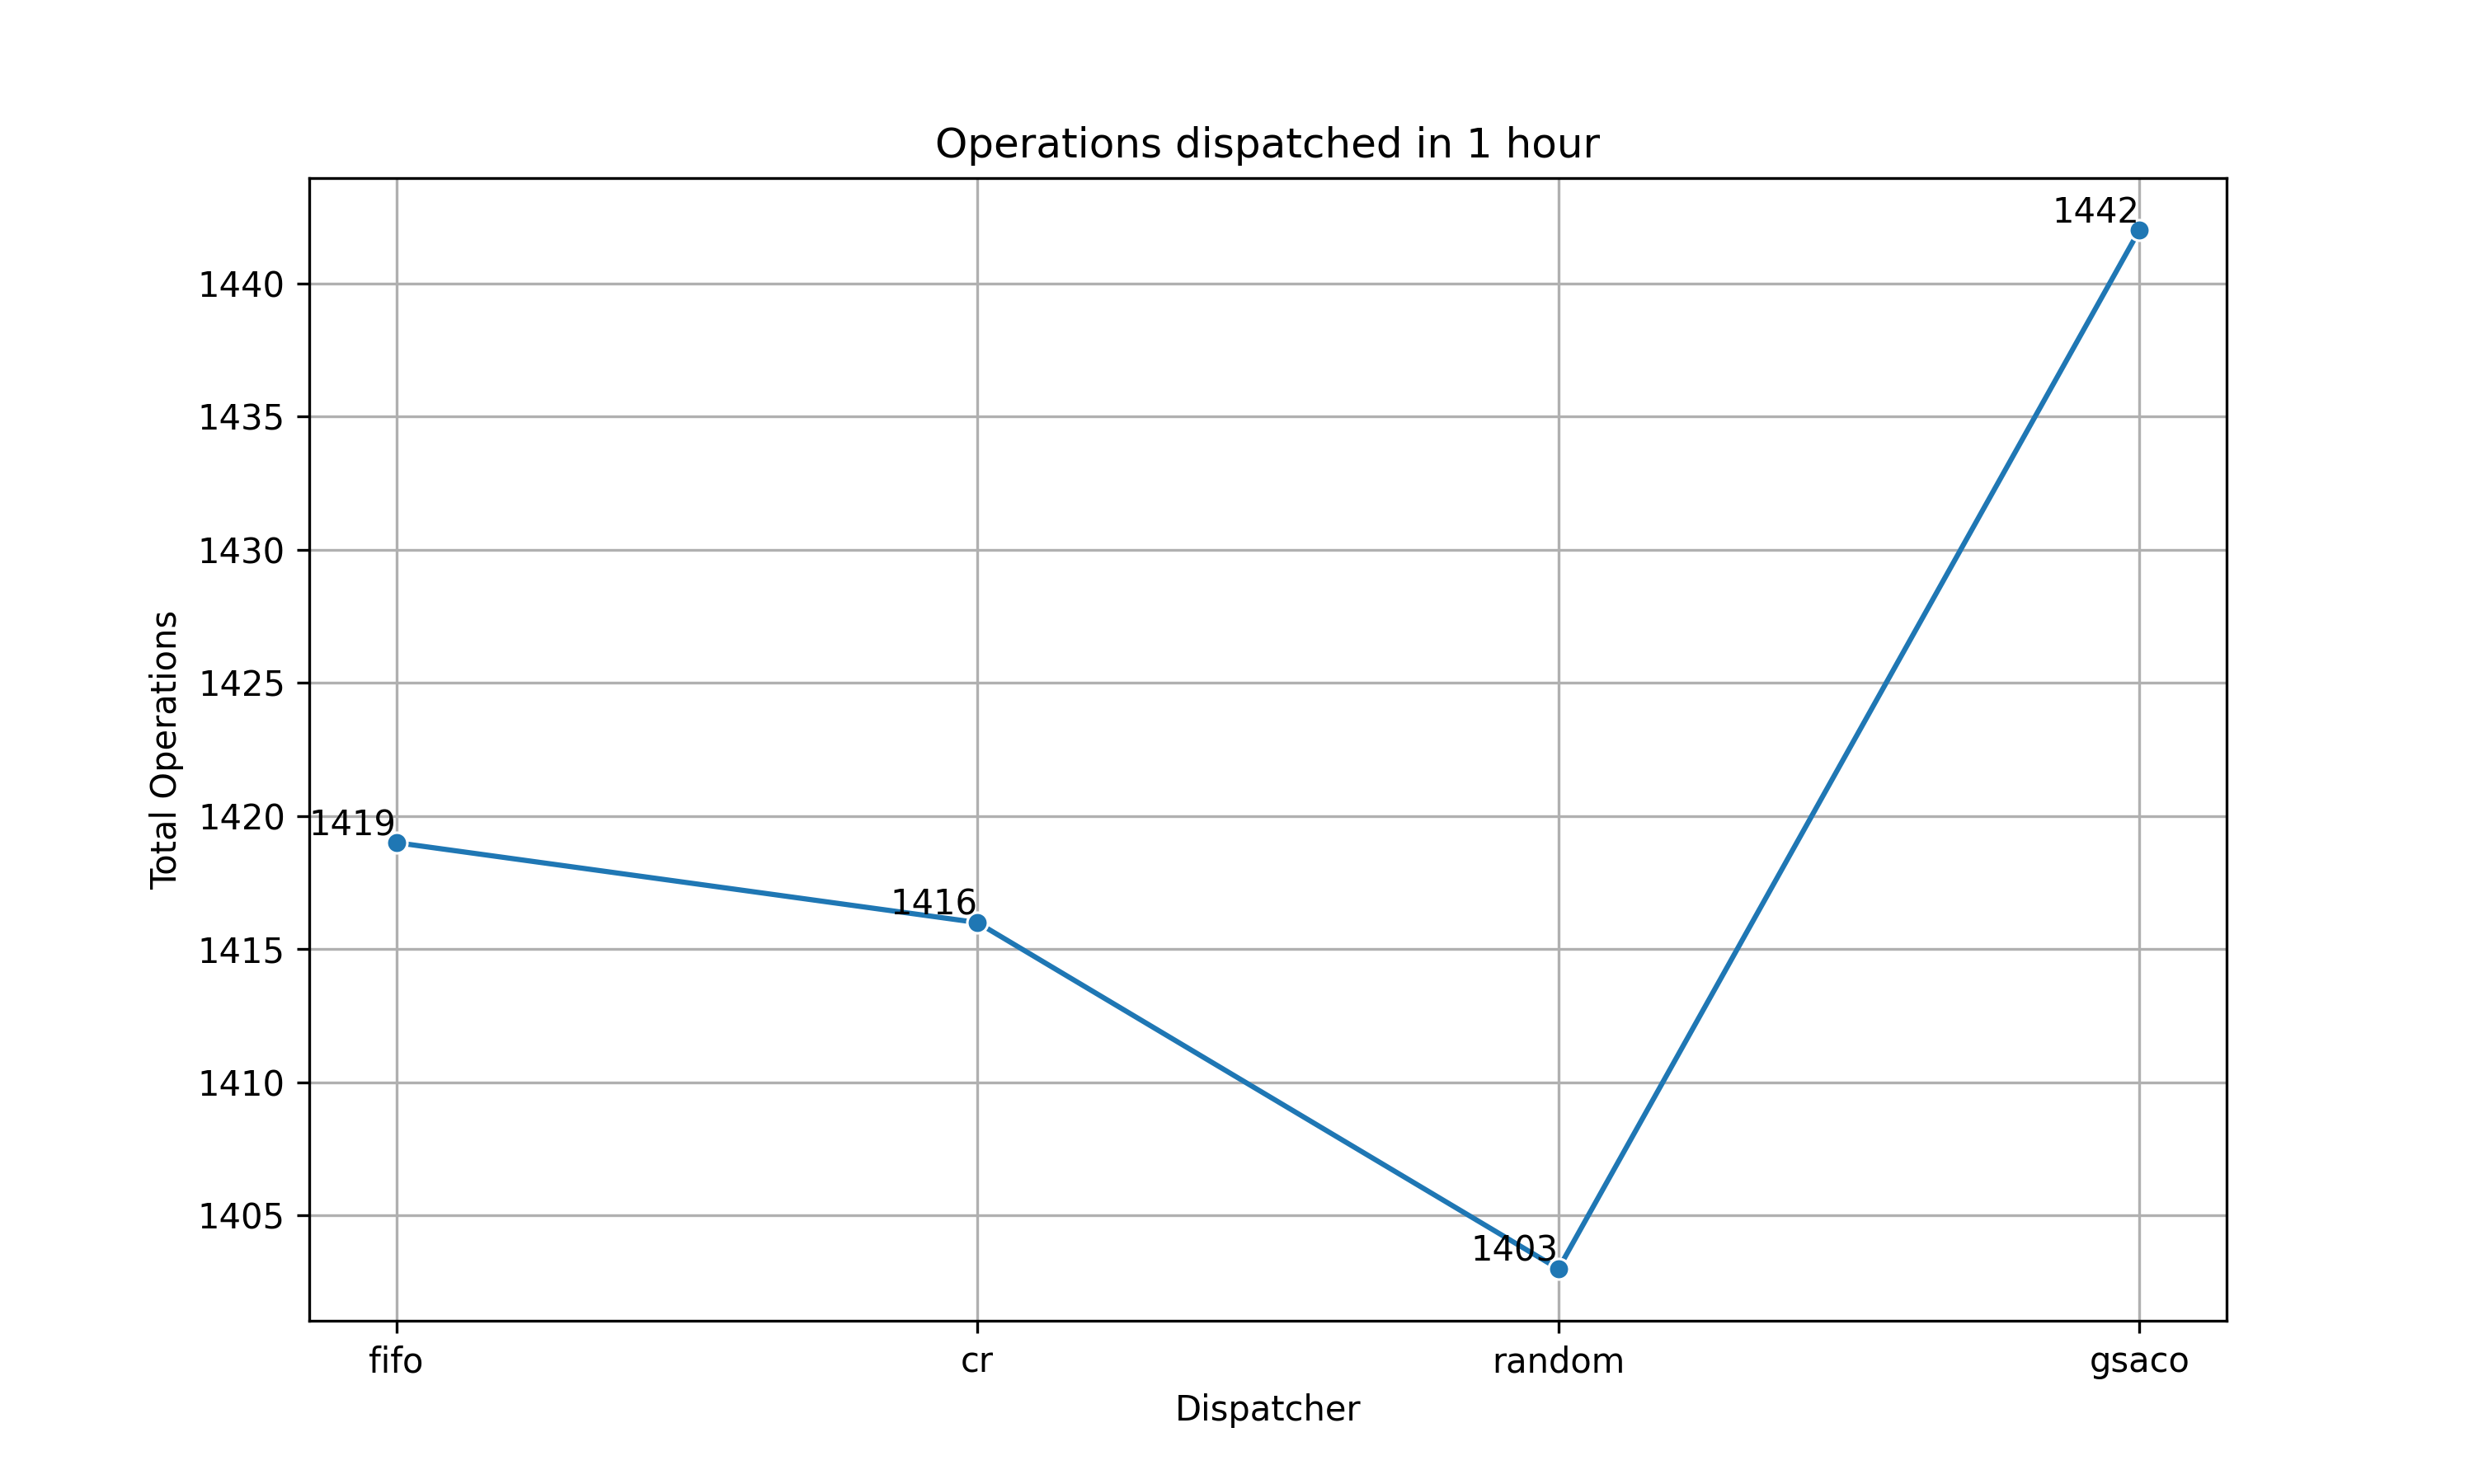
\includegraphics[width=\textwidth]{LVHM/total_operations_3600s.png}
		% \caption{}
		% \label{fig:oo1}
	\end{subfigure}\hfill
	\begin{subfigure}{0.32\textwidth}
		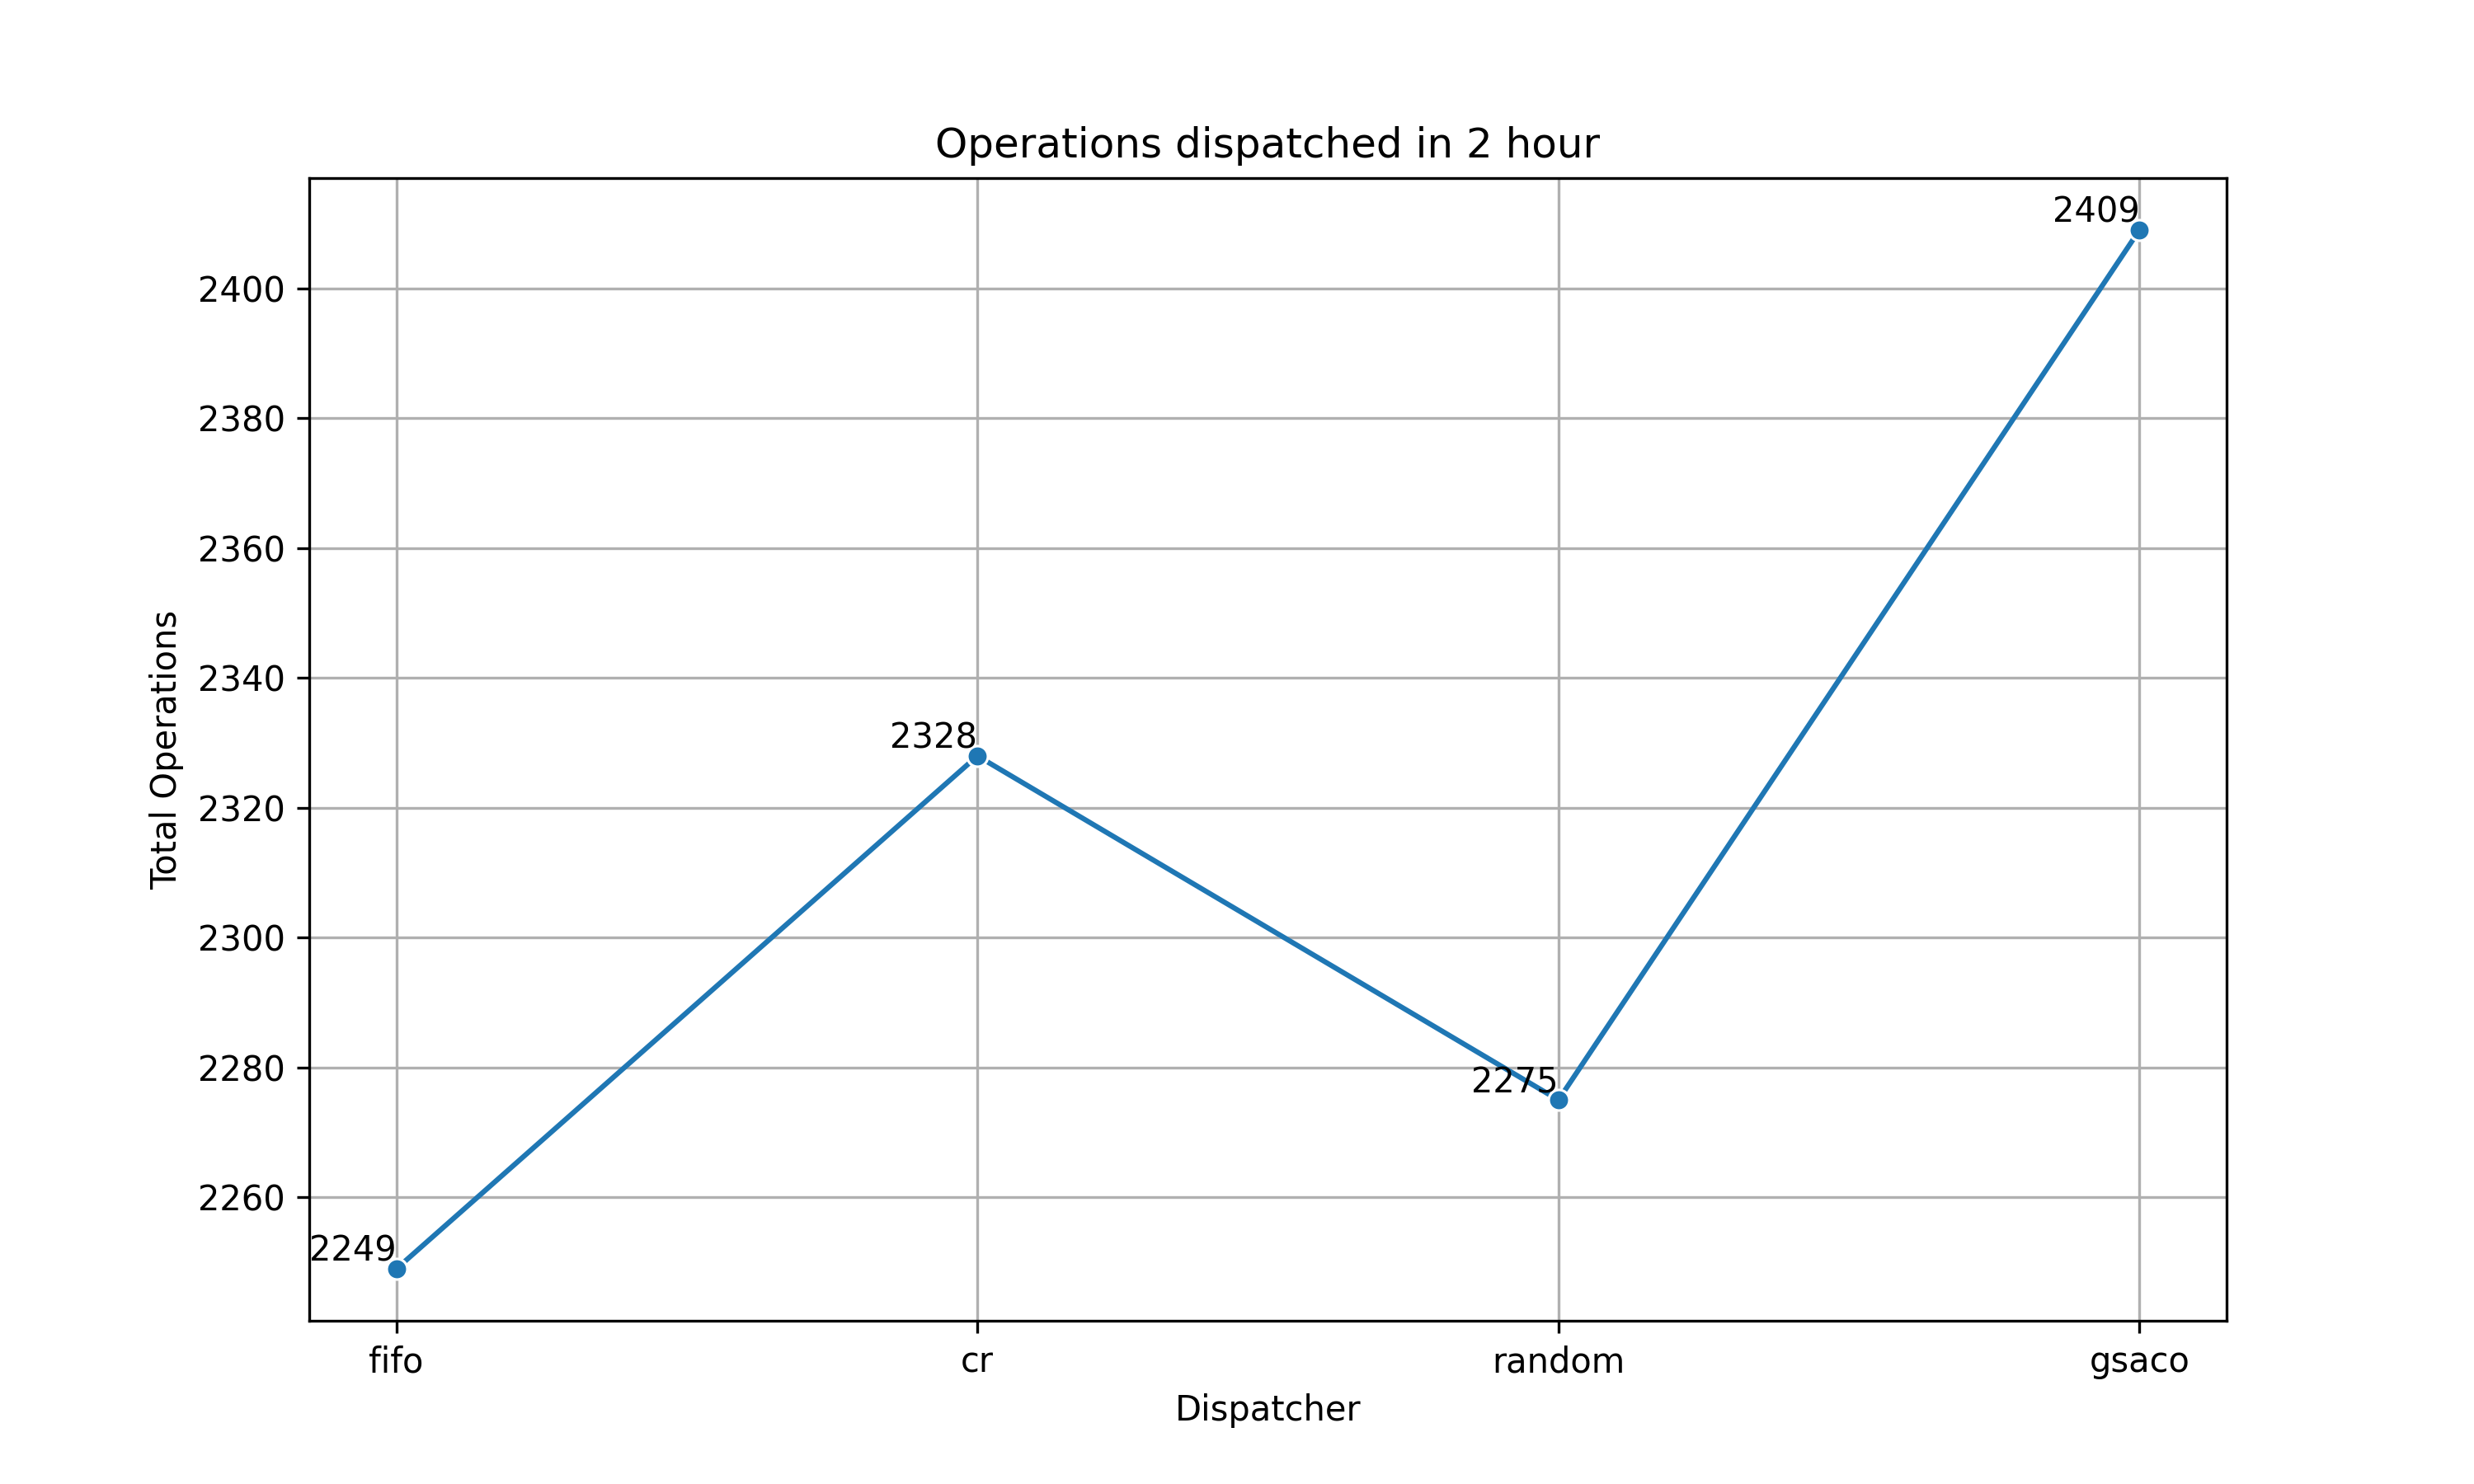
\includegraphics[width=\textwidth]{LVHM/total_operations_7200s.png}
		% \caption{}
		% \label{fig:oo2}
	\end{subfigure}\hfill
	\begin{subfigure}{0.32\textwidth}
		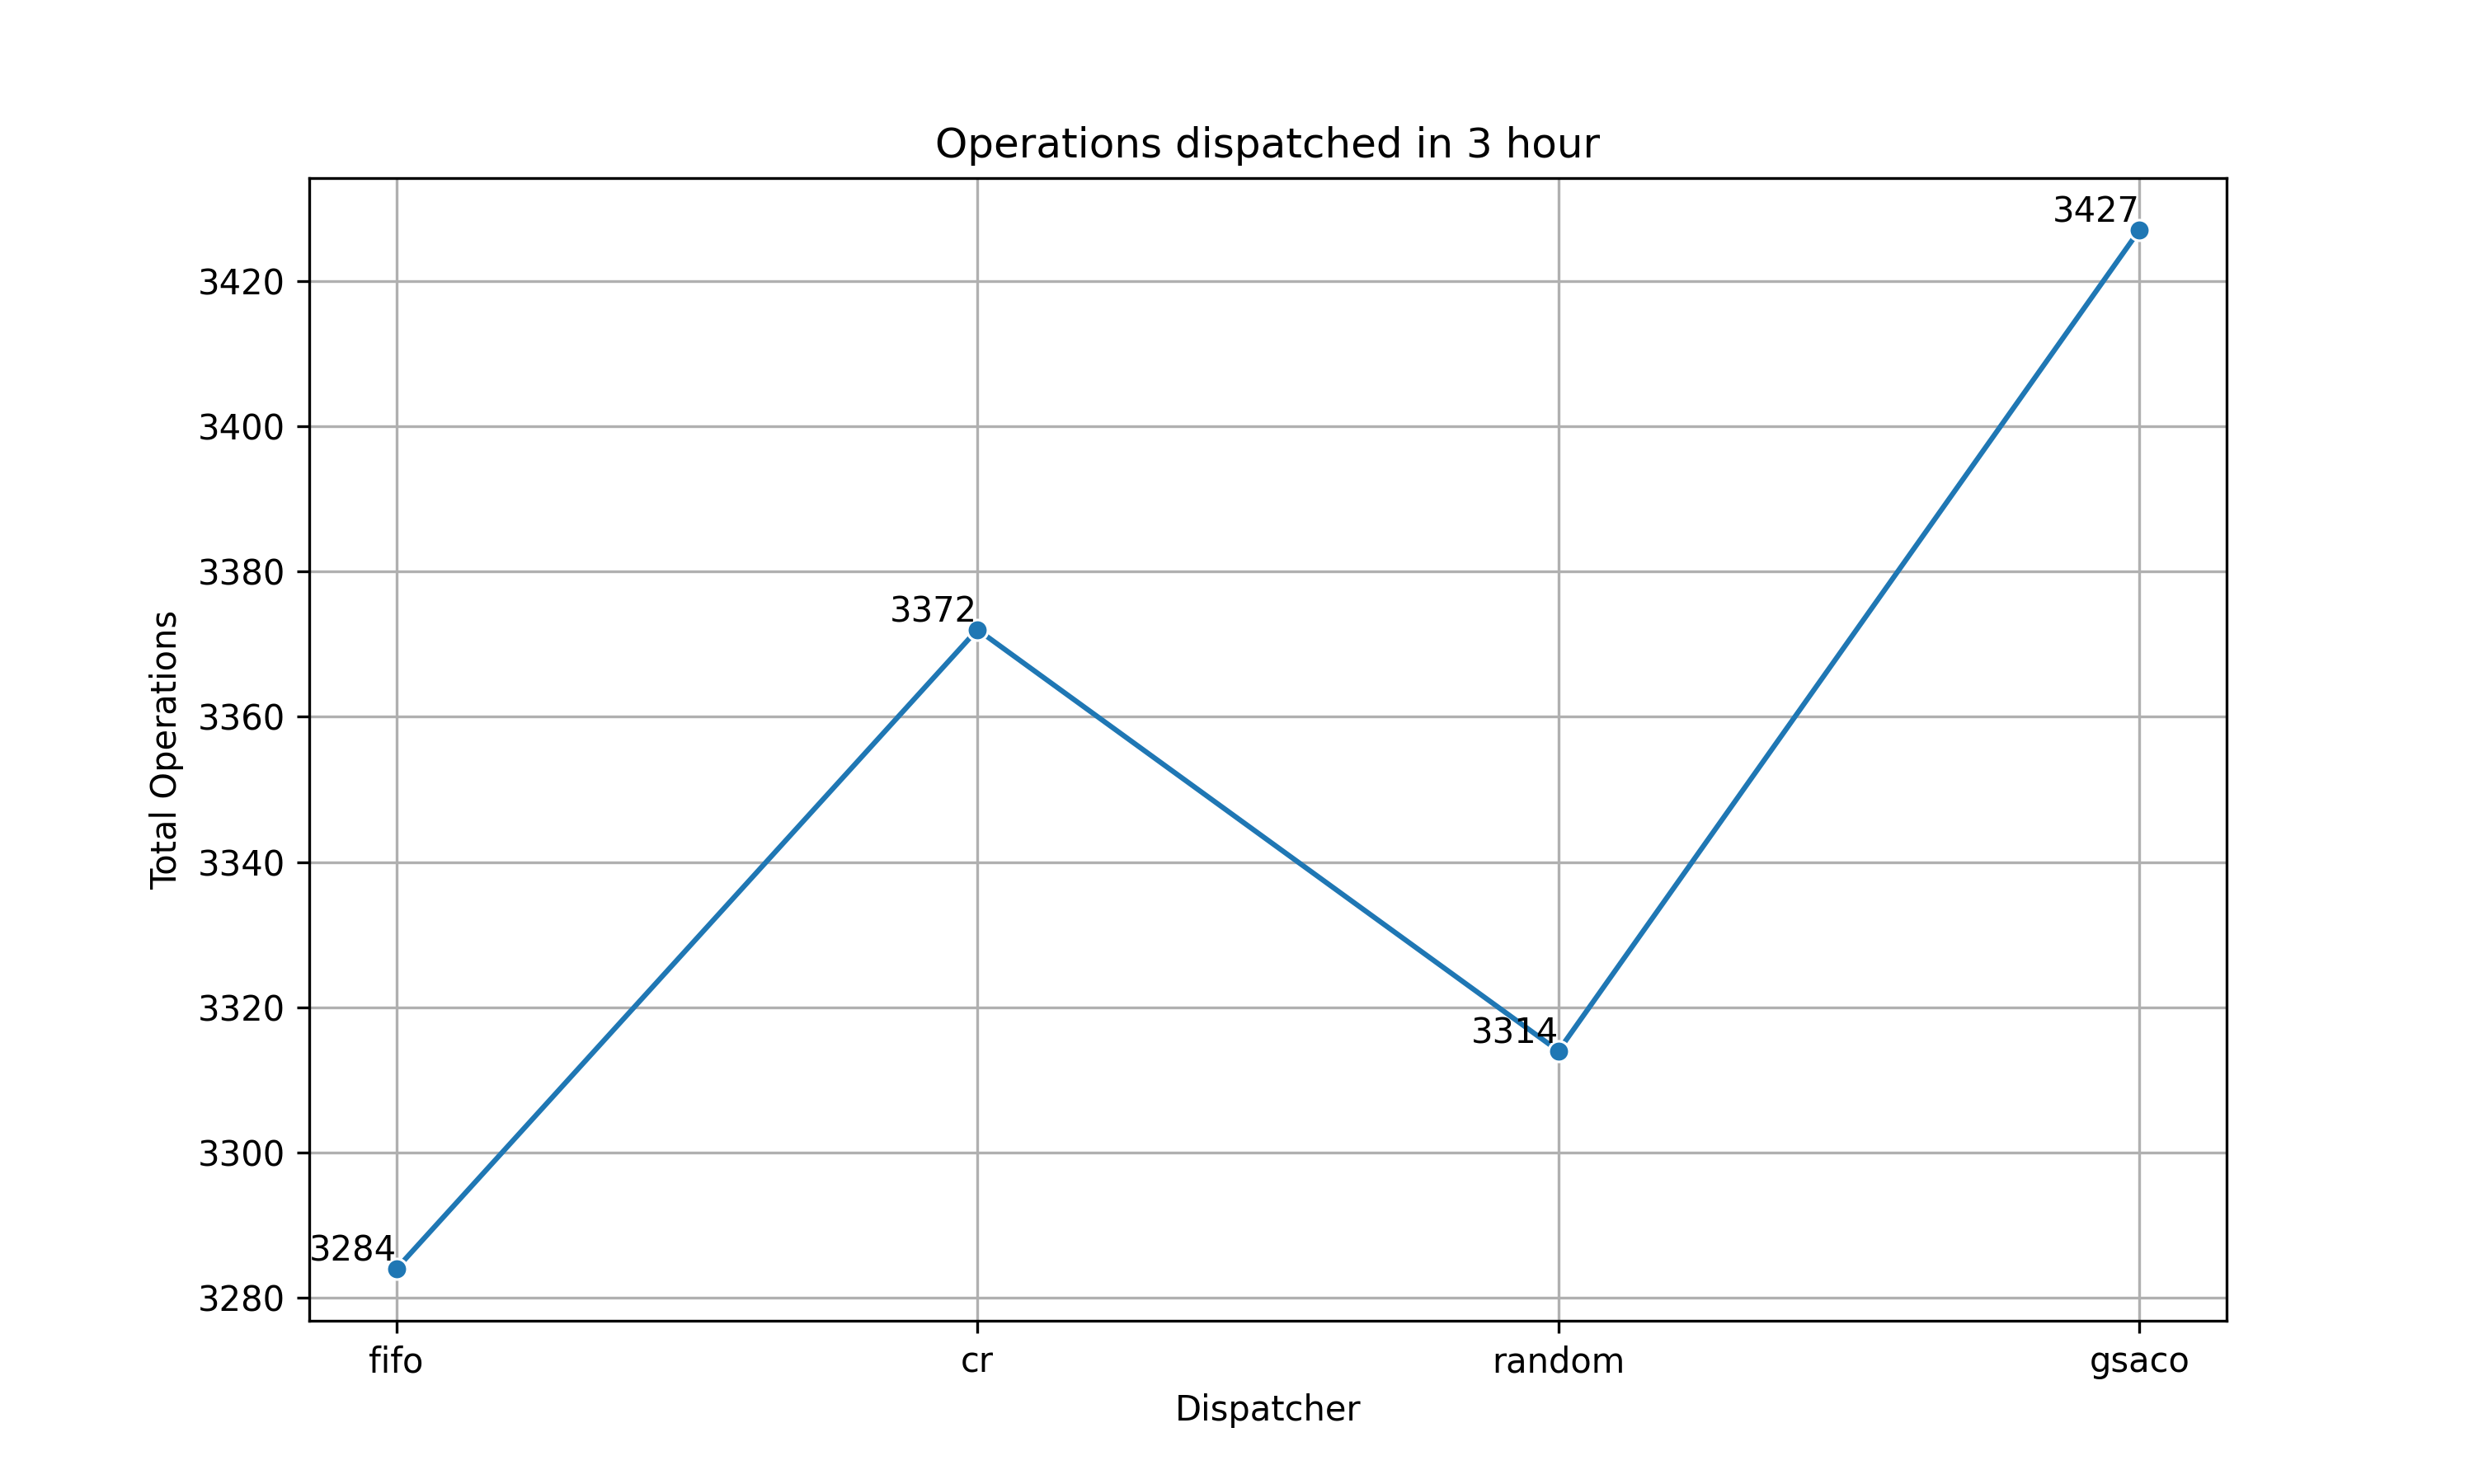
\includegraphics[width=\textwidth]{LVHM/total_operations_10800s.png}
		% \caption{}
		% \label{fig:oo3}
	\end{subfigure}
	\begin{subfigure}{0.32\textwidth}
		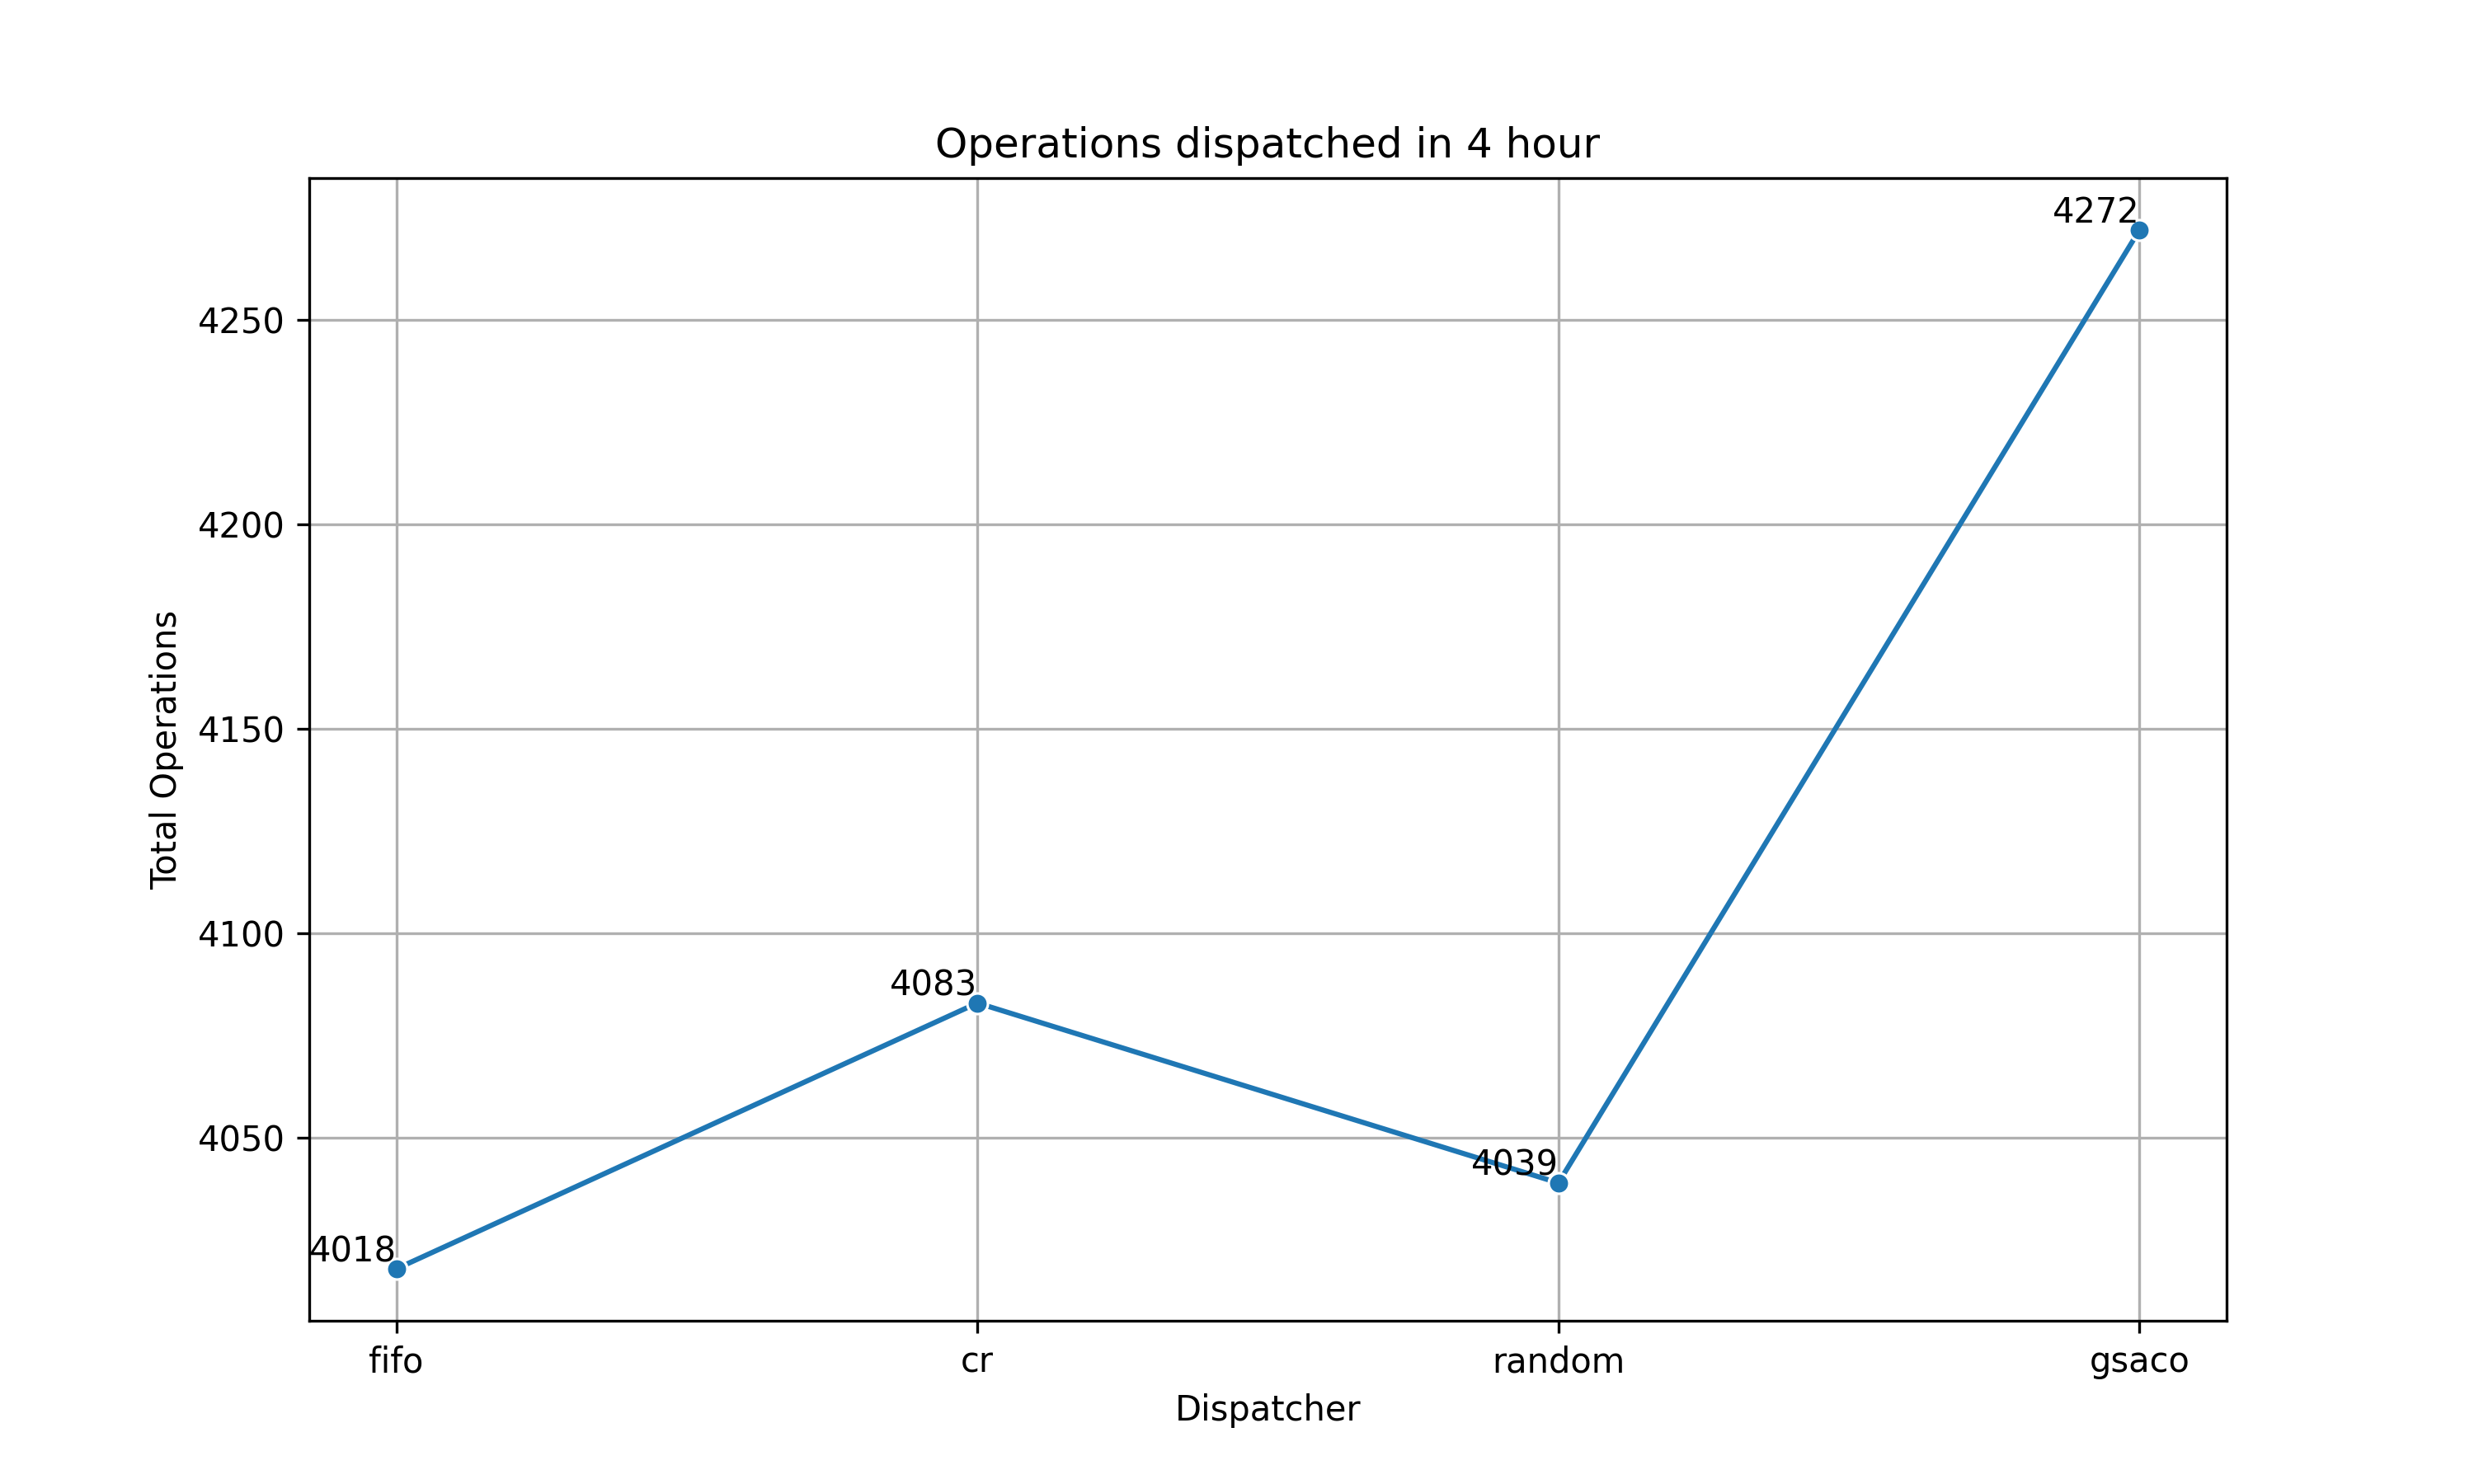
\includegraphics[width=\textwidth]{LVHM/total_operations_14400s.png}
		% \caption{}
		% \label{fig:oo4}
	\end{subfigure}\hfill
	\begin{subfigure}{0.32\textwidth}
		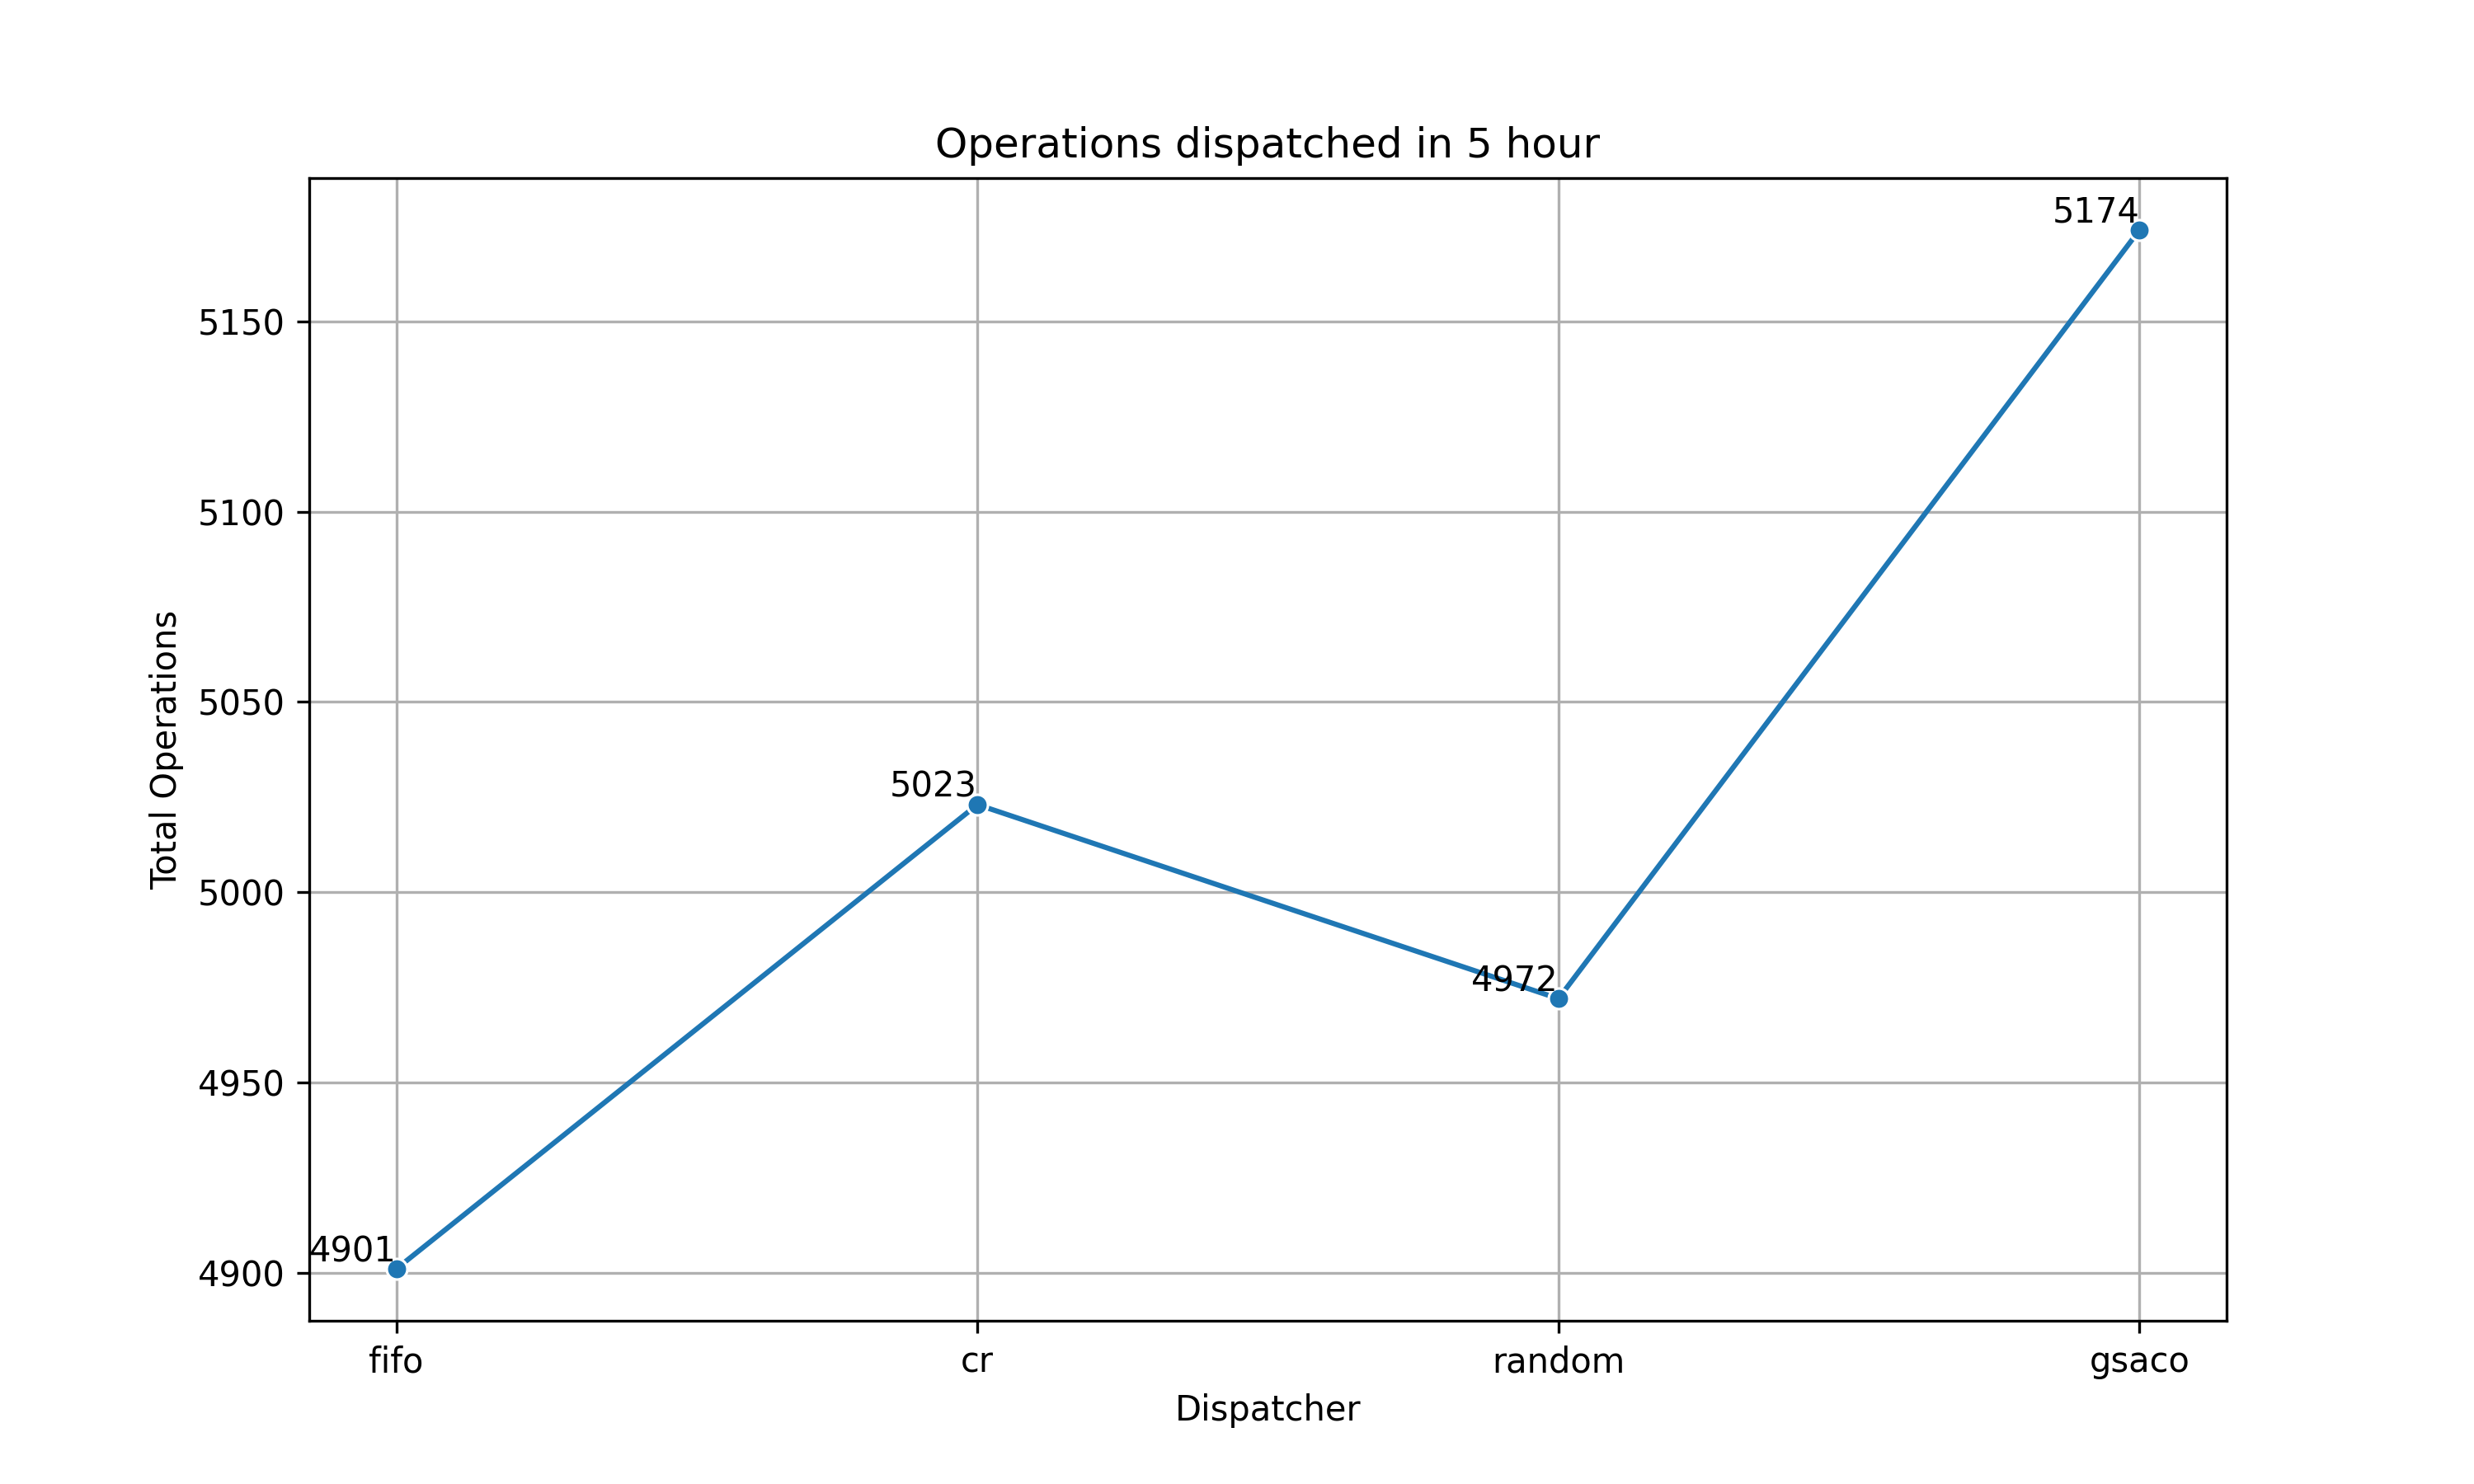
\includegraphics[width=\textwidth]{LVHM/total_operations_18000s.png}
		% \caption{}
		% \label{fig:oo5}
	\end{subfigure}\hfill
	\begin{subfigure}{0.32\textwidth}
		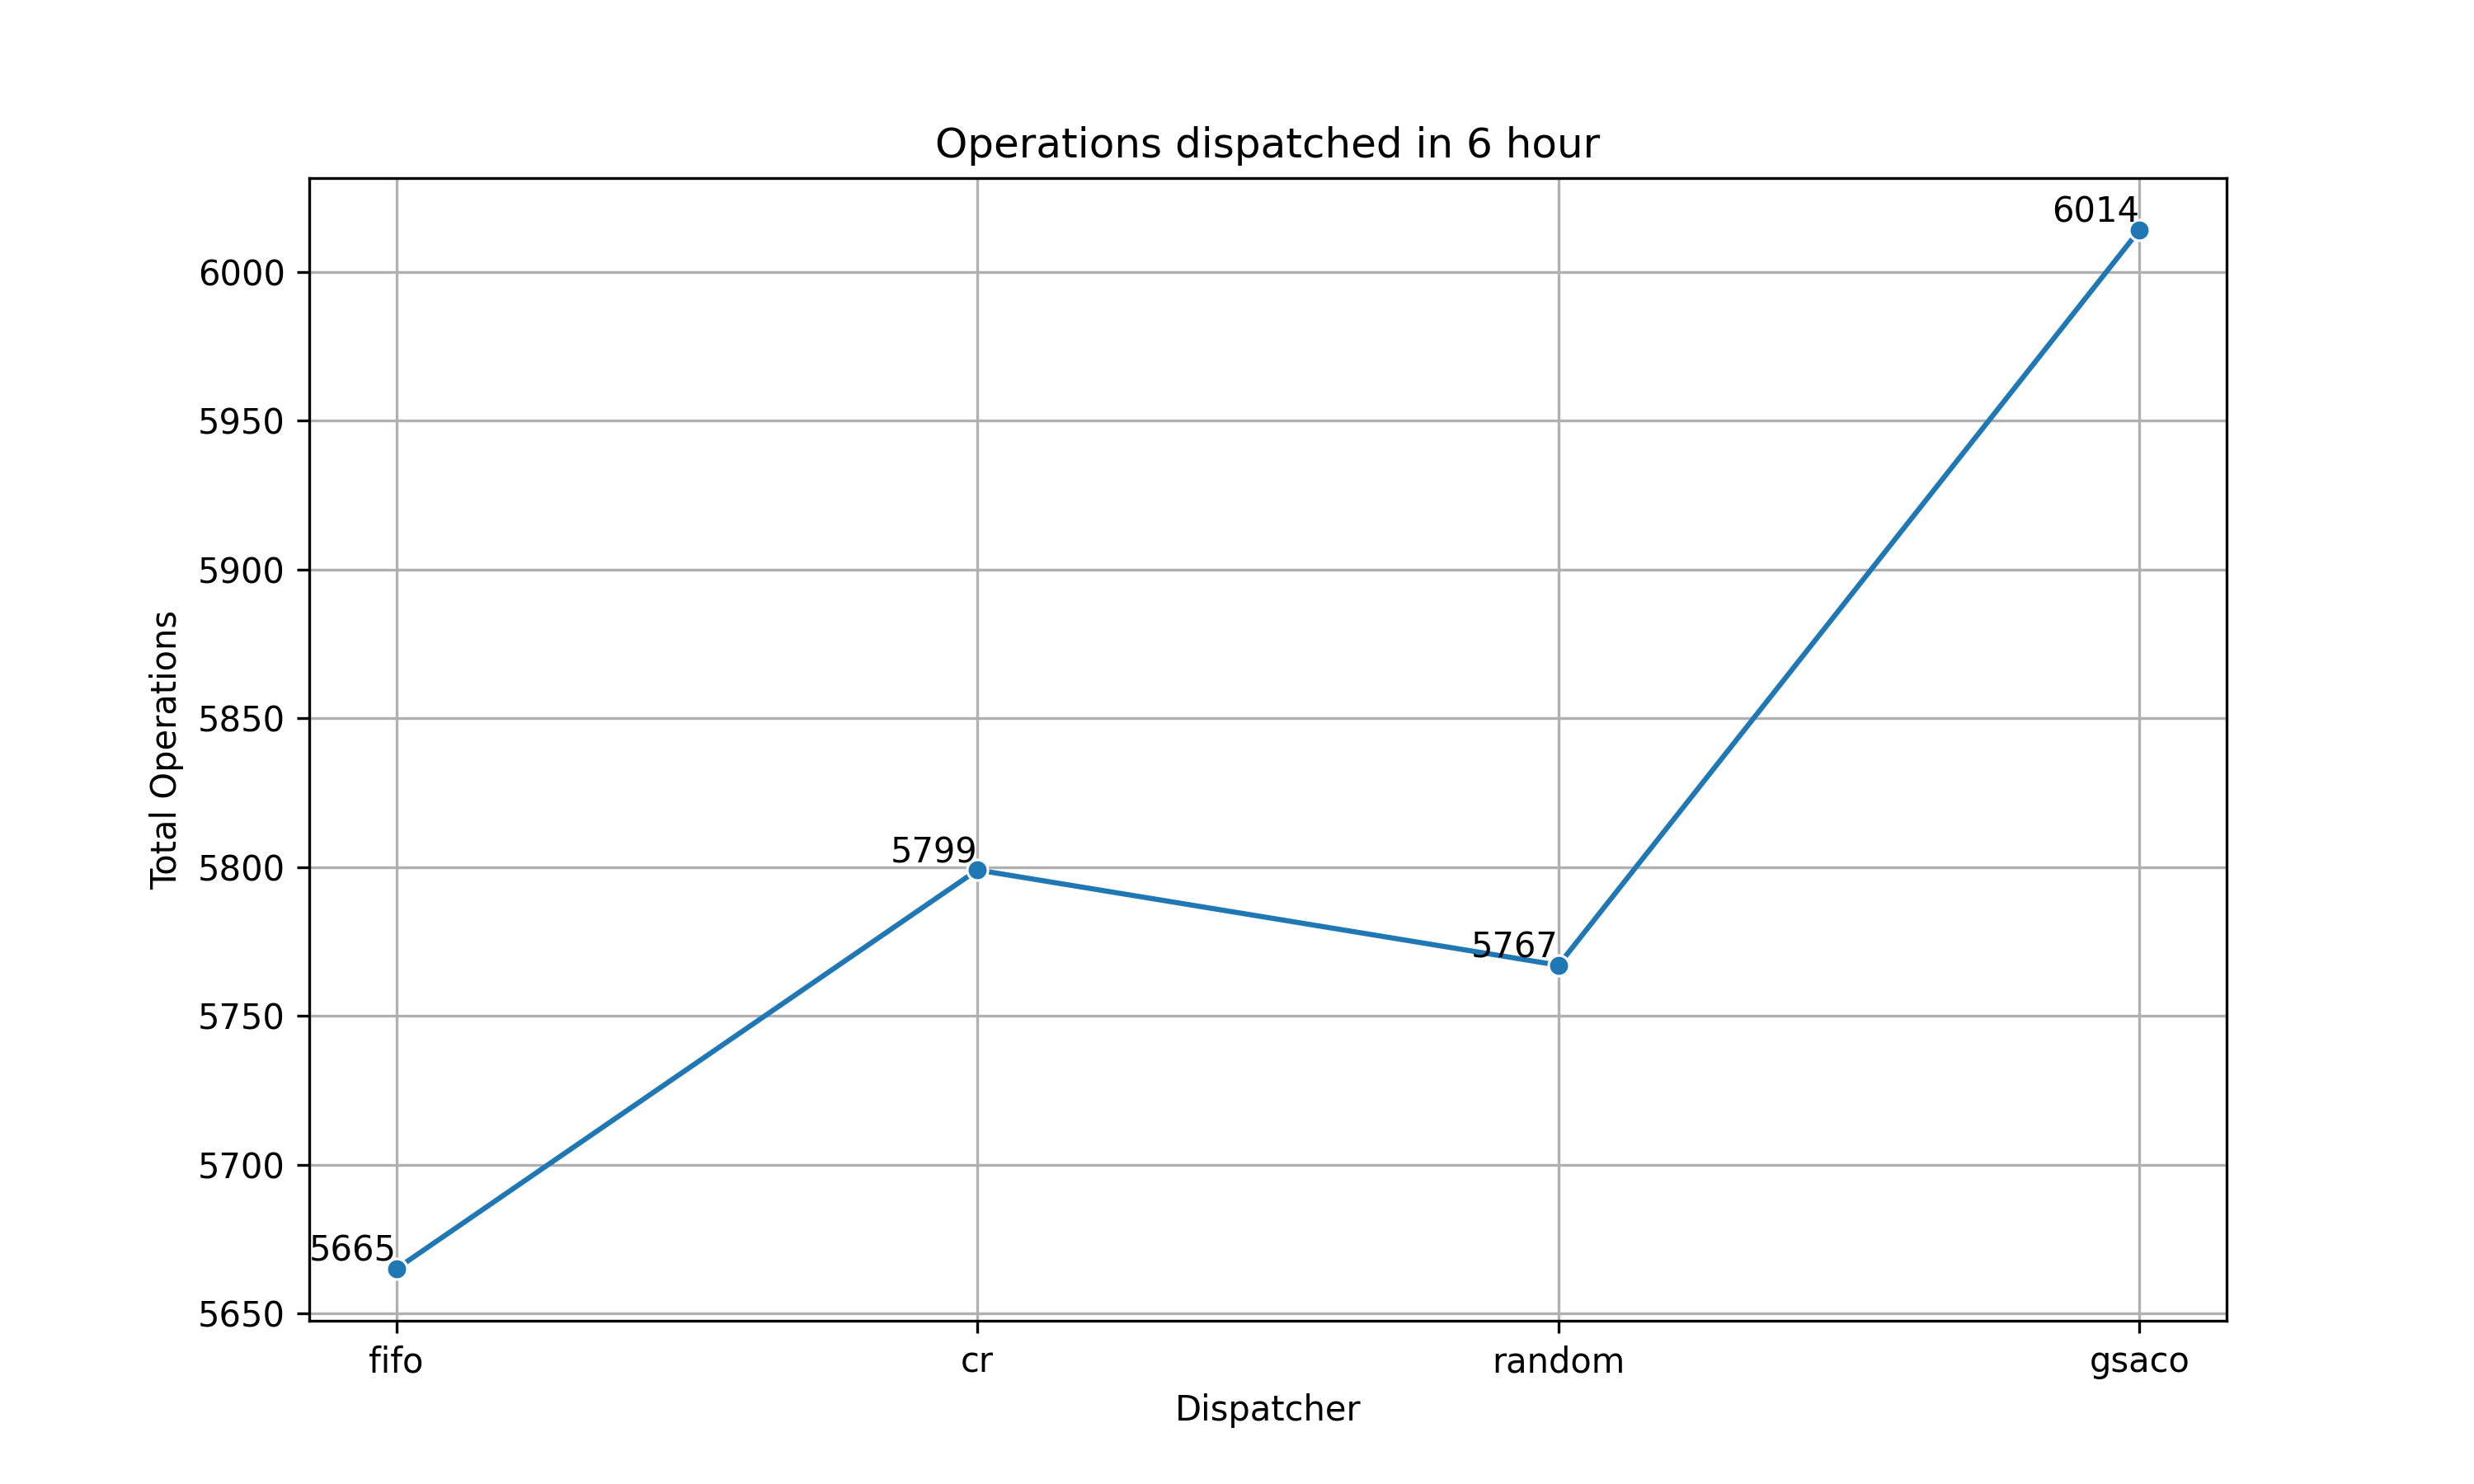
\includegraphics[width=\textwidth]{LVHM/total_operations_21600s.png}
		% \caption{}
		% \label{fig:oo6}
	\end{subfigure}
	\caption{Total operations completed LV/HM}
	\label{fig:totalopsLVHM}
\end{figure}